\documentclass[9pt]{article}

\usepackage[utf8]{inputenc}
\usepackage{geometry}
\geometry{
    a4paper,
    total={170mm,257mm},
    left=15mm,
    right=15mm,
    top=20mm,
    bottom=20mm,
}
\usepackage{multicol}
\usepackage[font=small,labelfont=bf]{caption}
\setlength{\columnsep}{0.25cm}
\usepackage[inline]{enumitem}
\usepackage{amssymb}
\usepackage{xcolor}
\usepackage{mathtools} 
\setlength{\parindent}{0em}
\setlength{\parsep}{0em}
\usepackage{tikz}
\setlength{\parskip}{0em}
\usetikzlibrary{decorations.pathmorphing,patterns}
\usepackage[american,cuteinductors]{circuitikz}
\usetikzlibrary{shapes,arrows,circuits,calc,babel}
% Definition of blocks:
\tikzset{%
  block/.style    = {draw, thick, rectangle, minimum height = 3em,
    minimum width = 3em},
  sum/.style      = {draw, circle, node distance = 2cm}, % Adder
  input/.style    = {coordinate}, % Input
  output/.style   = {coordinate} % Output
}
% Defining string as labels of certain blocks.
\newcommand{\suma}{\Large$+$}
\newcommand{\inte}{$\displaystyle \int$}
\newcommand{\derv}{\huge$\frac{d}{dt}$}

\def\mf{\ensuremath\mathbf}
\def\mb{\ensuremath\mathbb}
\def\mc{\ensuremath\mathcal}
\def\lp{\ensuremath\left(}
\def\rp{\ensuremath\right)}
\def\lv{\ensuremath\left\lvert}
\def\rv{\ensuremath\right\rvert}
\def\lV{\ensuremath\left\lVert}
\def\rV{\ensuremath\right\rVert}
\def\lc{\ensuremath\left\{}
\def\rc{\ensuremath\right\}}
\def\ls{\ensuremath\left[}
\def\rs{\ensuremath\right]}
\def\bmx{\ensuremath\begin{bmatrix*}[r]}
\def\emx{\ensuremath\end{bmatrix*}}
\def\bmxc{\ensuremath\begin{bmatrix*}[c]}
\def\emxc{\ensuremath\end{bmatrix*}}
% \def\t{\lp t\rp}
% \def\k{\ls k\rs}

\newcommand{\demoex}[2]{\onslide<#1->\begin{color}{black!60} #2 \end{color}}
\newcommand{\demoexc}[3]{\onslide<#1->\begin{color}{#2} #3 \end{color}}
\newcommand{\anim}[3]{\onslide<#1->{\begin{color}{#2!60} #3 \end{color}}}
\newcommand{\ct}[1]{\lp #1\rp}
\newcommand{\dt}[1]{\ls #1\rs}

\renewcommand{\familydefault}{\sfdefault}

\begin{document}
\begin{center}
\begin{Large}
\textbf{Linear Systems: Assignment}
\end{Large}
\end{center}
\vspace{0.2cm}

\begin{multicols}{2}

% -*- root: ../assignment.tex -*-

\subsection*{Vectors}
\begin{enumerate}
    \item Is this set of vectors $\left\{\begin{bmatrix}2 \\ 1 \\ 1\end{bmatrix}, \begin{bmatrix}0 \\ 0\\ 0\end{bmatrix}, \begin{bmatrix}0 \\ 1 \\ 0\end{bmatrix}\right\}$ independent? Explain your answer.

    \item Consider a set of finite duration discrete-time real signals $X_N = \lc x\dt{n} \big\vert x\dt{n} \in \mb{R}, \,\forall 0 \leq n \leq N-1\rc$. Does this set form a vector space? Explain your answer. Would $X_N$ still be a vector spaces if the signals were binary signals? i.e. $x\dt{n} \in \mb{B}$, where $\mb{B} = \lc 0, 1\rc$ with the binary addition and multiplication operations defined as the following,

    \begin{minipage}[h]{.45\textwidth}
        \centering
        \begin{tabular}{|c|c|c|c|}
        \hline
        $a$ & $b$ & $a+b$ & $a \times b$ \\ \hline
        0 & 0 & 0   & 0     \\ \hline
        0 & 1 & 1   & 0     \\ \hline
        1 & 0 & 1   & 0     \\ \hline
        1 & 1 & 0   & 1     \\ \hline
        \end{tabular}\\
        \captionof{table}{\small{Addition and Multiplication operation for binary numbers.}}
    \end{minipage}

    \item Prove the following for $\mathbf{x}, \mathbf{y} \in \mathbb{R}^n$
    \begin{enumerate}
        \item {\small \textbf{Triangle Inequality}}:
        $$\left\lVert \mathbf{x} + \mathbf{y}\right\rVert \leq \left\lVert \mathbf{x}\right\rVert + \left\lVert \mathbf{y}\right\rVert$$
        \item {\small \textbf{Backward Triangle Inequality}}:
        $$\left\lVert \mathbf{x} - \mathbf{y}\right\rVert  \geq \left\lvert \left\lVert \mathbf{x}\right\rVert - \left\lVert \mathbf{y}\right\rVert \right\rvert$$
        \item {\small \textbf{Parallelogram Identity}}:
        $$\frac{1}{2} \left(\left\lVert \mathbf{x} + \mathbf{y}\right\rVert^2 + \left\lVert \mathbf{x} - \mathbf{y}\right\rVert^2 \right) = \left\lVert \mathbf{x}\right\rVert^2 + \left\lVert \mathbf{y}\right\rVert^2$$
    \end{enumerate}

    \item Consider a set of vectors $\mathbf{x}, \mathbf{y} \in \mathbb{R}^n$. When is $\left\lVert \mathbf{x} - \mathbf{y} \right\rVert = \left\lVert \mathbf{x} + \mathbf{y}\right\rVert$? What can you say about the geometry of the vectors $\mathbf{x},\,\mathbf{y},\,\mathbf{x} - \mathbf{y}$ and $\mathbf{x} + \mathbf{y}$?
    
    \item If $S_1, S_2 \subseteq V$ are subspaces of $V$, the is $S_1 \cap S_2$ a subspace? Demonstrate your answer.

    \item Consider two sets of vectors $V = \lc \mf{v}_1, \mf{v}_2, \ldots \mf{v}_n\rc$ and $W = \lc \mf{w}_1, \mf{w}_2, \ldots, \mf{w}_n, \mf{u}\rc$. Prove that if $span\ct{V} = span\ct{W}$, then $\mf{u} \in span\ct{V}$.
    
    \item Prove that the sum of two subspaces $S_1, S_2 \subseteq V$ is a subspace.
    
    \item Consider a vector $\mathbf{v} = \begin{bmatrix*}v_1\\v_2\\\vdots\\v_n\end{bmatrix*}$. Express the following in-terms of inner product between a vector $\mathbf{u}$ and $\mathbf{v}$, and in each case specify the vector $\mathbf{u}$.
    \begin{enumerate}
        \item $\sum_{i=1}^nv_i$
        \item $\frac{1}{n}\sum_{i=1}^nv_i$
        \item $\sum_{i=1}^nv_ix^{\left(n - i\right)}$, where $x \in \mathbb{R}$
        \item $\frac{1}{n-1}\sum_{i=1}^n\left(v_i - \frac{1}{n}\sum_{i=1}^nv_i \right)^2$
        \item $\frac{1}{5}\sum_{i=3}^5 v_i$
        \item $\sum_{i=1}^{n-1} \left(v_{i+1} - v_i\right)$
        \item $\sqrt{v_n}$
        \item $\sum_{i=1}^nw_iv_i^2$
    \end{enumerate}
    
    \item Which of the following are linear functions of $\left\{x_1, x_2, \ldots,x_n\right\}$?
    \begin{enumerate}
        \item $\min_i \left\{x_i\right\}_{i=1}^{n}$
        \item $\left(\sum_{i=1}^n x_i^2\right)^{1/2}$
        \item $x_6$
    \end{enumerate}
    
    \item Consider a linear function $f: \mathbb{R}^n \rightarrow \mathbb{R}$. Prove that every linear function of this form can be represented in the following form.
    \[ y = f\left(\mathbf{x}\right) = \mathbf{w}^T\mathbf{x} = \sum_{i=1}^{n}w_ix_i, \,\,\,\,\, \mathbf{x}, \mathbf{w} \in \mathbb{R}^n \]

    \item An \textit{affine} function $f$ is defined as the sum of a linear function and a constant. It can in general be represented in the form, 
    \[ y = f\left(\mathbf{x}\right) = \mathbf{w}^T\mathbf{x} + \beta, \,\,\,\,\, \mathbf{x}, \mathbf{w} \in \mathbb{R}^n, \, \beta \in \mathbb{R} \]
    Prove that affine functions are not linear. Prove that any affine function can be represented in the form $\mathbf{w}^T\mathbf{x} + \beta$.

    \item Consider a function $f: \mathbb{R}^3 \rightarrow \mathbb{R}$, such that,
    \[ f\left(\begin{bmatrix*}[r]1\\0\\0\end{bmatrix*}\right) = 2; \,\,
    f\left(\begin{bmatrix*}[r]0\\1\\0\end{bmatrix*}\right) = -3; \,\,
    f\left(\begin{bmatrix*}[r]0\\0\\1\end{bmatrix*}\right) = 1; \,\,\]
    Can you determine the following values of $f\left(\mathbf{x}\right)$, if you are told that $f$ is linear?
    \[ f\left(\begin{bmatrix*}[r]2\\2\\-2\end{bmatrix*}\right) = ?; \,\,\,
     f\left(\begin{bmatrix*}[r]-1\\2\\0\end{bmatrix*}\right) = ?; \,\,\,
     f\left(\begin{bmatrix*}[r]0.5\\0.6\\-0.1\end{bmatrix*}\right) = ?; \,\,\,\]
     Can you find out these values if you are told that $f$ is affine?
    
    \item For the previous question, (a) assume that $f$ is linear and find out $w \in \mathbb{R}^3$, such that $f\left(\mathbf{x}\right) = \mathbf{w}^T\mathbf{x}$; and (b) assume $f$ is affine and find out $\mathbf{w}, \beta$ such that $f\left(\right) = \mathbf{w}^T\mathbf{x} + \beta$.

    \item Consider the weighted norm of vector $\mathbf{v}$, defined as,
    \[ \left\lVert \mathbf{v}\right\rVert_{\mathbf{w}}^2 = \sum_{i=1}^{n}w_iv_i^2; \,\,\,\,\, \mathbf{w}=\begin{bmatrix*}w_1\\w_2\\\vdots\\w_n\end{bmatrix*} \]
    Is this a valid norm?\\

    \item Prove that the following modified version of the Cauchy-Bunyakovski-Schwartx Inequality is true.
    \[ \left\lvert \sum_{i=1}^{n} u_iv_iw_i \right\rvert \leq \left\lVert \mathbf{u}\right\rVert_\mathbf{w} \left\lVert \mathbf{v}\right\rVert_\mathbf{w} \]

    \item Consider a basis $B = \left\{\mathbf{b}_i\right\}_{i=1}^{n}$ of $R^n$. Let the vector $\mathbf{x}$ with the following representations in the standard and $B$ basis.
    \[ \mathbf{x} = \begin{bmatrix*}x_1\\x_2\\\vdots\\x_n\end{bmatrix*} = \sum_{i=1}^{n}x_i\mathbf{e}_i \,\,\,\,\, \text{and} \,\,\,\,\, \mathbf{x}_b =  \begin{bmatrix*}x_{b1}\\x_{b2}\\\vdots\\x_{bn}\end{bmatrix*} = \sum_{i=1}^{n}x_{bi}\mathbf{b}_i \]

    Evaluate the $\left\lVert \mathbf{x}\right\rVert_2^2$ and $\left\lVert \mathbf{x}_b\right\rVert_2^2$. Determined what happens to $\left\lVert \mathbf{x}_b\right\rVert_2^2$ under the following conditions on the basis vectors:
    \begin{enumerate}
        \item $\left\lVert \mathbf{b}_i\right\rVert = 1, \forall i$
        \item $\left\lVert \mathbf{b}_i^T\mathbf{b}_j\right\rVert = \begin{cases}
        1 & i = j\\
        0 & i \neq j
        \end{cases}$
    \end{enumerate}

    \item Consider a set of measurements made from adult male subjects, where their height, weight and BMI (body moass index) were recorded as stored as vectors of length three; the first element is the height in $cm$, second is the weight in $Kg$, and the alst the the BMI. Consider the following four subjects,
    \[ \mathbf{s}_1 =  \begin{bmatrix*}[r]167\\102\\36.6\end{bmatrix*}; \,\,
    \mathbf{s}_2 =  \begin{bmatrix*}[r]180\\87\\26.9\end{bmatrix*} \]
    \[ \mathbf{s}_3 =  \begin{bmatrix*}[r]177\\78\\24.9\end{bmatrix*}; \,\,
    \mathbf{s}_4 =  \begin{bmatrix*}[r]152\\76\\32.9\end{bmatrix*} \]

    You can use the distance between these vectors $\left\lVert \mathbf{s}_i - \mathbf{s}_j\right\rVert_2$ as a measure of the similiarity between the the four subjects. Generate a $4 \times 4$ table comparing the distance of each subject with respect to another subject; the diagonal elements of this table will be zero, and it will be symmetric about the main diagonal. 

    (a) Based on this table, how do the different subjects compare to each other?

    (b) How do the similarities change if the height had been measured in $m$ instead of $cm$? Can you explain this difference?

    (c) Is there a way to fix this problem? Consider the weighted norm presented in one of the earlier problems.
    \[ \left\lVert x \right\rVert_\mathbf{w} = \left(w_1x_1^2 + w_2x_2^2 + \ldots + w_nx_n^2\right)^{\frac{1}{2}} \]

    (d) What would be a good choice for $\mathbf{w}$ to address the problems with comparing distance between vectors due to change in units?

    (e) Can the angle between two vectors be used as a measure of similarity between vectors? Does this suffer from the problem of $\left\lVert \mathbf{x} \right\rVert_2$?
\end{enumerate}
% \vfill
% Copyright 2004 by Till Tantau <tantau@users.sourceforge.net>.
%
% In principle, this file can be redistributed and/or modified under
% the terms of the GNU Public License, version 2.
%
% However, this file is supposed to be a template to be modified
% for your own needs. For this reason, if you use this file as a
% template and not specifically distribute it as part of a another
% package/program, I grant the extra permission to freely copy and
% modify this file as you see fit and even to delete this copyright
% notice. 

\documentclass[aspectratio=169]{beamer}
%\documentclass{beamer}

\setbeamersize{text margin left=5mm, text margin right=5mm}


\defbeamertemplate{headline}{my header}{%
\vskip1pt%
\makebox[0pt][l]{\,\insertshortauthor}%
\hspace*{\fill}\insertshorttitle/\insertshortsubtitle\hspace*{\fill}%
\llap{\insertpagenumber/\insertpresentationendpage\,}
}
\setbeamertemplate{headline}[my header]

\let\olditem\item
\renewcommand{\item}{\setlength{\itemsep}{\fill}\olditem}

\usepackage{soul}
\usepackage{tkz-euclide}
\usetikzlibrary{calc}
\usepackage[]{algorithm2e}
\usepackage{changepage}
\usepackage{amssymb}
\usepackage{xcolor}
\usepackage{mathtools}
\usepackage{tcolorbox}
\usepackage{tikz}
\usepackage{tikz-3dplot}

% \usepackage[math]{cellspace}
% \cellspacetoplimit 4pt
% \cellspacebottomlimit 4pt
%\usetikzlibrary{arrows.meta}

%\setbeamertemplate{itemize items}{-}

%\usepackage{helvet}
\usefonttheme{professionalfonts} % using non standard fonts for beamer
%\usefonttheme{serif} % default family is serif
%\usepackage{fontspec}
%\setmainfont{Liberation Serif}

% There are many different themes available for Beamer. A comprehensive
% list with examples is given here:
% http://deic.uab.es/~iblanes/beamer_gallery/index_by_theme.html
% You can uncomment the themes below if you would like to use a different
% one:
%\usetheme{AnnArbor}
%\usetheme{Antibes}
%\usetheme{Bergen}
%\usetheme{Berkeley}
%\usetheme{Berlin}
%\usetheme{Boadilla}
%\usetheme{boxes}
%\usetheme{CambridgeUS}
%\usetheme{Copenhagen}
%\usetheme{Darmstadt}
%\usetheme{default}
%\usetheme{Frankfurt}
%\usetheme{Goettingen}
%\usetheme{Hannover}
%\usetheme{Ilmenau}
%\usetheme{JuanLesPins}
%\usetheme{Luebeck}
%\usetheme{Madrid}
%\usetheme{Malmoe}
%\usetheme{Marburg}
%\usetheme{Montpellier}
%\usetheme{PaloAlto}
%\usetheme{Pittsburgh}
%\usetheme{Rochester}
%\usetheme{Singapore}
%\usetheme{Szeged}
%\usetheme{Warsaw}


\def\mf{\ensuremath\mathbf}
\def\mb{\ensuremath\mathbb}
\def\lp{\ensuremath\left(}
\def\rp{\ensuremath\right)}
\def\lv{\ensuremath\left\lvert}
\def\rv{\ensuremath\right\rvert}
\def\lV{\ensuremath\left\lVert}
\def\rV{\ensuremath\right\rVert}
\def\lc{\ensuremath\left\{}
\def\rc{\ensuremath\right\}}
\def\ls{\ensuremath\left[}
\def\rs{\ensuremath\right]}
\def\bmx{\ensuremath\begin{bmatrix*}[r]}
\def\emx{\ensuremath\end{bmatrix*}}
\def\bmxc{\ensuremath\begin{bmatrix*}[c]}
\def\t{\lp t\rp}
\def\k{\ls k\rs}


\newcommand{\demoex}[2]{\onslide<#1->\begin{color}{black!60} #2 \end{color}}
\newcommand{\demoexc}[3]{\onslide<#1->\begin{color}{#2} #3 \end{color}}
\newcommand{\anim}[3]{\onslide<#1->{\begin{color}{#2!60} #3 \end{color}}}
\newcommand{\ct}[1]{\lp #1\rp}
\newcommand{\dt}[1]{\ls #1\rs}
\newcommand{\cols}[2]{\begin{columns}[#1] #2 \end{columns}}
\newcommand{\col}[2]{\begin{column}{#1} #2 \end{column}}


\title{Linear Systems}

% A subtitle is optional and this may be deleted
\subtitle{Matrices}

\author{Sivakumar Balasubramanian}
% - Give the names in the same order as the appear in the paper.
% - Use the \inst{?} command only if the authors have different
%   affiliation.

\institute[Christian Medical College] % (optional, but mostly needed)
{
  \inst{}%
  Department of Bioengineering\\
  Christian Medical College, Bagayam\\
  Vellore 632002
}
% - Use the \inst command only if there are several affiliations.
% - Keep it simple, no one is interested in your street address.

\date{}
% - Either use conference name or its abbreviation.
% - Not really informative to the audience, more for people (including
%   yourself) who are reading the slides online

\subject{Lecture notes on linear systems}
% This is only inserted into the PDF information catalog. Can be left
% out. 

% If you have a file called "university-logo-filename.xxx", where xxx
% is a graphic format that can be processed by latex or pdflatex,
% resp., then you can add a logo as follows:

% \pgfdeclareimage[height=0.5cm]{university-logo}{university-logo-filename}
% \logo{\pgfuseimage{university-logo}}

% Delete this, if you do not want the table of contents to pop up at
% the beginning of each subsection:
\AtBeginSubsection[]
{
  \begin{frame}<beamer>{Outline}
    \tableofcontents[currentsection,currentsubsection]
  \end{frame}
}

% Let's get started
\begin{document}

\begin{frame}
  \titlepage
\end{frame}

\begin{frame}[t]{References}
\begin{itemize}
\item S Boyd, Applied Linear Algebra: Chapters 6, 7, 8, 10 and 11.
\item G Strang, Linear Algebra: Chapters 1 and 2.
\end{itemize}
\end{frame}

\begin{frame}[t]{Matrices}
\begin{itemize}
\item \textbf{Matrices} are rectangular array of numbers. $\begin{bmatrix}
1.1 & -24 & \sqrt{2} \\
0 & 1.12 & -5.24 \\
\end{bmatrix}$
%\vspace{0.15cm}
\begin{center}
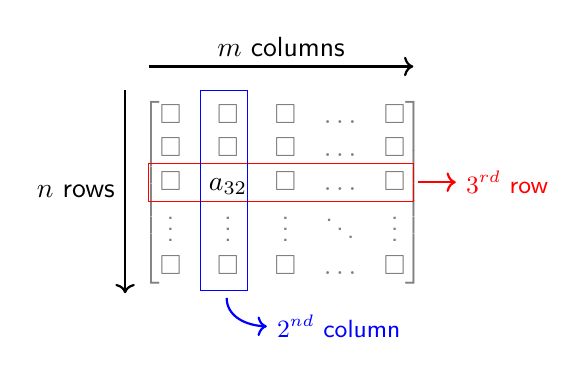
\begin{tikzpicture}[scale=0.6]
\draw[thick, ->] (0,0) -- (0, -4.3) node[midway,left] {$n$ rows};
\draw[thick, ->] (0.5,0.5) -- (6.1, 0.5) node[midway,above]{$m$ columns};
%\node[xshift=-0.6cm,yshift=-1.3cm] {Rows};
\node[gray,xshift=2.0cm,yshift=-1.3cm] {$\begin{bmatrix}
\Box & \Box & \Box & \ldots & \Box \\
\Box & \Box & \Box & \ldots & \Box \\
\Box & \textcolor{black}{a_{32}} & \Box & \ldots & \Box \\
\vdots & \vdots & \vdots & \ddots & \vdots \\
\Box & \Box & \Box & \ldots & \Box \\
\end{bmatrix}$};
\draw[draw=red] (0.5,-2.35) rectangle ++(5.6,0.8);
\draw[draw=blue] (1.6,-4.25) rectangle ++(1.0,4.25);
\draw [thick, blue, ->] (2.15,-4.4) to [out=-90,in=180] (3.0, -5.0) node[right] {\small{$2^{nd}$ column}};
\draw [thick, red, ->] (6.2,-1.95) to (7.,-1.95) node[right] {\small{$3^{rd}$ row}};
\end{tikzpicture}\hspace{0.5cm}
\end{center}
\item Consider a matrix $A$ with $n$ rows and $m$ columns.$ \begin{cases} \text{\textbf{Tall/Skinny}} & n > m\\
\text{\textbf{Square}} & n = m\\
\text{\textbf{Wide/Fat}} & n < m\\
\end{cases}$
\end{itemize}
\end{frame}

\begin{frame}[t]{Matrices}
\begin{itemize}
    \item $n$-vectors can be interpreted as $n \times 1$ matrices. These are called \textit{column vectors}.
    \item A matrix with only one row is called a \textit{row vector}, which can be referred to as $n$-row-vector.  $\mf{x} = \begin{bmatrix}1.45 & -3.1 & 12.4\end{bmatrix}$
    \item\textbf{Block matrices} \& \textbf{Submatrices}: $\mf{A} = \begin{bmatrix}
    \mf{B} & \mf{C} \\
    \mf{D} & \mf{E}
    \end{bmatrix}$.  What are the dimensions of the different matrices?
\end{itemize}
\end{frame}


\begin{frame}[t]{Matrices}
\begin{itemize}
    \item Matrices are also compact way to give a set of indexed column $n$-vectors, 
    $\mf{x}_1, \mf{x}_2, \mf{x}_3 \ldots \mf{x}_m$. 
    $$\mf{X} = \begin{bmatrix}
    \mf{x}_1 & \mf{x}_2 & \mf{x}_3 & \ldots & \mf{x}_m
    \end{bmatrix}$$

    \item \textbf{Zero matrix}$ = \mf{0}_{n\times m} = \begin{bmatrix}
    0 & 0 & \ldots & 0\\
    0 & 0 & \ldots & 0\\
    \vdots & \vdots & \ddots & \vdots\\
    0 & 0 & \ldots & 0
    \end{bmatrix}$

    \item \textbf{Identity matrix} is a square $n \times n$ matrix with all zero elements, except the diagonals where all elements are 1.
    $$i_{mn} = \begin{cases}
    1 & m = n\\
    0 & m \neq n
    \end{cases} \,\,\,\,\,\,\,\, \mf{I}_3=\begin{bmatrix}
    1 & 0 & 0\\
    0 & 1 & 0\\
    0 & 0 & 1\\
    \end{bmatrix} = \begin{bmatrix}
    \mf{e}_1 & \mf{e}_2 & \mf{e}_3
    \end{bmatrix}$$
\end{itemize}
\end{frame}


\begin{frame}[t]{Matrices}
\begin{itemize}

\item \textbf{Diagonal matrices} is a square matrix with non-zero elements on its diagonal.
$$\begin{bmatrix}
0.4 & 0 & 0 & 0\\
0 & -11 & 0 & 0\\
0 & 0 & 21 & 0\\
0 & 0 & 0 & 9.3\\
\end{bmatrix} = \text{\textbf{diag}}\left(0.4, -11, 21, 9.3\right)$$
\item \textbf{Triangular matrices}: Are square matrices. \textit{Upper triangular} $a_{ij} = 0, \forall i > j$; \textit{Lower triangular} $a_{ij} = 0, \forall i < j$.
\end{itemize}
\end{frame}

\begin{frame}[t]{Matrix operations: Transpose}
\begin{itemize}
\item \textbf{Transpose} switches the rows and columns of a matrix. $\mf{A}$ is a $n\times m$ matrix, then its transpose is represented by $\mf{A}^{\top}$, which is a $m \times n$ matrix.
\[ \mf{A} = \begin{bmatrix}
a_{11} & a_{12} & a_{13}\\
a_{21} & a_{22} & a_{23}\\
\end{bmatrix} \implies \mf{A}^{\top} = \begin{bmatrix}
a_{11} & a_{21}\\
a_{12} & a_{22}\\
a_{13} & a_{23}\\
\end{bmatrix} \]
Transpose converts between column and row vectors.\\
What is the transpose of a block matrix? $\mf{A} = \begin{bmatrix}
\mf{B} & \mf{C}\\\mf{D} & \mf{E}
\end{bmatrix}$
\end{itemize}
\end{frame}

\begin{frame}[t]{Matrix operations: Matrix Addition}
\begin{itemize}
\item \textbf{Matrix addition} can only be carried out with matrices of same size. Like vectors we perform element wise addition.
\[ \begin{bmatrix}
a_{11} & a_{12}\\
a_{21} & a_{22}\\
\end{bmatrix} + \begin{bmatrix}
b_{11} & b_{12}\\
b_{21} & b_{22}\\
\end{bmatrix} = \begin{bmatrix}
a_{11} + b_{11} & a_{12} + b_{12}\\
a_{21} + b_{21} & a_{22} + b_{22}\\
\end{bmatrix}\]

\item \textbf{Properties of matrix addition}:
\begin{itemize}
\item \textit{Commutative}: $\mf{A} + \mf{B} = \mf{B} + \mf{A}$
\item \textit{Associative}: $\left(\mf{A} + \mf{B}\right) + \mf{C} = \mf{A} + \left(\mf{B} + \mf{C}\right)$
\item \textit{Addition with zero matrix}: $\mf{A} + \mf{0} = \mf{0} + \mf{A} = \mf{A}$
\item \textit{Transpose of sum}: $\left(\mf{A} + \mf{B}\right)^{\top} = \mf{A}^{\top} + \mf{B}^{\top}$
\end{itemize}
\end{itemize}
\end{frame}

\begin{frame}[t]{Matrix operations: Scalar multiplication}
\begin{itemize}
\item \textbf{Scalar multiplication} Each element of the matrix gets multiplied by the scalar.
\[ \alpha \begin{bmatrix}
a_{11} & a_{12}\\
a_{21} & a_{22}\\
\end{bmatrix} = \begin{bmatrix}
\alpha a_{11} & \alpha a_{12} \\
\alpha a_{21} & \alpha a_{22} \\
\end{bmatrix}\]
\item We will mostly only deal with matrices with real entries. Such matrices are elements of the set $\mathbb{R}^{n\times m}$.
\item Given the aforementioned matrix operations and their properties, is $\mathbb{R}^{n\times m}$ a vector space?
\end{itemize}
\end{frame}

\begin{frame}[t]{Matrix operations: Matrix multiplication}
\begin{itemize}
\item A useful multiplication operation can be defined for matrices.
\item It is possible to \textit{multiply} two matrices $\mf{A} \in \mathbb{R}^{n\times p}$ and $\mf{B} \in \mathbb{R}^{p\times m}$ through this \textit{matrix multiplication} procedure.
\item The product matrix $\mf{C} \coloneqq \mf{A}\mf{B} \in \mathbb{R}^{n \times m}$, if the number of columns of $\mf{A}$ is equal to the number of rows of $\mf{B}$.
\[ c_{ij} \coloneqq \sum_{k=1}^{p} a_{ik}b_{kj} \,\,\,\,\, \forall i \in \left\{1, \ldots n\right\}\,\,\, , j \in \left\{1 \ldots m\right\} \]
\end{itemize}
\end{frame}

\begin{frame}[t]{Matrix multiplication}
\begin{itemize}
\item \textit{Inner product} is a special case of matrix multiplication between a \textit{row vector} and a \textit{column vector}.
\[ \mf{x}^{\top}\mf{y} = \begin{bmatrix}
x_1 \\ x_2 \\ \vdots \\x_n
\end{bmatrix}^{\top}\begin{bmatrix}
y_1 \\ y_2 \\ \vdots \\y_n
\end{bmatrix} = \begin{bmatrix}
x_1 & x_2 & \ldots &x_n
\end{bmatrix}\begin{bmatrix}
y_1 \\ y_2 \\ \vdots \\y_n
\end{bmatrix} = \sum_{i=1}^nx_iy_i\]
\end{itemize}
\end{frame}

\begin{frame}[t]{Matrix multiplication: Post-multiplication by a column vector}
\begin{itemize}
\item Consider a matrix $\mf{A} \in \mathbb{R}^{n \times m}$ and a $m$-vector $\mf{x} \in \mathbb{R}^m$. We can multiply $\mf{A}$ and $\mf{x}$ to obtain $\mf{y} = \mf{A}\mf{x} \in \mathbb{R}^n$.
\[ \mf{y} = \begin{bmatrix}
a_{11} & a_{12} & \ldots & a_{1m} \\
a_{21} & a_{22} & \ldots & a_{2m} \\
\vdots & \vdots & \ddots & \vdots \\
a_{n1} & a_{n2} & \ldots & a_{nm} \\
\end{bmatrix}\begin{bmatrix}
x_1\\ x_2 \\ \vdots \\ x_{m}
\end{bmatrix} = \begin{bmatrix}
\sum_{i=1}^ma_{1i}x_i\\ \sum_{i=1}^ma_{2i}x_i \\ \vdots \\ \sum_{i=1}^ma_{ni}x_i
\end{bmatrix} = \sum_{i=1}^mx_i\begin{bmatrix}
a_{1i} \\ a_{2i} \\ \vdots \\ a_{ni}
\end{bmatrix} = \sum_{i=1}^mx_i \mathbf{a}_{i} \]
\item Post-multiplying a matrix $\mf{A}$ by a column vector $\mf{x}$ results in a linear combination of the columns of matrix $\mf{A}$.

\item $\mathbf{x}$ provides the column mixture.
\end{itemize}
\end{frame}

\begin{frame}[t]{Matrix multiplication: Pre-multiplication by a row vector}
\begin{itemize}
\item Let $\mf{x}^{\top} \in \mathbb{R}^{n}$ and $\mf{A} \in \mathbb{R}^{n \times m}$, then $\mf{y} = \mf{x}^{\top}\mf{A}$.
\[ \mf{y} = \begin{bmatrix}
x_1 & \ldots & x_n
\end{bmatrix} \begin{bmatrix}
a_{11} & \ldots & a_{1m} \\
\vdots & \ddots & \vdots \\
a_{n1} & \ldots & a_{nm} \\
\end{bmatrix} = \begin{bmatrix} \sum_{i=1}^{n} x_i a_{i1} & \ldots & \sum_{i=1}^{n} x_i a_{im}
\end{bmatrix} = \sum_{i=1}^n x_i \tilde{\mf{a}}_i^\top \]
where, $\tilde{\mf{a}}_i^\top = \begin{bmatrix}
a_{i1} & \ldots & a_{im}\end{bmatrix}$
\item Pre-multiplying a matrix $\mf{A}$ by a row vector $\mf{x}$ results in a linear combination of the rows of $\mf{A}$.

\item $\mf{x}^\top$ provides the row mixture.
\end{itemize}
\end{frame}

\begin{frame}[t]{Matrix multiplication}
\begin{itemize}
\item Multiplying two matrices $\mf{A} \in \mathbb{R}^{n \times p}$ and $\mf{B} \in \mathbb{R}^{p \times m}$ produces $\mf{C} \in \mathbb{R}^{n \times m}$,
\[ \mf{C} = \mf{A}\mf{B} = \begin{bmatrix}
a_{11} & a_{12} & \ldots & a_{1p} \\
a_{21} & a_{22} & \ldots & a_{2p} \\
\vdots & \vdots & \ddots & \vdots \\
a_{n1} & a_{n2} & \ldots & a_{np} \\
\end{bmatrix} \begin{bmatrix}
b_{11} & b_{12} & \ldots & b_{1m} \\
b_{21} & b_{22} & \ldots & b_{2m} \\
\vdots & \vdots & \ddots & \vdots \\
b_{p1} & b_{p2} & \ldots & b_{pm} \\
\end{bmatrix} = \begin{bmatrix}
c_{11} & c_{12} & \ldots & c_{1m} \\
c_{21} & c_{22} & \ldots & c_{2m} \\
\vdots & \vdots & \ddots & \vdots \\
c_{p1} & c_{n2} & \ldots & c_{nm} \\
\end{bmatrix}\]

\item \textbf{Four interpretations of matrix multiplication.}
\begin{enumerate}
  \item Inner-Product interpretation
  \item Column interpretation
  \item Row interpretation
  \item Outer product interpretation.
\end{enumerate} 
\end{itemize}
\end{frame}

\begin{frame}[t]{Matrix multiplication: Inner-product Interpreation}
\[ \mf{C} = \mf{A}\mf{B}, \,\,\, \mf{A} \in \mathbb{R}^{n \times p}, \, \mf{B} \in \mathbb{R}^{p \times m}, \, \mf{C} \in \mathbb{R}^{n \times m} \]
\begin{itemize}
\item $ij^{th}$ element of $\mf{C}$ is the inner product of the $i^{th}$ row of $\mf{A}$ and the $j^{th}$ column of $\mf{B}$.
 \[ c_{ij} = \sum_{k=1}^{m} a_{ik} b_{kj} = \tilde{\mf{a}}_i^{\top}\mf{b}_j \]
 where, $i \in \left\{1 \ldots n\right\}, j \in \left\{1 \ldots m\right\}$
\end{itemize}
\end{frame}


\begin{frame}[t]{Matrix multiplication: Column interpretation}
\[ \mf{C} = \mf{A}\mf{B}, \,\,\, \mf{A} \in \mathbb{R}^{n \times p}, \, \mf{B} \in \mathbb{R}^{p \times m}, \, \mf{C} \in \mathbb{R}^{n \times m} \]
\begin{itemize}
\item Columns of $\mf{C}$ are the linear combinations of the columns of $\mf{A}$.
\[ \mf{C} = \mf{A} \begin{bmatrix}
\mf{b}_{1} & \mf{b}_{2} & \ldots & \mf{b}_{m}
\end{bmatrix} = \begin{bmatrix}
\mf{A}\mf{b}_{1} & \mf{A}\mf{b}_{2} & \ldots & \mf{A}\mf{b}_{m}
\end{bmatrix} \]

\item $j^{th}$ column of $\mf{C}$ is the linear combination of the columns of $\mf{A}$
\[ \mf{c}_j = \sum_{k=1}^{p} b_{kj} \mf{a}_k \]
\end{itemize}
\end{frame}


\begin{frame}[t]{Matrix multiplication: Row interpretation}
\[ \mf{C} = \mf{A}\mf{B}, \,\,\, \mf{A} \in \mathbb{R}^{n \times p}, \, \mf{B} \in \mathbb{R}^{p \times m}, \, \mf{C} \in \mathbb{R}^{n \times m} \]
\begin{itemize}
\item Rows of $\mf{C}$ are the linear combinations of the rows of $\mf{B}$.
\[ \mf{C} = \begin{bmatrix}
\tilde{\mf{a}}_{1}^\top \\ \tilde{\mf{a}}_{2}^\top \\ \ldots \\ \tilde{\mf{a}}_{n}^\top
\end{bmatrix} \mf{B}  = \begin{bmatrix}
\tilde{\mf{a}}_{1}^\top \mf{B} \\ \tilde{\mf{a}}_{2}^\top \mf{B} \\ \ldots \\ \tilde{\mf{a}}_{n}^\top \mf{B}
\end{bmatrix} \]

\item $i^{th}$ row of $\mf{C}$ is the linear combination of the rows of $\mf{B}$
\[ \tilde{\mf{c}}_i^\top = \sum_{k=1}^{p} a_{ik} \tilde{\mf{b}}_{k}^\top  \]
\end{itemize}
\end{frame}


\begin{frame}[t]{Matrix multiplication: Outer product interpretation}
\begin{itemize}
    \item \textbf{Outer product}: Product between a colum vector and a row vector. Let $\mf{x} \in \mathbb{R}^n$ and $\mf{y} \in \mathbb{R}^m$. The \textit{outer product} is defined as,
    \[ \mf{x}\mf{y}^{\top} = \begin{bmatrix}
    x_1\\ x_2\\ \vdots \\x_n
    \end{bmatrix} \begin{bmatrix}
    y_1 &  y_2 & \ldots & y_m
    \end{bmatrix} = \begin{bmatrix}
    x_1y_1 &  x_1y_2 & \ldots & x_1y_m \\
    x_2y_1 &  x_2y_2 & \ldots & x_2y_m \\
    \vdots &  \vdots & \ddots & \vdots \\
    x_ny_1 &  x_ny_2 & \ldots & x_ny_m \\
    \end{bmatrix} \in \mb{R}^{n \times m} \]
\end{itemize}
\end{frame}


\begin{frame}[t]{Matrix multiplication: Outer product interpretation}
\[ \mf{C} = \mf{A}\mf{B}, \,\,\, \mf{A} \in \mathbb{R}^{n \times p}, \, \mf{B} \in \mathbb{R}^{p \times m}, \, \mf{C} \in \mathbb{R}^{n \times m} \]
\begin{itemize}
    \item $\mf{C}$ can be written as the sum of $p$ outer products of columns of $\mf{A}$ and rows of $\mf{B}$.
    \[ \mf{C} = \mf{A}\mf{B} = \begin{bmatrix}
    \mf{a}_1 & \mf{a}_2 & \mf{a}_3 & \ldots & \mf{a}_p
    \end{bmatrix} \begin{bmatrix}
    \tilde{\mf{b}}_1^{\top} \\
    \tilde{\mf{b}}_2^{\top} \\
    \tilde{\mf{b}}_3^{\top} \\
    \vdots \\
    \tilde{\mf{b}}_p^{\top}
    \end{bmatrix} = \sum_{i=1}^{p}\mf{a}_i\tilde{\mf{b}}_i^{\top} \]
\end{itemize}
\end{frame}


\begin{frame}[t]{Properties of matrix multiplication}
\begin{itemize}
\item \textbf{Not commutative}: $\mf{A}\mf{B} \neq \mf{B}\mf{A}$\\
The product of two matrices might not alwasys be defined. When it is defined, $\mf{A}\mf{B}$ and $\mf{B}\mf{A}$ need not match.
\item \textbf{Distributive}:  $\mf{A}\left(\mf{B} + \mf{C}\right) = \mf{A}\mf{B} + \mf{B}\mf{C}$ and $\left(\mf{A} + \mf{B}\right)\mf{C} = \mf{A}\mf{C} + \mf{B}\mf{C}$ 
\item \textbf{Associative}: $\mf{A}\left(\mf{B}\mf{C}\right) = \left(\mf{A}\mf{B}\right)\mf{C} $
\item \textbf{Transpose}: $\left(\mf{A}\mf{B}\right)^{\top} = \mf{B}^{\top}\mf{A}^{\top}$
\item \textbf{Scalar product}: $\alpha\left(\mf{A}\mf{B}\right) = \left(\alpha \mf{A}\right)\mf{B} = \mf{A}\left(\alpha \mf{B}\right)$
\end{itemize}
\end{frame}

\begin{frame}[t]{Linear equations}
\begin{itemize}
\item Matrices present a compact way to represent a set of linear equations. Consider the following,
\[
\begin{rcases*}
\begin{split}
a_{11}x_1 + a_{12}x_2 \ldots + a_{1m}x_m & = b_1 \\
a_{21}x_1 + a_{22}x_2 \ldots + a_{2m}x_m & = b_2 \\
a_{31}x_1 + a_{32}x_2 \ldots + a_{3m}x_m & = b_3 \\
\vdots \\
a_{n1}x_1 + a_{n2}x_2 \ldots + a_{nm}x_m & = b_n \\
\end{split}
\end{rcases*} \, \longrightarrow \mf{Ax} = \mf{b}, \,\,\, \mf{A} \in \mathbb{R}^{n \times m}, \,\, \mf{x} \in \mathbb{R}^n, \,\, \mf{b} \in \mathbb{R}^m
\]

\[
\mf{A} = \begin{bmatrix}
a_{11} & a_{12} & a_{13} & \ldots & a_{1m}\\
a_{21} & a_{22} & a_{23} & \ldots & a_{2m}\\
\vdots & \vdots & \vdots & \ddots & \vdots\\
a_{n1} & a_{n2} & a_{n3} & \ldots & a_{nm}\\
\end{bmatrix} \,\,\,\,\, 
\mf{x} = \begin{bmatrix}
x_1\\ x_2\\ \vdots \\ x_m
\end{bmatrix} \,\,\,\,\,
\mf{b} = \begin{bmatrix}
b_1\\ b_2\\ \vdots \\ b_n
\end{bmatrix}
\]
\end{itemize}
\end{frame}


\begin{frame}[t]{Linear equations in control problems}
\begin{LARGE}
\[ \mf{x}: \text{Input} \,\,\, \mf{b}: \text{Output} \,\,\, \mf{A}: \text{System dynamics} \]

\[ \begin{bmatrix}
b_1\\ b_2\\ \vdots \\ b_n
\end{bmatrix} = \begin{bmatrix}
a_{11} & a_{12} & a_{13} & \ldots & a_{1m}\\
a_{21} & a_{22} & a_{23} & \ldots & a_{2m}\\
\vdots & \vdots & \vdots & \ddots & \vdots\\
a_{n1} & a_{n2} & a_{n3} & \ldots & a_{nm}\\
\end{bmatrix} \,\, \begin{bmatrix}
x_1\\ x_2\\ \vdots \\ x_m
\end{bmatrix} \]
\end{LARGE}
\end{frame}

\begin{frame}
\end{frame}


\begin{frame}[t]{Linear equations in estimation problems}
\begin{LARGE}
\[ \mf{x}: \text{Parameter} \,\,\, \mf{b}: \text{Measurements} \,\,\, \mf{A}: \text{System characteristics} \]

\[ \begin{bmatrix}
b_1\\ b_2\\ \vdots \\ b_n
\end{bmatrix} = \begin{bmatrix}
a_{11} & a_{12} & a_{13} & \ldots & a_{1m}\\
a_{21} & a_{22} & a_{23} & \ldots & a_{2m}\\
\vdots & \vdots & \vdots & \ddots & \vdots\\
a_{n1} & a_{n2} & a_{n3} & \ldots & a_{nm}\\
\end{bmatrix} \,\, \begin{bmatrix}
x_1\\ x_2\\ \vdots \\ x_m
\end{bmatrix} \]
\end{LARGE}
\end{frame}


\begin{frame}
\end{frame}


\begin{frame}[t]{Rank of a matrix $\mf{A}$}
\begin{itemize}
\item \textbf{Rank of a matrix $\mf{A}$}: dimension of the subspace spanned by the columns of $\mf{A}$ or the rows of $\mf{A} \in \mb{R}^{n \times m}$. 
\[ \begin{split} 
rank\lp \mf{A} \rp &= \mathrm{dim} \, span\lp \lc \mf{a}_1, \mf{a}_2, \ldots \mf{a}_m \rc \rp \rightarrow \text{Column rank}\\ 
&= \mathrm{dim} \, span\lp \lc \tilde{\mf{a}}_1^\top, \tilde{\mf{a}}_2^\top, \ldots \tilde{\mf{a}}_n^\top \rc \rp \rightarrow \text{Row rank}
\end{split}
\]

\item Column Rank is always equal to the row rank.

\item Rank tells us the number of independent columns/row in the matrix.

\item \textbf{Full rank matrix } $\mf{A}$: $rank\lp \mf{A} \rp  = \min\lp n, m\rp$\\
      \textbf{Rank deficient matrix } $\mf{A}$: $rank\lp \mf{A} \rp  < \min\lp n, m\rp$
\end{itemize}
\end{frame}


\begin{frame}[t]{Geometry of linear equations}
\vspace{-0.5cm}
\[\begin{rcases*}
\begin{split} x_1 + 2x_2 &= -1 \\ x_1 + x_2 &= 1 \end{split}
\end{rcases*} \longrightarrow \bmx
1 & 2\\
1 & 1
\emx \bmx
x_1\\
x_2
\emx = \bmx
-1\\
1
\emx\]
Two ways to view this: \textbf{row view} and the \textbf{column view}.
\begin{center}
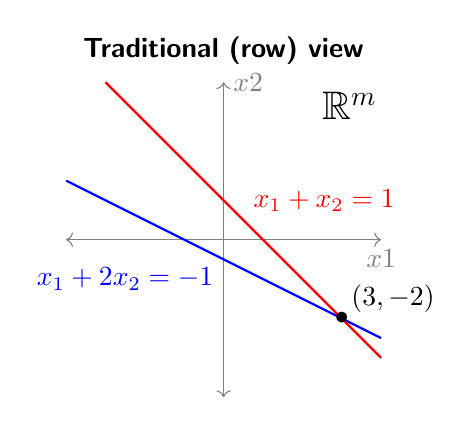
\begin{tikzpicture}[scale=0.5]
\node(0, 0) [yshift=2.4cm] {\textbf{Traditional (row) view}};
\node(0, 0) [xshift=1.6cm,yshift=1.7cm] {\Large {$\mb{R}^m$}};
\draw[gray,<->] (-4, 0) -- (4, 0) node[right,below] {$x1$};
\draw[gray,<->] (0, -4) -- (0, 4) node[right] {$x2$};
\draw[blue,thick] (-4,3/2) -- (4, -5/2) node[midway,left,yshift=-0.25cm] {$x_1 + 2x_2 = -1$};
\draw[red,thick] (-3,4) -- (4, -3) node[midway,right,yshift=0.25cm] {$x_1 + x_2 = 1$};
\draw (3,-2) node[] {$\bullet$};
\draw (3,-2) node[right,yshift=0.25cm] {$\left(3,-2\right)$};
\end{tikzpicture}\hspace{1cm}
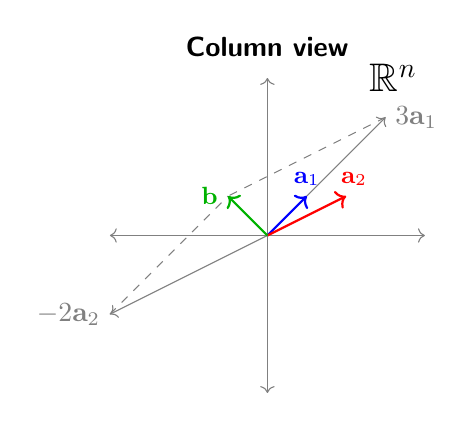
\begin{tikzpicture}[scale=0.5]
\node(0, 0) [yshift=2.4cm] {\textbf{Column view}};
\node(0, 0) [xshift=1.6cm,yshift=2.0cm] {\Large {$\mb{R}^n$}};
\draw[gray,<->] (-4, 0) -- (4, 0);
\draw[gray,<->] (0, -4) -- (0, 4);
\draw[gray,thin,->] (0,0) -- (3,3) node[above,right] {$3\mf{a}_1$};
\draw[blue,thick,->] (0,0) -- (1,1) node[above,yshift=0.cm] {\small{$\mf{a}_1$}};
\draw[red,thick,->] (0,0) -- (2,1) node[above,xshift=0.1cm,yshift=0.cm] {\small{$\mf{a}_2$}};
\draw[gray,thin,->] (0,0) -- (-4,-2) node[below,left] {$-2\mf{a}_2$};
\draw[gray,thin,dashed] (3,3) -- (-1,1);
\draw[gray,thin,dashed] (-4,-2) -- (-1,1);
\draw[black!30!green,thick,->] (0,0) -- (-1,1) node[above,left] {\small{$\mf{b}$}};
\end{tikzpicture}
\end{center}
\end{frame}

\begin{frame}[t]{Solutions of linear equations}
\vspace{-0.5cm}
$$ \mf{Ax = b}, \,\,\, \mf{A} \in \mathbb{R}^{m \times n}, \,\, \mf{x} \in \mathbb{R}^n, \,\, \mf{b} \in \mathbb{R}^m$$
\vspace{-0.5cm}
\begin{itemize}
\item \textbf{Three possible situations:} \textsc{No solution}, \textsc{Infinitely many solutions}, or \textsc{Unique Solution}.
\item When do have infinitely many or no solutions? In $\mathbb{R}^3$, we can visualize the different situations.
\end{itemize}
\begin{center}
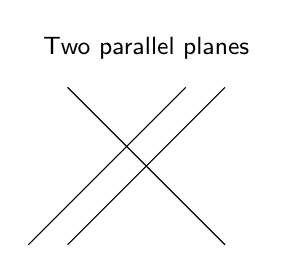
\begin{tikzpicture}[scale=0.5]
\node[yshift=1.5cm] {\small{Two parallel planes}};
\draw[black,-] (-2, -2) -- (2, 2);
\draw[black,-] (-3, -2) -- (1, 2);
\draw[black,-] (2, -2) -- (-2, 2);
\end{tikzpicture}\hspace{0.25cm}
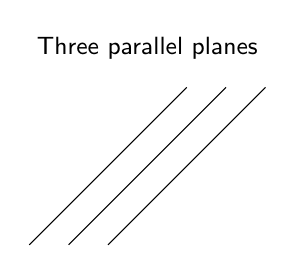
\begin{tikzpicture}[scale=0.5]
\node[yshift=1.5cm] {\small{Three parallel planes}};
\draw[black,-] (-2, -2) -- (2, 2);
\draw[black,-] (-3, -2) -- (1, 2);
\draw[black,-] (-1, -2) -- (3, 2);
\end{tikzpicture}\hspace{0.25cm}
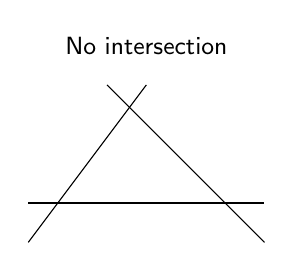
\begin{tikzpicture}[scale=0.5]
\node[yshift=1.0cm] {\small{No intersection}};
\draw[black,-] (-3, -2) -- (3, -2);
\draw[black,-] (-3, -3) -- (0, 1);
\draw[black,-] (3, -3) -- (-1, 1);
\end{tikzpicture}\hspace{0.25cm}
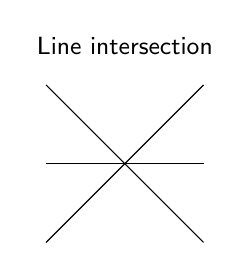
\begin{tikzpicture}[scale=0.5]
\node[yshift=1.5cm] {\small{Line intersection}};
\draw[black,-] (-2, 0) -- (2, 0);
\draw[black,-] (-2, -2) -- (2, 2);
\draw[black,-] (2, -2) -- (-2, 2);
\end{tikzpicture}
\end{center} 
\end{frame}


\begin{frame}[t]{Understanding $\mf{A}\mf{x} = \mf{b}$: Unique solution}

\begin{columns}[t]
\begin{column}{0.3\textwidth}
\[ \bmx
1 & 2\\
1 & 1
\emx\bmx
x_1\\
x_2
\emx = \bmx
-1\\
1
\emx \]
\begin{center}
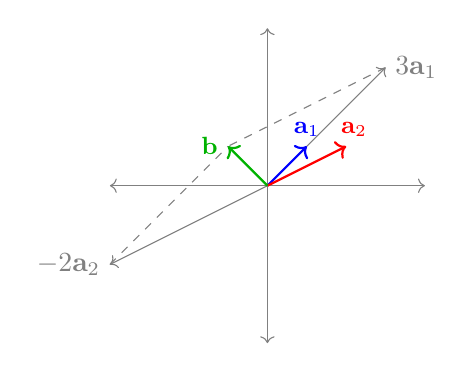
\begin{tikzpicture}[scale=0.5]
\draw[gray,<->] (-4, 0) -- (4, 0);
\draw[gray,<->] (0, -4) -- (0, 4);
\draw[gray,thin,->] (0,0) -- (3,3) node[above,right] {$3\mf{a}_1$};
\draw[blue,thick,->] (0,0) -- (1,1) node[above,yshift=0.cm] {\small{$\mf{a}_1$}};
\draw[red,thick,->] (0,0) -- (2,1) node[above,xshift=0.1cm,yshift=0.cm] {\small{$\mf{a}_2$}};
\draw[gray,thin,->] (0,0) -- (-4,-2) node[below,left] {$-2\mf{a}_2$};
\draw[gray,thin,dashed] (3,3) -- (-1,1);
\draw[gray,thin,dashed] (-4,-2) -- (-1,1);
\draw[black!30!green,thick,->] (0,0) -- (-1,1) node[above,left] {\small{$\mf{b}$}};
\end{tikzpicture}
\end{center}
\end{column}
\hspace{0.5cm}
\begin{column}{0.6\textwidth}
\begin{itemize}
  \item Square matrix
  \item Linearly independent set of columns $\lc \mf{a}_1, \mf{a}_2 \rc$
  \item $\mf{b} \in span\lp{\lc \mf{a}_1, \mf{a}_2 \rc}\rp$.
  \item Always solvable, and give an unique solution.
\end{itemize}
\end{column}
\end{columns}
\end{frame}


\begin{frame}[t]{Understanding $\mf{A}\mf{x} = \mf{b}$: Unique solution or No solution}
\begin{columns}[t]
\begin{column}{0.3\textwidth}
\begin{enumerate}
  \item $\bmx 2\\ 1 \emx \bmx x_1 \emx = \mf{b}_1 = \bmx -1\\ 1 \emx$
  \item $\bmx 2\\ 1 \emx \bmx x_1 \emx = \mf{b}_2 = \bmx 3\\ 1.5 \emx$
\end{enumerate}

\begin{center}
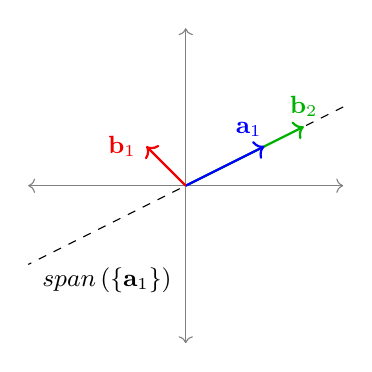
\begin{tikzpicture}[scale=0.5]
\draw[gray,<->] (-4, 0) -- (4, 0);
\draw[gray,<->] (0, -4) -- (0, 4);
\draw[black,dashed] (4, 2) -- (-4,-2) node[xshift=1cm,,yshift=-0.2cm] {\small{$span\lp \lc \mf{a}_1 \rc\rp$}};
\draw[black!30!green,thick,->] (0,0) -- (3,1.5) node[above,xshift=0.0cm,yshift=0.cm] {\small{$\mf{b}_2$}};
\draw[blue,thick,->] (0,0) -- (2,1) node[above,xshift=-0.2cm,yshift=0.cm] {\small{$\mf{a}_1$}};
% \draw[gray,thin,dashed] (3,3) -- (-1,1);
% \draw[gray,thin,dashed] (-4,-2) -- (-1,1);
\draw[black!5!red,thick,->] (0,0) -- (-1,1) node[above,left] {\small{$\mf{b}_1$}};
\end{tikzpicture}
\end{center}
\end{column}
\hspace{0.5cm}
\begin{column}{0.6\textwidth}
\begin{itemize}
  \item Tall matrix
  \item Linearly independent set of columns $\lc \mf{a}_1 \rc$
\end{itemize}
\vspace{0.25cm}
$\mf{b}_1 \notin span\lp{\lc \mf{a}_1 \rc}\rp \implies$ Not solvable.

\vspace{0.25cm}
$\mf{b}_2 \in span\lp{\lc \mf{a}_1 \rc}\rp \implies$ Solvable with unqiue solution.
\end{column}
\end{columns}
\end{frame}


\begin{frame}[t]{Understanding $\mf{A}\mf{x} = \mf{b}$: Infinitely many solution}
\begin{columns}[t]
\begin{column}{0.3\textwidth}
\[ \bmx
1 & 2 & -1\\
1 & 1 & -2
\emx\bmx
x_1\\
x_2\\
x_3
\emx = \bmx
-1\\
1
\emx \]
\begin{center}
\begin{tikzpicture}[scale=0.5]
\draw[gray,<->] (-4, 0) -- (4, 0);
\draw[gray,<->] (0, -4) -- (0, 4);
% \draw[gray,thin,->] (0,0) -- (3,3) node[above,right] {$3a_1$};
\draw[blue,thick,->] (0,0) -- (1,1) node[above,yshift=0.cm] {\small{$\mf{a}_1$}};
\draw[red,thick,->] (0,0) -- (2,1) node[above,xshift=0.1cm,yshift=0.cm] {\small{$\mf{a}_2$}};
\draw[black!30!green,thick,->] (0,0) -- (-1,-2) node[above,xshift=0cm,yshift=-0.4cm] {\small{$\mf{a}_3$}};
\draw[black,thick,->] (0,0) -- (-1,1) node[above,left] {\small{$b$}};
\end{tikzpicture}
\end{center}
\end{column}
\hspace{0.5cm}
\begin{column}{0.6\textwidth}
\begin{itemize}
  \item Fat matrix
  \item Linearly dependent set of columns $\lc \mf{a}_1, \mf{a}_2, \mf{a}_3 \rc$
  \item $\mf{b} \in span\lp{\lc \mf{a}_1, \mf{a}_2, \mf{a}_3 \rc}\rp$.
  \item Always solvable, with infinitely many solutions.
\end{itemize}
\end{column}
\end{columns}
\end{frame}


\begin{frame}[t]{Understanding $\mf{A}\mf{x} = \mf{b}$: Conditions for different types of solutions}
\[ \mf{A}\mf{x} = \mf{b}, \,\,\, \mf{A} \in \mb{R}^{n \times m}, \, \mf{x} = \mb{R}^m, \, \mf{b} \in \mb{R}^n \]

\textbf{Full rank } $\mf{A}$:
\begin{itemize}
  \item $rank\lp \mf{A} \rp = n \implies$ \textbf{Always solvable}\\
        \vspace{0.2cm}
        $\begin{cases} 
        n = m & \implies \text{Unique solution} \\ 
        n < m & \implies \text{Infinitely many solutions} \\ 
        \end{cases}$
  \item $rank\lp \mf{A} \rp = m  \implies$ \textbf{No infinite solutions}\\
        \vspace{0.2cm}
        $\begin{cases} 
        m = n & \implies \text{Unique solution} \\ 
        m < n & \rightarrow \begin{cases}
        \mf{b} \in span\lp \mf{a}_1, \ldots \mf{a}_m \rp {\implies} \text{Unique solution} \\
        \mf{b} \notin span\lp \mf{a}_1, \ldots \mf{a}_m \rp {\implies} \text{No solution}
        \end{cases}\\ 
        \end{cases}$
\end{itemize}
\end{frame}


\begin{frame}[t]{Understanding $\mf{A}\mf{x} = \mf{b}$: Conditions for different types of solutions}
\[ \mf{A}\mf{x} = \mf{b}, \,\,\, \mf{A} \in \mb{R}^{n \times m}, \, \mf{x} = \mb{R}^m, \, \mf{b} \in \mb{R}^n \]

\textbf{Rank deficient} $\mf{A}$:
\begin{itemize}
  \item $rank\lp \mf{A} \rp < \min \lp n, m \rp \implies$ \textbf{No unique solution}\\
        \vspace{0.2cm}
        $\begin{cases}
        \mf{b} \in span\lp \mf{a}_1, \ldots \mf{a}_m \rp {\implies} \text{Infinitely many solutions} \\
        \mf{b} \notin span\lp \mf{a}_1, \ldots \mf{a}_m \rp {\implies} \text{No solution}
        \end{cases}$
\end{itemize}
\end{frame}


\begin{frame}[t]{Understanding $\mf{A}\mf{x} = \mf{b}$: Conditions for different types of solutions}
\[ \mf{A}\mf{x} = \mf{b}, \,\,\, \mf{A} \in \mb{R}^{n \times m}, \, \mf{x} = \mb{R}^m, \, \mf{b} \in \mb{R}^n \]
\vspace{0.5cm}
\begin{itemize}
  \item $\mf{b} \notin span\lp \mf{a}_1, \ldots \mf{a}_m \rp {\implies} \text{No solution}$
  \vspace{-2cm}
  \item $\mf{b} \in span\lp \mf{a}_1, \ldots \mf{a}_m \rp {\implies} \begin{cases}
        rank\lp \mf{A} \rp = m \implies \text{Unique} \\
        rank\lp \mf{A} \rp < m \implies \text{Infinitely many solutions}
        \end{cases}$
\end{itemize}
\end{frame}

\begin{frame}[t]{General solution of linear equations}
\[ \mf{A}\mf{x} = \mf{b}, \,\,\, \mf{A} \in \mb{R}^{n \times m}, \, \mf{x} = \mb{R}^m, \, \mf{b} \in \mb{R}^n \]

\begin{itemize}
  \item Assuming that this system can be solved, the most general form of the solution is,
  \[ \mf{x} = \mf{x}_p + \mf{x}_h \]
  where, $\mf{x}_p$ is called the particular solution, and $\mf{x}_h$ is the homogenous solution.

  \item \textbf{Homogenous solution}: Solution of the equation $\mf{A}\mf{x} = \mf{0}$.

  \item The set of all homogenous solutions of $\mf{A}$ -- $\lc \mf{x}_h \, \vert \, \mf{A}\mf{x}_h = \mf{0} \rc$ -- form a subspace of $\mb{R}^m$.
\end{itemize}
\end{frame}

\begin{frame}[t]{Geometry of the general solution}
\[ \mf{A}\mf{x} = \mf{b}, \,\,\, \mf{A} \in \mb{R}^{n \times m}, \, \mf{x} = \mb{R}^m, \, \mf{b} \in \mb{R}^n \]
\begin{columns}[t]
\begin{column}{0.3\textwidth}
\[ \mf{A} = \bmx
1 & -1\\
2 & -2
\emx, \,\, \mf{b} = \bmx
1.5\\
3
\emx \]
\end{column}
\hspace{0.5cm}
\begin{column}{0.6\textwidth}
\end{column}
\end{columns}
\end{frame}

\begin{frame}[t]{Geometry of the general solution}
\begin{center}
\vspace{-0.2cm}
\begin{small}
$\mf{A} = \bmx
1 &  2\\
1 &  1
\emx, \,\, \mf{b} = \bmx
-1\\
1
\emx$
\end{small}
\vspace{0.5cm}

\begin{tikzpicture}[scale=0.45]
\node[] at (-5, 5) {\Large $\mb{R}^m$};
\draw[gray,<->] (-6, 0) -- (6, 0) node[right,below] {$x_1$};
\draw[gray,<->] (0, -6) -- (0, 6) node[right] {$x_2$};
\draw[black,thick,->] (0,0) -- (3,-2);
\node[above] at (3, -2) {$\mf{x}_p$};
\node[black!30!green,above left] at (0, 0) {\small $\mf{x}_h = \mf{0}$};

\node[] at (-5 + 14, 5) {\Large $\mb{R}^n$};
\draw[gray,<->] (-6 + 14, 0) -- (6 + 14, 0);
\draw[gray,<->] (0 + 14, -6) -- (0 + 14, 6);
% \node[above, xshift=-0.5cm]  at (-3.2 + 14, -4) {\small $span\lp \lc \mf{a}_1, \mf{a}_2 \rc \rp$};
% \draw[black!30!green,thick,->] (0 + 14,0) -- (2 + 14,4) node[above,right] {$\mf{b}$};
\draw[red,thick,->] (0 + 14,0) -- (1 + 14,1) node[xshift=-0.1cm,above] {\small $\mf{a}_1$};
\draw[blue,thick,->] (0 + 14,0) -- (2 + 14,1) node[below,yshift=-0.05cm] {\small{$\mf{a}_2$}};
\draw[red,thin,dashed] (-6 + 14,-6) -- (6 + 14,6);
\node[red, rotate=45] at (3 + 14, 3.9) {\small $span\lp\lc \mf{a}_1 \rc\rp$};
\draw[blue,thin,dashed] (-6 + 14,-3) -- (6 + 14,3);
\node[blue, rotate=26.6] at (4.5 + 14, 1.6) {\small $span\lp\lc \mf{a}_2 \rc\rp$};
\draw[black!30!green,thick,->] (0 + 14,0) -- (-1 + 14,1);
\node[above left] at (-1, 1) {\small $\mf{b}$};
\draw[red, thin, -latex] (3+0.1, -2) to[out=30,in=-135] (-1 + 14 - 0.1, 1);
\node[] at (7, -1.5) {$\mf{A}$};
\end{tikzpicture}
\end{center}
\end{frame}


\begin{frame}[t]{Geometry of the general solution}
\begin{center}
\vspace{-0.2cm}
\begin{small}
$\mf{A} = \bmx
2\\
1
\emx, \,\, \mf{b} = \bmx
-4\\
-2
\emx$
\end{small}
\vspace{0.5cm}

\begin{tikzpicture}[scale=0.45]
\node[] at (-5, 5) {\Large $\mb{R}^m$};
\draw[gray,<->] (-6, 0) -- (6, 0) node[right,below] {$x_1$};
\draw[black,thick,->] (0,0) -- (-2,0);
\node[above left] at (-2, 0) {$\mf{x}_p$};
\node[black!30!green,below] at (0, 0) {\small $\mf{x}_h = \mf{0}$};

\node[] at (-5 + 14, 5) {\Large $\mb{R}^n$};
\draw[gray,<->] (-6 + 14, 0) -- (6 + 14, 0);
\draw[gray,<->] (0 + 14, -6) -- (0 + 14, 6);
\draw[blue,thick,->] (0 + 14,0) -- (2 + 14,1) node[below,yshift=-0.05cm] {\small{$\mf{a}_1$}};
\draw[blue,thin,dashed] (-6 + 14,-3) -- (6 + 14,3);
\node[blue, rotate=26.6] at (4.5 + 14, 1.6) {\small $span\lp\lc \mf{a}_1 \rc\rp$};
\draw[black!30!green,thick,->] (0 + 14,0) -- (-4 + 14,-2);
\node[above left] at (-4 + 14, -2) {\small $\mf{b}$};
\draw[red, thin, -latex] (-2, 0 - 0.1) to[out=-90,in=-100] (-4 + 14, -2);
\node[] at (5, -4) {$\mf{A}$};
\end{tikzpicture}
\end{center}
\end{frame}


\begin{frame}[t]{Geometry of the general solution}
\begin{center}
\vspace{-0.2cm}
\begin{small}
$\mf{A} = \bmx
2 &  1
\emx, \,\, \mf{b} = \bmx
5
\emx$
\end{small}
\vspace{0.5cm}


\begin{tikzpicture}[scale=0.45]
\node[] at (-5, 5) {\Large $\mb{R}^m$};
\draw[gray,<->] (-6, 0) -- (6, 0) node[right,below] {$x_1$};
\draw[gray,<->] (0, -6) -- (0, 6) node[right] {$x_2$};
\draw[black,thick,->] (0,0) -- (2,1);
\node[] at (1, 1.2) {$\mf{x}_p$};
\draw[black!30!green,thick,dotted] (-3, 6) -- (3,-6);
\node[black!30!green,below,rotate=-63.43] at (3, -3) {\small $\lc \mf{x}_h \, \vert \, \mf{A}\mf{x}_h = \mf{0} \rc$};
\draw[black!30!green,thick] (5.5,-6) -- (-0.5,6);
\node[black!30!green,rotate=-63.43] at (1.2, 4) {\small $\mf{x}_p + \mf{x}_h$};

\node[] at (5 + 14, 5) {\Large $\mb{R}^n$};
\draw[gray,<->] (-6 + 14, 0) -- (6 + 14, 0);
\draw[black,thick,->] (0 + 14,0) -- (5 + 14,0);
\node[below] at (5 + 14, 0) {\msall $\mf{b}$};
% \draw[gray,<->] (0 + 14, -6) -- (0 + 14, 6);
% \draw[black,thick,dashed] (3 + 14,6) -- (-3 + 14,-6);
% \node[above, xshift=-0.5cm]  at (-3.2 + 14, -4) {\small $span\lp \lc \mf{a}_1, \mf{a}_2 \rc \rp$};
% \draw[black!30!green,thick,->] (0 + 14,0) -- (2 + 14,4) node[above,right] {$\mf{b}$};
% \draw[red,thick,->] (0 + 14,0) -- (1 + 14,2) node[above,right] {$\mf{a}_1$};
% \draw[blue,thick,->] (0 + 14,0) -- (-1 + 14,-2) node[above,xshift=-0.25cm] {\small{$\mf{a}_2$}};
\draw[red, thin, -latex] (1.5 + 0.1, 2) to[out=30,in=90] (5 + 14, 0 + 0.1);
\node[] at (9, 5.5) {$\mf{A}$};
\end{tikzpicture}
\end{center}
\end{frame}


\begin{frame}[t]{Geometry of the general solution}
\begin{center}
\vspace{-0.2cm}
\begin{small}
$\mf{A} = \bmx
1 & -1\\
2 & -2
\emx, \,\, \mf{b} = \bmx
2\\
4
\emx$
\end{small}
\vspace{0.5cm}

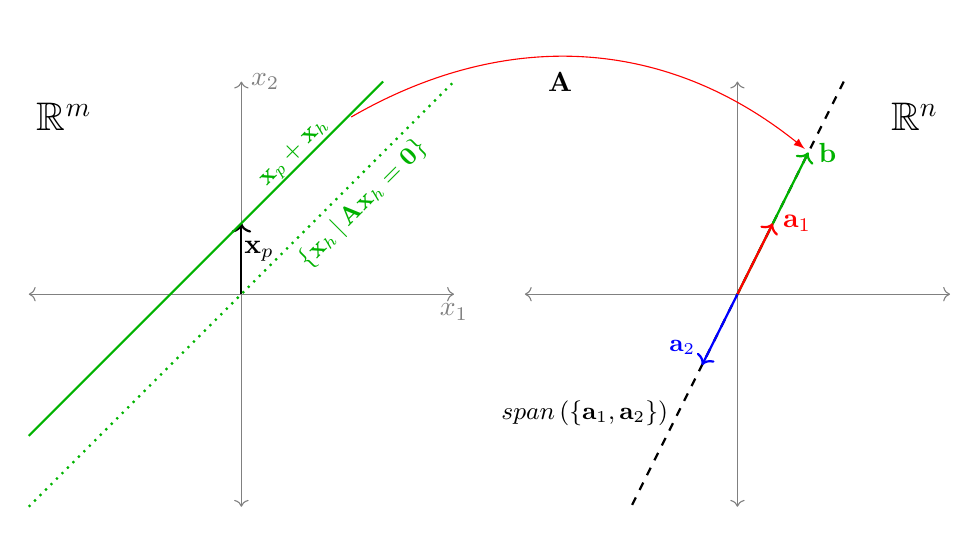
\begin{tikzpicture}[scale=0.45]
\node[] at (-5, 5) {\Large $\mb{R}^m$};
\draw[gray,<->] (-6, 0) -- (6, 0) node[right,below] {$x_1$};
\draw[gray,<->] (0, -6) -- (0, 6) node[right] {$x_2$};
\draw[black,thick,->] (0,0) -- (0,2);
\node[] at (0.5, 1.2) {$\mf{x}_p$};
\draw[black!30!green,thick,dotted] (-6,-6) -- (6,6);
\node[black!30!green,below,rotate=45] at (3, 3) {\small $\lc \mf{x}_h \, \vert \, \mf{A}\mf{x}_h = \mf{0} \rc$};
\draw[black!30!green,thick] (-6,-4) -- (4,6);
\node[black!30!green,rotate=45] at (1.5, 4) {\small $\mf{x}_p + \mf{x}_h$};

\node[] at (5 + 14, 5) {\Large $\mb{R}^n$};
\draw[gray,<->] (-6 + 14, 0) -- (6 + 14, 0);
\draw[gray,<->] (0 + 14, -6) -- (0 + 14, 6);
\draw[black,thick,dashed] (3 + 14,6) -- (-3 + 14,-6);
\node[above, xshift=-0.5cm]  at (-3.2 + 14, -4) {\small $span\lp \lc \mf{a}_1, \mf{a}_2 \rc \rp$};
\draw[black!30!green,thick,->] (0 + 14,0) -- (2 + 14,4) node[above,right] {$\mf{b}$};
\draw[red,thick,->] (0 + 14,0) -- (1 + 14,2) node[above,right] {$\mf{a}_1$};
\draw[blue,thick,->] (0 + 14,0) -- (-1 + 14,-2) node[above,xshift=-0.25cm] {\small{$\mf{a}_2$}};
\draw[red, thin, -latex] (3.1, 5) to[out=30,in=140] (2 + 14 - 0.1, 4 + 0.1);
\node[] at (9, 6) {$\mf{A}$};
\end{tikzpicture}
\end{center}
\end{frame}


\begin{frame}[t]{Linear transformations}
\begin{itemize}
    \item Linear functions $f: \mathbb{R}^m \mapsto \mathbb{R}$, 
    $$y = f\left(\mf{x}\right) = \mf{w}^{\top}\mf{x}; \,\,\, \mf{w}, \mf{x} \in \mathbb{R}^m, \,\, y \in \mathbb{R}$$

    \item Generalization of the linear function is when its range $\mathbb{R}^n$:
    $$\mf{y} = f\left(\mf{x}\right); \,\,\, \mf{x} \in \mathbb{R}^m, \,\, \mf{y} \in \mathbb{R}^n$$

    \item These can be represented as, $\mf{y} = \mf{Ax}, \,\,\, \mf{A} \in \mathbb{R}^{n \times m}$.\\

    \item Matrices can be thought of as representing a particular linear transformation.
\end{itemize}
\end{frame}


\begin{frame}[t]{Why does matrix multiplication have this strange definition?}
Consider the following two functions,
\begin{small}
\[ \mf{y} = f\lp\mf{x}\rp = \mf{A}\mf{x} \longrightarrow \begin{bmatrix}y_1 \\ y_2\end{bmatrix} = f\left(\begin{bmatrix}x_1 \\ x_2\end{bmatrix}\right) = \begin{bmatrix}ax_1 + bx_2 \\ cx_1 + dx_2\end{bmatrix} = \begin{bmatrix}a & b \\ c & d\end{bmatrix}\begin{bmatrix}x_1 \\ x_2\end{bmatrix}\]
\[ \mf{v} = g\lp\mf{u}\rp = \mf{B}\mf{u} \longrightarrow \begin{bmatrix}v_1 \\ v_2\end{bmatrix} = g\left(\begin{bmatrix}u_1 \\ u_2\end{bmatrix}\right) = \begin{bmatrix}\alpha u_1 + \beta u_2 \\ \gamma u_1 + \delta u_2\end{bmatrix} = \begin{bmatrix}\alpha & \beta \\ \gamma & \delta\end{bmatrix}\begin{bmatrix}u_1 \\ u_2\end{bmatrix}\]
\[ \begin{split}
\mf{z} = h\left(\mf{u}\right) &= f\left(g\left(\mf{u}\right)\right) = f\left(\begin{bmatrix}\alpha u_1 + \beta u_2 \\ \gamma u_1 + \delta u_2\end{bmatrix}\right) = \begin{bmatrix}a\alpha u_1 + a\beta u_2 + b\gamma u_1 + b\delta u_2 \\ c\alpha u_1 + c\beta u_2 + d\gamma u_1 + d\delta u_2 \end{bmatrix}\\
&= \begin{bmatrix}\left(a\alpha + b\gamma\right) u_1 + \left(a\beta + b\delta\right)u_2 \\ \left(c\alpha + d\gamma\right)u_1  + \left(c\beta + d\delta\right)u_2 \end{bmatrix} = \begin{bmatrix}a\alpha + b\gamma & a\beta + b\delta \\ c\alpha + d\gamma & c\beta + d\delta \end{bmatrix} \begin{bmatrix}u_1 \\ u_2 \end{bmatrix}
\end{split}
\]
\[\mf{z} = \mf{A}\lp\mf{B}\mf{u}\rp = \lp\mf{A}\mf{B}\rp\mf{u} \implies \mf{A}\mf{B} = \begin{bmatrix}a & b \\ c & d\end{bmatrix}\begin{bmatrix}\alpha & \beta \\ \gamma & \delta\end{bmatrix} = \begin{bmatrix}a\alpha + b\gamma & a\beta + b\delta \\ c\alpha + d\gamma & c\beta + d\delta \end{bmatrix}
\]
\end{small}
Matrix multiplication represents the composition of linear transformations.
\end{frame}


\begin{frame}[t]{Four Fundamental Subspaces of $\mf{A} \in \mb{R}^{n \times m}$}
\begin{itemize}
    \item $\mathcal{C}\left(\mf{A}\right)$: \textbf{Column Space of} $\mf{A}$ -- the span of the columns of $\mf{A}$.
    \[ \mathcal{C}\left(\mf{A}\right) = \left\{\mf{Ax} \left|\right. \mf{x} \in \mathbb{R}^m\right\} \subseteq \mathbb{R}^n \]

    \item $\mathcal{N}\left(\mf{A}\right)$: \textbf{Nullspace of} $\mf{A}$ -- the set of all $\mf{x} \in \mathbb{R}^m$ that are mapped to zero by $\mf{A}$.
    \[ \mathcal{N}\left(\mf{A}\right) = \left\{\mf{x} \left|\right. \mf{Ax}  = \mf{0}\right\} \subseteq \mathbb{R}^m \]
    
    \item $\mathcal{C}\left(\mf{A}^{\top}\right)$: \textbf{Row Space of} $\mf{A}$ -- the span of the rows of $\mf{A}$.
    \[ \mathcal{C}\left(\mf{A}^{\top}\right) = \left\{\mf{A}^{\top}\mf{y} \left|\right. \mf{y} \in \mathbb{R}^n\right\} \subseteq \mathbb{R}^m \]

    \item $\mathcal{N}\left(\mf{A}^{\top}\right)$: \textbf{Nullspace of} $\mf{A}^{\top}$ -- the set of all $\mf{y} \in \mathbb{R}^n$ that are mapped to zero by $\mf{A}^{\top}$.
    \[ \mathcal{N}\left(\mf{A}^{\top}\right) = \left\{\mf{y} \left|\right. \mf{A}^{\top}\mf{y}  = \mf{0}\right\} \subseteq \mathbb{R}^n \]

    This is also called the \textbf{left nullspace} of $\mf{A}$.
\end{itemize}
\end{frame}

\begin{frame}[t]{Linear Independence}
\begin{itemize}
    \item Given a set of vectors $\left\{\mf{v}_1, \mf{v}_2, \ldots \mf{v}_m\right\}, \,\,\, \mf{v}_i \in \mathbb{R}^n$, how can we determine if this set is linear independent?
    \item We need to verify, $a_1 \mf{v}_1 + a_2 \mf{v}_2 + \cdots + a_m \mf{v}_m= 0$
    \[ \begin{rcases*}\begin{bmatrix} \mf{v}_1 & \cdots & \mf{v}_m\end{bmatrix} \begin{bmatrix} a_1 \\ \vdots \\ a_m\end{bmatrix} = \begin{bmatrix} 0 \\ \vdots \\ 0\end{bmatrix} = \mf{V}\mf{a} = \mf{0}\end{rcases*} \mathcal{N}\left(\mf{V}\right) = \left\{\mf{0}\right\}, \,\,\, rank\left(\mf{V}\right) = n  \]
    \item This is also equivalent to saying that when the $rank \left(\mf{A}\right) = n \implies$ the columns of $\mf{A}$ form an independent set of vectors.
    \item When do the rows of $\mf{A}$ form an independent set?
    \item What about both rows and columns? When does that happen?
\end{itemize}
\end{frame}


\begin{frame}[t]{Dimension of the four fundamental subspaces}
\begin{itemize}
    \item \textbf{Column space} $C(\mf{A})$
    \begin{itemize}
        \item $\dim \,C(\mf{A}) = rank\left(\mf{A}\right) = r$
    \end{itemize}
    \item \textbf{Nullspace} $N(\mf{A})$
    \begin{itemize}
        \item $\dim \,N(\mf{A}) = n-r$
    \end{itemize}
    \item \textbf{Row space} $C(\mf{A}^{\top})$
    \begin{itemize}
        \item $\dim \,C(\mf{A}^{\top}) = rank\left(\mf{A}^{\top}\right) = rank\left(\mf{A}\right) = r$
    \end{itemize}
    \item \textbf{Left Nullspace} $N(\mf{A}^{\top})$
    \begin{itemize}
        \item $\dim \,N(\mf{A}^{\top}) = m-r$
    \end{itemize}
\end{itemize}
\end{frame}


\begin{frame}[t]{Matrix Inverse}
\begin{small}
\begin{itemize}
    \item Consider the square matrix $\mf{A} \in \mathbb{R}^{n \times n}$. $\mf{B} \in \mathbb{R}^{n \times n}$ is the inverse of $\mf{A}$, if $\mf{AB} = \mf{BA} = \mf{I}_n$, and $\mf{B}$ is represented as $\mf{A}^{-1}$.
    \item Not all matrices have inverses. A matrix with an inverse is called \textbf{non-singular}, otherwise it is called \textbf{singular}.
    \item For a non-singular matrix $\mf{A}$, $\mf{A}^{-1}$ is unique. $\mf{A}^{-1}$ is both the left and right inverse.
    \item A matrix $\mf{A}$ has an inverse, if and only if $\mf{A}$ is full rank, i.e. $rank\left(\mf{A}\right) = n$
    \item $\mf{Ax} = \mf{b}$ can be solved as follows, $\mf{x} = \mf{A}^{-1}\mf{b}$. \textit{It is never solved like this in practice.}
    \item Inverse of product of matrices, $\left(\mf{AB}\right)^{-1} = \mf{B}^{-1}\mf{A}^{-1}$.
    \item $\left(\mf{A}^{-1}\right)^{-1} = \mf{A}$ and $\left(\mf{A}^{-1}\right)^{\top} = \left(\mathbf{A}^{T}\right)^{-1}$
\end{itemize}
\end{small}
\end{frame}

\end{document}
\documentclass[9pt]{article}

\usepackage[utf8]{inputenc}
\usepackage{geometry}
\geometry{
    a4paper,
    total={170mm,257mm},
    left=15mm,
    right=15mm,
    top=20mm,
    bottom=20mm,
}
\usepackage{multicol}
\usepackage[font=small,labelfont=bf]{caption}
\setlength{\columnsep}{0.25cm}
\usepackage[inline]{enumitem}
\usepackage{amssymb}
\usepackage{xcolor}
\usepackage{mathtools} 
\setlength{\parindent}{0em}
\setlength{\parsep}{0em}
\usepackage{tikz}
\setlength{\parskip}{0em}
\usetikzlibrary{decorations.pathmorphing,patterns}
\usepackage[american,cuteinductors]{circuitikz}
\usetikzlibrary{shapes,arrows,circuits,calc,babel}
% Definition of blocks:
\tikzset{%
  block/.style    = {draw, thick, rectangle, minimum height = 3em,
    minimum width = 3em},
  sum/.style      = {draw, circle, node distance = 2cm}, % Adder
  input/.style    = {coordinate}, % Input
  output/.style   = {coordinate} % Output
}
% Defining string as labels of certain blocks.
\newcommand{\suma}{\Large$+$}
\newcommand{\inte}{$\displaystyle \int$}
\newcommand{\derv}{\huge$\frac{d}{dt}$}

\def\mf{\ensuremath\mathbf}
\def\mb{\ensuremath\mathbb}
\def\mc{\ensuremath\mathcal}
\def\lp{\ensuremath\left(}
\def\rp{\ensuremath\right)}
\def\lv{\ensuremath\left\lvert}
\def\rv{\ensuremath\right\rvert}
\def\lV{\ensuremath\left\lVert}
\def\rV{\ensuremath\right\rVert}
\def\lc{\ensuremath\left\{}
\def\rc{\ensuremath\right\}}
\def\ls{\ensuremath\left[}
\def\rs{\ensuremath\right]}
\def\bmx{\ensuremath\begin{bmatrix*}[r]}
\def\emx{\ensuremath\end{bmatrix*}}
\def\bmxc{\ensuremath\begin{bmatrix*}[c]}
\def\emxc{\ensuremath\end{bmatrix*}}
% \def\t{\lp t\rp}
% \def\k{\ls k\rs}

\newcommand{\demoex}[2]{\onslide<#1->\begin{color}{black!60} #2 \end{color}}
\newcommand{\demoexc}[3]{\onslide<#1->\begin{color}{#2} #3 \end{color}}
\newcommand{\anim}[3]{\onslide<#1->{\begin{color}{#2!60} #3 \end{color}}}
\newcommand{\ct}[1]{\lp #1\rp}
\newcommand{\dt}[1]{\ls #1\rs}

\renewcommand{\familydefault}{\sfdefault}

\begin{document}
\begin{center}
\begin{Large}
\textbf{Linear Systems: Orthogonality Assignment}
\end{Large}
\end{center}
\vspace{0.2cm}

\begin{multicols}{2}
  \begin{enumerate}
    \item Consider an orthonormal set of vectors $V = \left\{ \mf{v}_1, \mf{v}_2, \ldots \mf{v}_r\right\},\,\,\, \mf{v}_i \in \mb{R}^n\,\,\,\forall i \in \left\{1, 2, \ldots r\right\}$. If there is a vector $\mf{w} \in \mb{R}^n$ such that $\mf{v}_i^T\mf{w} = 0\,\,\,\forall i \in \left\{1, 2, \ldots r\right\}$. Prove that $\mf{w} \notin span\left(V\right)$.
    
    \item Consider the following set of vectors in $\mb{R}^4$.
    \[ V = \left\{
    \bmx
    1\\-2\\0\\3
    \emx,
    \bmx
    1\\1\\1\\1
    \emx,
    \bmx
    2\\-1\\1\\4
    \emx
    \right\} \]
    Find the set of all vectors that are orthogonal to $V$?

    \item For a matrix $\mf{A} \in \mb{R}^{m \times n}$, prove that $C\lp\mf{A}\rp \perp N\lp\mf{A}^T\rp$ and $C\lp\mf{A}^T\rp \perp N\lp\mf{A}\rp$.

    \item If the columns of a matrix $\mf{A} \in \mb{R}^{n \times n}$ are orthonormal, prove that $\mf{A}^{-1} = \mf{A}^T$. What is $\mf{A}^T\mf{A}$ when $\mf{A}$ is rectangular $\left(\mf{A} \in \mb{R}^{m \times n}\right)$ with orthonormal columns?

    \item What will happen when the Gram-Schmidt procedure is applied to: (a) orthonormal set of vectors; and (b) orthogonal set of vectors? If the set of vectors are columns of a matrix $\mf{A}$, then what are the corresponding $\mf{Q}$ and $\mf{R}$ matrices for the orthonormal and orthogonal cases?

    \item Consider the linear map, $\mf{y} = \mf{Ax}$, such that $\mf{x}, \mf{y} \in \mb{R}^n$ and $\mf{A} \in \mb{R}^{n \times n}$. Let us assume that $\mf{A}$ is full rank. What conditions must $\mf{A}$ satisfy for the following statements to be true,
    \begin{enumerate}
        \item $\left\lVert \mf{y}\right\rVert_2 = \left\lVert \mf{x}\right\rVert_2$, for all $\mf{x}, \mf{y}$ such that $\mf{y} = \mf{Ax}$.
        \item $\mf{y}_1^T\mf{y}_2 = \mf{x}_1^T\mf{x}_2$, for all $\mf{x}_1, \mf{x}_2, \mf{y}_1, \mf{y}_2$ such that $\mf{y}_1 = \mf{A}\mf{x}_1$ and $\mf{y}_2 = \mf{A}\mf{x}_2$. 
    \end{enumerate}
    \vspace{-0.1cm}
    \begin{color}{black!60}\small{\textbf{Note}: A linear map $\mf{A}$ with the aforementioned properties preserves lengths and angle between vectors. Such maps are encountered in rigid body mechanics.}
    \end{color}

    \item Prove that the rank of an orthogonal projection matrix $\mf{P}_{S} = \mf{UU}^T$ onto a subspace $\mc{S}$ is equal to the $\text{dim } \mc{S}$, where the columns of $\mf{U}$ form an orthonormal basis of $\mc{S}$.

    \item If the columns of $\mf{A} \in \mb{R}^{m \times n}$ represent a basis for the subspace $\mc{S} \subset \mb{R}^m$. Find the orthogonal projection matrix $\mf{P}_\mc{S}$ onto the subspace $\mc{S}$. Hint: Gram-Schmidt orthogonalization.

    \item Consider two orthogornal matrices $\mf{Q}_1$ and $\mf{Q}_2$. Is the $\mf{Q}_2^T\mf{Q}_1$ an orthogonal matrix? If yes, prove that it is so, else provide a counter-example showing $\mf{Q}_2^T\mf{Q}_1$ is not orthogonal.

    \item Let $\mf{P}_\mc{S}$ represent an orthogonal projection matrix onto to the subspace $\mc{S} \subset \mb{R}^n$. What can you say about the rank of the matrix $\mf{P}_\mc{S}$? Explain how you can obtain an orthonormal basis for $\mc{S}$ from $\mf{P}_\mc{S}$.

    \item Consider a 1 dimensional subspace spanned by the vector $\mf{u} \in \mb{R}^n$. What kind of a geometric operation does the matrix $\mf{I} - 2\frac{\mf{u}\mf{u}^T}{\mf{u}^T\mf{u}}$ represent?

    \item Prove that when a triangular matrix is orthogonal, it is diagonal.

    \item If an orthogonal matrix $\mf{Q} \in \mb{R}^{n \times n}$ is to be partitioned such that, $\mf{Q} = \bmx \mf{Q}_1 & \mf{Q}_2\emx$, then prove that $C\lp\mf{Q}_1\rp \perp C\lp\mf{Q}_2\rp$.

    \item Find an orthonormal basis for the subspace spanned by $\lc \bmx1\\-1\\2\emx, \bmx-1\\-1\\-1\emx, \bmx1\\-3\\3\emx \rc$.

\end{enumerate}


\end{multicols}
\end{document}
% -*- root: ../assignment.tex -*-
\subsection*{Matrix Inverses}
\begin{enumerate}[resume]
    \item Consider the following bases for $\mb{R}^3$.
    \[ A^S = \lc \frac{1}{\sqrt{3}}\bmx1 \\ 1 \\ 1\emx, \frac{1}{\sqrt{6}}\bmx-1 \\ 2 \\ -1\emx, \frac{1}{\sqrt{2}}\bmx1 \\ 0 \\ -1\emx \rc \]
    \[ B^A = \lc \frac{1}{\sqrt{5}}\bmx2 \\ 1 \\ 0\emx, \frac{1}{\sqrt{5}}\bmx-1 \\ 2 \\ 0\emx, \bmx0 \\ 0 \\ 1\emx \rc \]

    Where,  $X^Y$ is the basis $X$ represented in another basis $Y$; $S$ stands for the standard basis. Let $\mf{b}_X$ stand for the representation of vector in $\mb{R}^3$ in the basis $X$. 
    \begin{enumerate}
        \item Consider a vector $\mf{b}_S = \bmx-1\\0\\2\emx$ represented in the standard basis. What is the representation of $\mf{b}_S$ in the other four basis $A$, and $B$?

        \item Consider a vector $\mf{d}_B = \bmx-1\\-1\\0\emx$ represented in the basis $B$. What is the representation of this vector in the standard basis?
    \end{enumerate}


    \item When does the following diagnoal matrix have an inverse?
    \[ \mf{D} = \begin{bmatrix*}
    d_1 & 0 & 0 & \ldots & 0\\
    0 & d_2 & 0 & \ldots & 0\\
    0 & 0 & d_3 & \ldots & 0\\
    \vdots & \vdots & \vdots & \ddots & \vdots\\
    0 & 0 & 0 & \ldots & d_n\\\end{bmatrix*} \]
    Write down an expression for $D^{-1}$.
    
    \item Prove that the inverse of a non-singular upper-triangular matrix is upper-triangular. Using this show that for a lower triangular matrix it is lower-triangular.

    \item Consider a $2 \times 2$ block matrix, $\mf{A} = \bmx \mf{B} & \mf{C}\\\mf{D} & \mf{E}\emx$, where $\mf{A} \in \mb{R}^{m \times m}$. Find an expression for the inverse $\mf{A}^{-1}$ interms of the block components and their inverses (if they exist) of $\mf{A}$. Hint: Consider $\mf{A}^{-1} = \bmx \mf{P} & \mf{Q}\\ \mf{R} & \mf{S}\emx$, and solve $\mf{A}\mf{A}^{-1} = \mf{I}$.

    \item Express the inverse of the following matrix in terms of $\mf{A}$ and $\mf{b}$. 
    \[ \mf{H} = \begin{bmatrix*}
    \mf{A} & \mf{b}\\
    \mathbf{0} & 1\\
    \end{bmatrix*} \in \mathbb{R}^{\left(n+1\right) \times \left(n+1\right)}
    \]
    where, $\mf{A} \in \mathbb{R}^{n \times n}$ and $\mf{b} \in \mathbb{R}^n$. 

    \item Consider a matrix $\mf{A} \in \mathbb{R}^{m \times n}$ with linearly independent columns. Prove that the Gram matrix $\mf{A}^T\mf{A}$ is invertible.
    
    \item Find all possible left/right inverses for the following matrices, if they exist.
    \begin{enumerate}
        \item $\mf{A} = \bmx 1 & 1 & 1 & 1\\ -1 & -2 & -3 & -4\emx$
        \item $\mf{A} = \bmx 1 & -1 & 0 & 0 & -2\\ 0 & 0 & 1 & 0 & 3\\0 & 0 & 0 & 1 & -1\emx$
        \item $\mf{A} = \bmx 1 & 2\\-1 & 0\\-3 & 4\emx$
        \item $\mf{A} = \bmx 1 & 1 & 1 & 1 & 1\\
        1 & 2 & 2 & 2 & 2\\
        1 & 2 & 3 & 3 & 3\\
        1 & 2 & 3 & 4 & 5\\
        1 & 2 & 3 & 4 & 5
        \emx$
    \end{enumerate}
    
    For each of these matrices find the corresponding pseudo-inverse $\mf{A}^{\dagger}$, and verify that the pseudo-inverse has the minimum squared sum of its components.

    \item Prove that the inverse of a non-singular symmetric matrix is symmetric.

    \item Consider the scalar equation, $ax = ay$. Here we can cancel $a$ from the equation when $a \neq 0$. When can we carry out similar cancellations for matrcies?
    \begin{enumerate}
        \item $\mf{A}\mf{X} = \mf{A}\mf{Y}$. Prove that here $\mf{X}=\mf{Y}$ only when $\mf{A}$ is left invertible.
        \item $\mf{X}\mf{A} = \mf{Y}\mf{A}$. Prove that here $\mf{X}=\mf{Y}$ only when $\mf{A}$ is right invertible.
    \end{enumerate}

    \item Consider two non-singular matrices $\mf{A}, \mf{B} \in \mb{R}^{n \times n}$. Explain whether or not the following matrices are invertible. If they are, then provide an expression for it inverse.
    \begin{enumerate}
        \item $\mf{C} = \mf{A} + \mf{B}$
        \item $\mf{C} = \bmx \mf{A} & \mf{0}\\\mf{0} & \mf{B}\emx$
        \item $\mf{C} = \bmx \mf{A} & \mf{A} + \mf{B}\\\mf{0} & \mf{B}\emx$
        \item $\mf{C} = \mf{A}\mf{B}\mf{A}$
    \end{enumerate}

    \item Consider the matrices $\mf{A} \in \mb{R}^{m \times l_1}$ and $\mf{B} \in \mb{R}^{l_2 \times m}$. Can you find the requirements for matrices $\mf{A}$ and $\mf{B}$, such that $\mf{A}\mf{X}\mf{B} = \mf{I}$, where $\mf{X} \in \mb{R}^{l_1 \times l_2}$? Assuming those conditions are satisfied,  find an expression for $\mf{X}$?

    \item Consider a matrix $\mf{C} = \mf{A}\mf{B}$, where $\mf{A} \in \mf{R}^{m \times n}$ and $\mf{B} \in \mf{R}^{n \times m}$. Explain why $\mf{C}$ is not invertible when $m > n$. Suppose $m < n$, under what conditions is $\mf{C}$ invertible?

    % \item For a non-singular square matrix $\mf{A}$, prove that $\lp\mf{A}^T\rp^{-1} = \lp\mf{A}^{-1}\rp^T$.

    \item For a square matrix $\mf{A}$ with non-signular $\mf{I} - \mf{A}$, prove that $\mf{A}\lp\mf{I} - \mf{A}\rp^{-1} = \lp\mf{I} - \mf{A}\rp^{-1}\mf{A}$.

    \item Consider the non-singular matrices $\mf{A}$, $\mf{B}$ and $\mf{A} + \mf{B}$. Prove that,
    \[ \mf{A}\lp\mf{A} + \mf{B}\rp^{-1}\mf{B} = \mf{B}\lp\mf{A} + \mf{B}\rp^{-1}\mf{A} = \lp\mf{A}^{-1} + \mf{B}^{-1}\rp^{-1} \]

\end{enumerate}
% \vfill
% -*- root: ../assignment.tex -*-
\subsection*{Eigenvalues and Eigenvectors}
\begin{enumerate}[resume]
    \item Explain why an eigenvector cannot be associated with two eigenvalues.

    \item What are the eigenspaces associated with the diagonal matrix $\mf{D} = \mathrm{diag}\lp d_1, d_2, \ldots d_n\rp$?

    \item If a matrix $\mf{A}$ has zero as one of its eigenvalues, explain why $\mf{A}$ must be singular.

    \item For a matrix $\mf{A}$ with eigenvalues $\lc\lambda_i\rc_{i=1}^{n}$, verify for the following matrices that $\Pi_{i=1}^n\lambda_i = \det \lp\mf{A}\rp$ and $\sum_{i=1}^n \lambda_i = trace\lp\mf{A}\rp$.
    \begin{enumerate}
        \item $\bmx 1 & 1 \\ 2 & 1\emx$
        \item $\bmx 1 & 0 & -1 \\ -1 & 1 & 0 \\ 2 & 1 & 1\emx$
        \item $\bmx 1 & 1 \\ 0 & 1\emx$
        \item $\frac{1}{5}\bmx 1 \\ 0 \\ 2 \emx \bmx 1 & 0 & 2\emx$
    \end{enumerate}

    \item Let $\lc\lambda_i, \mf{v}_i\rc_{i=1}^n$ be the eigenpairs of a matrix $\mf{A}$. Then prove that,
    \begin{enumerate}
        \item $\lc\lambda_i^k, \mf{v}_i\rc_{i=1}^n$ are the eigenpairs of $\mf{A}^k$. 
        \item $\lc p\lp\lambda_i\rp, \mf{v}_i\rc_{i=1}^n$ are the eigenpairs of $p\lp\mf{A}\rp$, where $p\lp \mf{A}\rp = \alpha_0\mf{I} + \alpha_1\mf{A} + \ldots + \alpha_k\mf{A}^k$.
    \end{enumerate}

    \item Prove that if $\lc\lambda_i, \mf{v}_i\rc_{i=1}^n$ are the eigenpairs of a matrix $\mf{A}$, then the eigenpairs of $\mf{A}^k$ are $\lc\lambda_i^k, \mf{v}_i\rc_{i=1}^n$. 

    \item Consider the matrices $\mf{A} = \bmx 1 & 1\\ 0 & 1 \emx$, $\mf{B} = \bmx 2 & 0 \\ 1 & 1\emx$. Are the eigenvalues of $\mf{A}\mf{B}$ equal the eigenvalues of $\mf{B}\mf{A}$?

    \item Consider the matrices $\mf{A}$ and $\mf{B}$. If $\mf{v}$ is an eigenvector $\mf{B}$, underwhat condition will $\mf{v}$ also be the eignevector of $\mf{A}\mf{B}$. Under these conditions, what will be corresponding eigenvalue of $\mf{v}$? How do your answers change in the case of $\mf{BA}$?

    \item Let $\lc \lambda_i, \mf{v}_i\rc_{i=1}^n$ are the eignepairs of a matrix $\mf{A}$. What are the eigenpairs of the folliowing?
    \begin{enumerate}
         \item $2\mf{A}$
         \item $\mf{A} - 2\mf{I}$
         \item $\mf{I} - \mf{A}$
     \end{enumerate}

     \item Let $\mf{A} = \bmx 0.6 & 0.2\\ 0.4 & 0.8\emx$. What is the value of:
     \begin{enumerate*}
         \item $A^2$
         \item $A^{100}$
         \item $A^\infty$
     \end{enumerate*}?

     \item Show that $\mf{u} \in \mb{R}^2$ is an eigenvector of $\mf{A} = \mf{u}\mf{v}^T$. What are the two eigenvalues of $\mf{A}$?

     \item Consider two similar matrices $\mf{A}$ and $\mf{B}$. Prove that the eigenvalues of $\mf{A}$ and $\mf{B}$ are the same. How are the eigenvectors of $\mf{A}$ and $\mf{B}$ related to each of other for a given eigenvalue?

     \item Find the eigenvectors of the following permutation matrix $\mf{A} = \bmx 0 & 1 & 0\\ 1 & 0 & 0 \\ 0 & 0 & 1\emx$.

     \item \textbf{Left eigenvectors}: Consider a matrix $\mf{A}$ with eigenpairs $\lc \lambda_1, \mf{v}_i\rc_{i=1}^n$. The left eigenvectors of the matrix $\mf{A}$ are the vectors that satisfy the equation, $\mf{A}^T\mf{w} = \mu \mf{w}$ (or $\mf{w}^T\mf{A} = \mu \mf{w}^T$), and let $\lc \mu_i, \mf{w}_i\rc_{i=1}^n$ be the left eigenpairs of $\mf{A}$. Show the following,
     \begin{enumerate}
         \item The eigenvalues of both $\mf{A}$ and $\mf{A}^T$ are the same.
         \item $\mf{v}_i^T\mf{w}_j = 0$. The eigenvector $\mf{v}_i$ corresponding to the eigenvalue $\lambda_i$ and the left eigvenvector $\mf{w}_j$ corresponding to the eigenvalue $\lambda_j$ are orthogonal, when $\lambda_i \neq \lambda_j$.
         \item The matrix $A$ can be expressed as a sum of rank-one matrices,
         \[ \mf{A} = \lambda_1\mf{v}_1\mf{w}_1^T + \lambda_2\mf{v}_2\mf{w}_2^T + \ldots + \lambda_n\mf{v}_n\mf{w}_n^T\]
     \end{enumerate}

     \item Prove that $\mf{A}\mf{A}^T$ has real and positive eigenvalues, and that the eigenvectors corresponding to distinct eigenvalues of $\mf{A}\mf{A}^T$ are orthogonal.

     \item If $\lc \lambda_i, \mf{v}_i\rc_{i=1}^n$ are the eigenpairs of a non-singular matrix $\mf{A}$, the prove that $\lc \lambda_i^{-1}, \mf{v}_i\rc_{i=1}^n$ are the eigenpairs of $\mf{A}^{-1}$.

     \item A matrix $\mf{A}$ is called \textit{nilpotent} if $\mf{A}^k = \mf{0}$ for some finite positive integer $k$. Prove that the $trace\lp \mf{A}\rp = 0$ for a nilpotent matrix $\mf{A}$. What are all the eigenvalues of such a matrix?

\end{enumerate}
% \vfill
% -*- root: ../assignment.tex -*-
\subsection*{Positive Definite Matrices and Matrix Norm}
\begin{enumerate}[resume]
    \item Prove that $\mf{A}^T\mf{A}$ is positive semi-definite for any matrix $\mf{A}$. When is $\mf{A}^T\mf{A}$ guaranteed to be positive definite?

    \item If $\mf{A}$ is positive definite, then prove that $\mf{A}^{-1}$ is also positive definite.

    \item Show that a positive definite matrix cannot have a zero or a negative element along its diagonal.

    \item Show that the following statements are true.
        \begin{enumerate}
            \item All positive definite matrices are inverstible.
            \item The only positive definite projection matrix is $\mf{I}$.
        \end{enumerate}

    \item Is the function $f\lp x_1, x_2, x_3\rp = 12 x_1^2 + x_2^2 + 6x_3^2 + x_1x_2 - 2x_2x_3 + 4x_3x_1$ positive definite?

    \item The $LU$ decomposition for symmetric matrices can be written as $\mf{A} = \mf{L}^T\mf{D}\mf{L}$, where $\mf{D}$ is a diagonal matrix, and $\mf{L}$ is lower triangular with $1$ along its main diagonal. When $\mf{A}$ is postive definite, we can write, $\mf{A} = \mf{C}^T\mf{C} = \mf{L}^T\sqrt{\mf{D}}\sqrt{\mf{D}}\mf{L}$. This is the \textit{Cholesky decomposition}. Find $\mf{C}$ for the following,
    \begin{enumerate}
        \item $\bmx 4 & 1\\ 1 & 2\emx$
        \item $\bmx 4 & 1 & 0\\ 1 & 8 & 0\\0 & 0 & 2\emx$
    \end{enumerate}

    \item Prove the following for $\mf{A} \in \mb{R}^{m \times n}$:
    \[ \mf{A} = \bmx \mf{a}_1 & \mf{a}_2 & \ldots & \mf{a}_n\emx = \bmx \tilde{\mf{a}_1^T}\\ \tilde{\mf{a}_1^T} \\ \vdots \\ \tilde{\mf{a}_m^T}\emx \]
    \begin{enumerate}
        \item $\lV\mf{A}\rV_1 = \max_{1 \leq i \leq n} \lV\mf{a}_i\rV_1$
        \item $\lV\mf{A}\rV_\infty = \max_{1 \leq i \leq m} \lV\tilde{\mf{a}}_i\rV_1$
        \item $\lV\mf{A}\rV_2 = \max_{1 \leq i \leq n} \lv \lambda_i \rv$, where $\lambda_i$ are the eigenvalues of $\mf{A}^T\mf{A}$.
        \item $\lV\mf{A}\rV_F = trace\lp \mf{A}^T\mf{A}\rp$
    \end{enumerate}

    \item Prove that the induced norm of a matrix product is bounded: $\lV\mf{A}\mf{B}\rV \leq \lV\mf{A}\rV\lV\mf{B}\rV$.

    \item Verify the following inequalities on vector and matrix norms ($\mf{x} \in \mb{R}^m$ and $\mf{A} \in \mb{R}^{m \times n}$):
    \begin{enumerate}
        \item $\lV\mf{x}\rV_\infty \leq \lV\mf{x}\rV_2$
        \item $\lV\mf{x}\rV_2 \leq \sqrt{m}\lV\mf{x}\rV_\infty$
        \item $\lV\mf{A}\rV_\infty \leq \sqrt{n}\lV\mf{A}\rV_2$
        \item $\lV\mf{A}\rV_2 \leq \sqrt{m}\lV\mf{A}\rV_\infty$
    \end{enumerate}

    \item Find an expression for the induced 2-norm of an outer product, $\mf{A} = \mf{u}\mf{v}^T$, where $\mf{u} \in \mb{R}^m$ and $\mf{v} \in \mb{R}^n$.
\end{enumerate}
% \vfill
% Copyright 2004 by Till Tantau <tantau@users.sourceforge.net>.
%
% In principle, this file can be redistributed and/or modified under
% the terms of the GNU Public License, version 2.
%
% However, this file is supposed to be a template to be modified
% for your own needs. For this reason, if you use this file as a
% template and not specifically distribute it as part of a another
% package/program, I grant the extra permission to freely copy and
% modify this file as you see fit and even to delete this copyright
% notice. 

\documentclass[aspectratio=169]{beamer}
%\documentclass{beamer}

\setbeamersize{text margin left=10mm, text margin right=10mm}

\defbeamertemplate{headline}{my header}{%
\vskip1pt%
\makebox[0pt][l]{\,\insertshortauthor}%
\hspace*{\fill}\insertshorttitle/\insertshortsubtitle\hspace*{\fill}%
\llap{\insertpagenumber/\insertpresentationendpage\,}
}
\setbeamertemplate{headline}[my header]

\usepackage{graphicx}
\usepackage{soul}
\usepackage{tkz-euclide}
\usetikzlibrary{calc}
\usepackage[]{algorithm2e}
\usepackage{changepage}
\usepackage{amssymb}
\usepackage{xcolor}
\usepackage{mathtools}
\usepackage{tcolorbox}
\usepackage{tikz}
\usetikzlibrary{arrows}
\usepackage{tikz-3dplot}
\usepackage{tkz-euclide}
\usepackage{circuitikz}
\usepackage{pgfplots}
\pgfplotsset{width=7cm,compat=1.8}

\usetikzlibrary{positioning}
% \usepackage[math]{cellspace}
% \cellspacetoplimit 4pt
% \cellspacebottomlimit 4pt
%\usetikzlibrary{arrows.meta}
% sqare of half axes
\newcommand{\asa}{3}
\newcommand{\bsa}{1}
\newcommand{\csa}{0.25}
% view angle
\tdplotsetmaincoords{70}{135}

%\setbeamertemplate{itemize items}{-}

%\usepackage{helvet}
\usefonttheme{professionalfonts} % using non standard fonts for beamer
%\usefonttheme{serif} % default family is serif
%\usepackage{fontspec}
%\setmainfont{Liberation Serif}

% There are many different themes available for Beamer. A comprehensive
% list with examples is given here:
% http://deic.uab.es/~iblanes/beamer_gallery/index_by_theme.html
% You can uncomment the themes below if you would like to use a different
% one:
%\usetheme{AnnArbor}
%\usetheme{Antibes}
%\usetheme{Bergen}
%\usetheme{Berkeley}
%\usetheme{Berlin}
%\usetheme{Boadilla}
%\usetheme{boxes}
%\usetheme{CambridgeUS}
%\usetheme{Copenhagen}
%\usetheme{Darmstadt}
%\usetheme{default}
%\usetheme{Frankfurt}
%\usetheme{Goettingen}
%\usetheme{Hannover}
%\usetheme{Ilmenau}
%\usetheme{JuanLesPins}
%\usetheme{Luebeck}
%\usetheme{Madrid}
%\usetheme{Malmoe}
%\usetheme{Marburg}
%\usetheme{Montpellier}
%\usetheme{PaloAlto}
%\usetheme{Pittsburgh}
%\usetheme{Rochester}
%\usetheme{Singapore}
%\usetheme{Szeged}
%\usetheme{Warsaw}

\def\mf{\ensuremath\mathbf}
\def\mb{\ensuremath\mathbb}
\def\lp{\ensuremath\left(}
\def\rp{\ensuremath\right)}
\def\lv{\ensuremath\left\lvert}
\def\rv{\ensuremath\right\rvert}
\def\lV{\ensuremath\left\lVert}
\def\rV{\ensuremath\right\rVert}
\def\lc{\ensuremath\left\{}
\def\rc{\ensuremath\right\}}
\def\bmx{\ensuremath\begin{bmatrix*}[r]}
\def\emx{\ensuremath\end{bmatrix*}}
\def\bmxc{\ensuremath\begin{bmatrix*}[c]}


\newcommand{\demoex}[2]{\onslide<#1->\begin{color}{black!60} #2 \end{color}}
\newcommand{\anim}[3]{\onslide<#1->{\begin{color}{#2!60} #3 \end{color}}}



\title{Linear Systems}

% A subtitle is optional and this may be deleted
\subtitle{Singular Value Decomposition}

\author{Sivakumar Balasubramanian}
% - Give the names in the same order as the appear in the paper.
% - Use the \inst{?} command only if the authors have different
%   affiliation.

\institute[Christian Medical College] % (optional, but mostly needed)
{
  \inst{}%
  Department of Bioengineering\\
  Christian Medical College, Bagayam\\
  Vellore 632002
}
% - Use the \inst command only if there are several affiliations.
% - Keep it simple, no one is interested in your street address.

\date{}
% - Either use conference name or its abbreviation.
% - Not really informative to the audience, more for people (including
%   yourself) who are reading the slides online

\subject{Lecture notes on linear systems}
% This is only inserted into the PDF information catalog. Can be left
% out. 

% If you have a file called "university-logo-filename.xxx", where xxx
% is a graphic format that can be processed by latex or pdflatex,
% resp., then you can add a logo as follows:

% \pgfdeclareimage[height=0.5cm]{university-logo}{university-logo-filename}
% \logo{\pgfuseimage{university-logo}}

% Delete this, if you do not want the table of contents to pop up at
% the beginning of each subsection:
\AtBeginSubsection[]
{
  \begin{frame}<beamer>{Outline}
    \tableofcontents[currentsection,currentsubsection]
  \end{frame}
}

% Let's get started
\begin{document}

\pgfplotsset{
  compat=1.8,
  colormap={whitered}{color(0cm)=(white); color(1cm)=(orange!75!red)}
}


\begin{frame}
  \titlepage
\end{frame}

% \begin{frame}[t]{References}
% \begin{itemize}
%     \item G Strang, Linear Algebra: Chapters .
% \end{itemize} 
% \end{frame}


\begin{frame}[t]{Matrices are basis dependent}
\begin{itemize}
    \item Linear transformations represented as matrices depend on the choice of basis.

    For example, if $\mf{A}: \mb{R}^n \to \mb{R}^n$represents a linear transformation in the standard basis, then the same transformation in a basis $V$ is given by,
    \[ \mf{V}^{-1}\mf{A}\mf{V}: \text{Similarity transformation} \]

    \item In fact, for specific a choice of basis, it is possible to have the simplest possible representation for a linear transformation $\longrightarrow$ \textit{Eigen decomposition}.

    When a matrix $\mf{A}$ has $n$ eigenpairs $\lc\lp\lambda_i, \mf{x}_i\rp\rc_{i=1}^{n}$, with linearly independent eigenvectors, we have
    \[ \mf{A} = \mf{X}\mf{\Lambda}\mf{X}^{-1} \]

    \item What about rectangular matrices $\mf{A} \in \mb{R}^{n \times m}$? Can we talk about ``similar'' matrices in this case?
\end{itemize}
\end{frame}


\begin{frame}[t]{Matrix equivalence}
\begin{itemize}
    \item Consider a linear transformation $T:\mb{R}^{n} \to \mb{R}^m$, such that $\mf{y} = T\lp\mf{x}\rp$, where $\mf{x} \in \mb{R}^n$ and $\mf{y} \in \mb{R}^m$. $T$ can be represented as a matrix $\mf{A}$, such that $\mf{y} = \mf{A}\mf{x}$.

    \item Exact entries of $\mf{A}$ will depend on the choice of basis for both the input and the output spaces. Let us assume that the matrix $\mf{A}$ is the representation when the standard basis is used for the input and output spaces.

    \item If a different set of basis are chosen for the input and output spaces, namely $V = \lc\mf{v}_i\rc_{i=1}^{n}\,\,\lp\mf{v}_i \in \mb{R}^n\rp$ and $W = \lc\mf{w}_i\rc_{i=1}^{m}\,\,\lp\mf{w}_i \in \mb{R}^m\rp$. Then the corresponding matrix representation for the linear transformation $T$ is,
    \[ \mf{A}_{VW} = \mf{W}^{-1}\mf{A}\mf{V} \]
    where, the $\mf{V} = \bmx\mf{v}_1 & \mf{v}_2 & \ldots & \mf{v}_n\emx$ and $\mf{W} = \bmx\mf{w}_1 & \mf{w}_2 & \ldots & \mf{w}_m\emx$.

    \item $\mf{A}$ and $\mf{A}_{VW}$ are called \textit{equivalent matrices}.
\end{itemize}
\end{frame}


\begin{frame}[t]{Singular Value Decomposition: Diagonalizing any matrix}
\begin{itemize}
    \item Eigen-decomposition provided a way to do this for a square matrix with full rank. $\mf{A} = \mf{X}\mf{\Lambda}\mf{X}^{-1}$. When $\mf{A}$ is symmetric, $\mf{A} = \mf{Q}\mf{\Lambda}\mf{Q}^\top$.

    \item For rectangular and rank-deficient matrices, we can do this using \textit{singular value decomposition}.

    \item Consider a matrix $\mf{A} \in \mb{R}^{n \times m}$ with $rank\lp\mf{A}\rp = r$.
    \[ \mf{A} = \mf{U}\mf{\Sigma}\mf{V}^\top = \bmx \mf{u}_1 & \mf{u}_2 & \ldots & \mf{u}_m\emx
    \bmx \mf{D} & \mf{0}\\
    \mf{0} & \mf{0} \emx \bmx \mf{v}_1 & \mf{v}_2 & \ldots & \mf{v}_n \emx^\top\]
    where, $\mf{U} \in \mb{R}^{n \times n}$, $\mf{U}\mf{U}^\top = \mf{I}_n$; $\mf{V}\in \mb{R}^{m \times m}$, $\mf{V}\mf{V}^\top = \mf{I}_m$; and $\mf{D} = \mathrm{diag}\lp\sigma_1 \ldots \sigma_r\rp$.

    \item Columns $\mf{U}$ are eigenvectors of $\mf{A}^\top\mf{A}$, forming an orthonormal basis for $\mb{R}^m$.

    \item Columns $\mf{V}$ are eigenvectors of $\mf{A}\mf{A}^\top$, forming an orthonormal basis for $\mb{R}^n$.

    \item $\sigma_i^2 = \lambda_i$, where $\lambda_i$s are the eigenvalues of $\mf{A}^\top\mf{A}$ and $\mf{A}\mf{A}^\top$.
\end{itemize}
\end{frame}


\begin{frame}[t]{Singular Value Decomposition: Diagonalizing any matrix}
\begin{itemize}
    \item For $\mf{A}$,
    \vspace{-0.5cm}
    \[ C\lp\mf{A}\rp = span\lc\hat{\mf{u}}_{1} \ldots \hat{\mf{u}}_{r}\rc\,\,\,\,\, N\lp\mf{A}^\top\rp =  span\lc\hat{\mf{u}}_{r+1} \ldots \hat{\mf{u}}_{m}\rc \]\vspace{-0.8cm}
    \[ C\lp\mf{A}^\top\rp = span\lc\hat{\mf{v}}_{1} \ldots \hat{\mf{v}}_{r}\rc\,\,\,\,\, N\lp\mf{A}\rp = span\lc\hat{\mf{v}}_{r+1} \ldots \hat{\mf{v}}_{n}\rc \]\vspace{-0.2cm}

    where, the $\hat{\mf{u}}_i$s and the $\hat{\mf{v}}_i$s are any orthonormal basis for $\mb{R}^m$ and $\mb{R}^n$, respectively.
    \vspace{-0.2cm}
    {\small $$\hat{\mf{U}}_{cs} = \bmx\hat{\mf{u}}_{1} \ldots \hat{\mf{u}}_{r}\emx,\,\, \hat{\mf{U}}_{lns} = \bmx\hat{\mf{u}}_{r+1} \ldots \hat{\mf{u}}_{m}\emx,\,\, \hat{\mf{V}}_{rs} = \bmx\hat{\mf{v}}_{1} \ldots \hat{\mf{v}}_{r}\emx,\,\, \hat{\mf{V}}_{ns} = \bmx\hat{\mf{v}}_{r+1} \ldots \hat{\mf{v}}_{n}\emx$$}
    \vspace{-0.5cm}

    \item Now, $\mf{A}$ can be written as,
    \vspace{-0.3cm}
    \[ \mf{A} = \bmx\hat{\mf{U}}_{cs} & \hat{\mf{U}}_{lns}\emx \bmx \mf{R} & \mf{0}\\ \mf{0} & \mf{0} \emx \bmx\hat{\mf{V}}_{rs}^\top \\ \hat{\mf{V}}_{ns}^\top\emx \]\vspace{-0.4cm}

    where, $\mf{R} \in \mb{R}^{r \times r}$.

    It can be shown that two orthogonal matrices $\mf{P}$ and $\mf{Q}$ can be chosen, such that
    \[ \mf{A} = \bmx\hat{\mf{U}}_{cs} & \hat{\mf{U}}_{lns}\emx \mf{P} \bmx \mf{D} & \mf{0}\\ \mf{0} & \mf{0} \emx \mf{Q}^\top \bmx\hat{\mf{V}}_{rs}^\top \\ \hat{\mf{V}}_{ns}^\top\emx = \mf{U}\mf{\Sigma}\mf{V}^\top \]
\end{itemize}
\end{frame}


\begin{frame}[t]{Singular Value Decomposition: Diagonalizing any matrix}
\[ \mf{A} = \mf{U}\mf{\Sigma}\mf{V}^\top = \bmx \mf{u}_1 & \mf{u}_2 & \ldots & \mf{u}_m\emx \bmx \mf{D} & \mf{0}\\ \mf{0} & \mf{0} \emx \bmx \mf{v}_1 & \mf{v}_2 & \ldots \mf{v}_n \emx^\top\]

\begin{itemize}
    \item Orthonormal basis for $C\lp\mf{A}\rp \rightarrow \lc\mf{u}_{1}\ldots\mf{u}_{r}\rc$.
    
    \item Orthonormal basis for $N\lp\mf{A}^\top\rp \rightarrow \lc\mf{u}_{r+1}\ldots\mf{u}_{m}\rc$.
    
    \item Orthonormal basis for $C\lp\mf{A}^\top\rp \rightarrow \lc\mf{v}_{1}\ldots\mf{v}_{r}\rc$.
    \item Orthonormal basis for $N\lp\mf{A}\rp \rightarrow \lc\mf{v}_{r+1}\ldots\mf{v}_{n}\rc$.
    
    \item $\mf{D} = \bmxc \sigma_{1} & \ldots & 0\\\vdots & \ddots & \vdots\\0 & \ldots & \sigma_r\emx$, $\sigma_1 \geq \sigma_2 \geq \ldots \geq \sigma_r > 0$.

    \item Reduced SVD: $\mf{A} = \bmxc\mf{u}_1 \ldots \mf{u}_r\emx \bmxc \sigma_{1} & \ldots & 0\\\vdots & \ddots & \vdots\\0 & \ldots & \sigma_r\emx \bmxc\mf{v}_1^\top\\\vdots\\\mf{v}_r^\top\emx $
\end{itemize}
\end{frame}


\begin{frame}[t]{Singular Value Decomposition: Diagonalizing any matrix}
Find the SVD of $ \mf{A} = \bmx 1 & -1 \\ 1 & 1 \\ 0 & 1 \emx$.
\end{frame}


\begin{frame}[t]{Singular Value Decomposition: Diagonalizing any matrix}
Find the SVD of $ \mf{A} = \bmx 1 & -1 \\ 1 & -1 \\ 1 & -1 \emx$.
\end{frame}


% \begin{frame}[t]{Geometry of SVD}
% \begin{columns}
% \begin{column}{0.3\textwidth}
% \begin{scriptsize}
% $\mf{y} = \mf{Ax}$, where $\mf{A} = \mf{U}\mf{\Sigma}\mf{V}^\top$, $\mf{A} \in \mb{R}^{n \times n}$ and $rank\lp\mf{A}\rp = n$. \vspace{0.2cm}

% $1 = \lV\mf{x}\rV^2 = \lV\mf{A}^{-1}\mf{y}\rV^2$\vspace{0.1cm}

% $ = \mf{y}^\top\mf{A}^{-T}\mf{A}^{-1}\mf{y}$\vspace{0.1cm}

% $ = \mf{y}^\top\lp\mf{V}\mf{\Sigma}^{-1}\mf{U}^\top\rp^\top\mf{V}\mf{\Sigma}^{-1}\mf{U}^\top\mf{y}$\vspace{0.1cm}

% $ = \mf{y}^\top\mf{U}\mf{\Sigma}^{-1}\mf{V}^\top\mf{V}\mf{\Sigma}^{-1}\mf{U}^\top\mf{y}$\vspace{0.1cm}

% $ = \mf{w}^\top\mf{\Sigma}^{-2}\mf{w}$\vspace{0.1cm}

% where, $\mf{w} = \mf{U}^\top\mf{y}$; %and $\mf{\Sigma}^{-2} = \bmxc \mf{D}^{-2} & \mf{0}\\\mf{0} & \mf{0}\emx$.

% \[ x_1^2 + \ldots + x_n^2 = \frac{w_1^2}{\sigma_1^2} + \frac{w_2^2}{\sigma_2^2} + \ldots + \frac{w_n^2}{\sigma_n^2} = 1\]
% \end{scriptsize}
% \end{column}
% \begin{column}{0.7\textwidth}
% \begin{center}
%     \begin{tikzpicture}[scale=0.75]
%     \draw[gray, -latex, line width=0.1mm] (-2, 0) -- (2, 0) node[below] {$\mf{e}_1$};
%     \draw[gray, -latex, line width=0.1mm] (0, -1.5) -- (0, 1.5) node[above] {$\mf{e}_2$};
%     \draw[thick] (0,0) circle (1);
%     \draw[blue, -latex, line width=0.2mm] (0, 0) -- (1/1.414, 1/1.414) node[right] {$\mf{v}_1$};
%     \draw[blue, -latex, line width=0.2mm] (0, 0) -- (-1/1.414, 1/1.414) node[left] {$\mf{v}_2$};
%     \draw[red, -latex, rotate=100, line width=0.2mm] (0, 0) -- (1, 0) node[left, yshift=0.1cm] {$\mf{x}$};

%     \draw[black, ->, line width=0.8mm] (2.5, 0.0) -- (4.5, 0.0);

%     \draw[gray, -latex, line width=0.1mm] (5, 0) -- (9, 0) node[below] {$\mf{v}_1$};
%     \draw[gray, -latex, line width=0.1mm] (7, -1.5) -- (7, 1.5) node[above] {$\mf{v}_2$};
%     \draw[thick] (7,0) circle (1);
%     \draw[blue, -latex, line width=0.2mm] (7, 0) -- (7 + 1, 0) node[right, yshift=0.35cm] {$\mf{V}^\top\mf{v}_1$};
%     \draw[blue, -latex, line width=0.2mm] (7, 0) -- (7, 1) node[left, yshift=0.25cm] {$\mf{V}^\top\mf{v}_2$};
%     \draw[red, -latex, line width=0.2mm] (7, 0) -- (7+0.5736, 0.8192) node[right, yshift=0.25cm] {$\mf{V}^\top\mf{x}$};

%     \draw[black, ->, line width=0.8mm] (7, -1.7) -- (7, -2.8);

%     \draw[gray, -latex, line width=0.1mm] (5, -5) -- (9, -5) node[below] {$\mf{u}_1$};
%     \draw[gray, -latex, line width=0.1mm] (7, -7) -- (7, -3) node[right] {$\mf{u}_2$};
%     \draw[thick] (7,-5) ellipse (1.414 and 0.707);
%     \draw[blue, -latex, line width=0.2mm] (7, -5) -- (7 + 1.414, -5) node[right, yshift=0.35cm] {$\sigma_1\mf{V}^\top\mf{v}_1$};
%     \draw[blue, -latex, line width=0.2mm] (7, -5) -- (7, -5 + 0.707) node[left, yshift=0.25cm] {$\sigma_2\mf{V}^\top\mf{v}_2$};
%     \draw[red, -latex, line width=0.2mm] (7, -5) -- (7 + 0.8115, -5 + 0.5791) node[xshift=0.2cm, yshift=0.3cm] {$\mf{\Sigma}\mf{V}^\top\mf{x}$};


%     \draw[black, ->, line width=0.8mm] (4.5, -5) -- (2.5, -5);

%     \draw[gray, -latex, line width=0.1mm] (-2, -5) -- (2, -5) node[below] {$\mf{e}_1$};
%     \draw[gray, -latex, line width=0.1mm] (0, -7) -- (0, -3) node[right] {$\mf{e}_2$};
%     \draw[thick, rotate around={60:(0,-5)}] (0,-5) ellipse (0.707 and 1.414);
%     \draw[blue, -latex, line width=0.2mm] (0, -5) -- (1.225, -5 - 0.707) node[right, yshift=-0.2cm] {$\mf{U}\sigma_1\mf{V}^\top\mf{u}_1$};
%     \draw[blue, -latex, line width=0.2mm] (0, -5) -- (0.3535, -5 + 0.612) node[xshift=0.6cm, yshift=0.35cm] {$\mf{U}\sigma_2\mf{V}^\top\mf{u}_2$};
%     \draw[red, -latex, rotate around={-30:(0,-5)}, line width=0.2mm] (0, -5) -- (0 + 0.8115, -5 + 0.5791) node[xshift=0.6cm, yshift=0.3cm] {$\mf{U}\mf{\Sigma}\mf{V}^\top\mf{x}$};
%     \end{tikzpicture}
% \end{center}
% \end{column}
% \end{columns}
% \end{frame}


\begin{frame}[t]{Singular Value Decomposition: Diagonalizing any matrix}
\vspace{-0.5cm}
\[ \mf{A} = \mf{U}\mf{\Sigma}\mf{V}^\top = \bmx \mf{u}_1 & \mf{u}_2 & \ldots & \mf{u}_m\emx \bmx \mf{D} & \mf{0}\\ \mf{0} & \mf{0} \emx \bmx \mf{v}_1 & \mf{v}_2 & \ldots \mf{v}_n \emx^\top\]

SVD allows us to obtain low rank approximation of the given matrix $\mf{A}$, which has lots of applications in signal processing and data analysis.
\[ \mf{A} = \sigma_1\mf{u}_1\mf{v}_1^\top + \sigma_2\mf{u}_2\mf{v}_2^\top + \ldots + \sigma_r\mf{u}_r\mf{v}_r^\top, \,\,\, rank\lp\mf{A}\rp = r \]
where, $\mf{u}_i\mf{v}_i^\top$ are rank one matrices.

We can obtain a matrix of rank $k < r$ by setting $\sigma_i = 0, \forall k < i \leq r$.
\[ \mf{A}_{k} = \sigma_1\mf{u}_1\mf{v}_1^\top + \ldots + \sigma_{k}\mf{u}_{k}\mf{v}_{k}^\top \]

SVD gives the best possible low rank approximations in terms of the distance between $\mf{A}$ and $\mf{A}_k$.
\[ \min_{rank\lp\mf{B}\rp = k} \lV\mf{A} - \mf{B}\rV_2 = \lV\mf{A} - \mf{A}_k\rV_2 = \sigma_{k+1} \]\vspace{-0.4cm}
\[ \min_{rank\lp\mf{B}\rp = k} \lV\mf{A} - \mf{B}\rV_F = \lV\mf{A} - \mf{A}_k\rV_F = \lp\sum_{i=k+1}^{r}\sigma_{i}^2\rp^{1/2} \]
\end{frame}


% \begin{frame}[t]{Singular Value Decomposition: Diagonalizing any matrix}
% \vspace{-0.2cm}
% \begin{itemize}
%     \item Geometrically, low rank approximations correspond to a $r$-dimensional hyper-ellipsoid transformed to a lower dimensional hyper-ellipsoid by flattening the $r$-dimensional hyper-ellipsoid along its smallest principal axis.

%     \item \textbf{Principal component analysis}:
%     \begin{itemize}
%         \item Multi-dimensional data often have structure in the form of correlations between the  individual variables. Such data can be approximated by a lower dimensional representation.
%     \end{itemize}
% \end{itemize}
% \vspace{-0.4cm}
% \begin{figure}
%     \centering
%     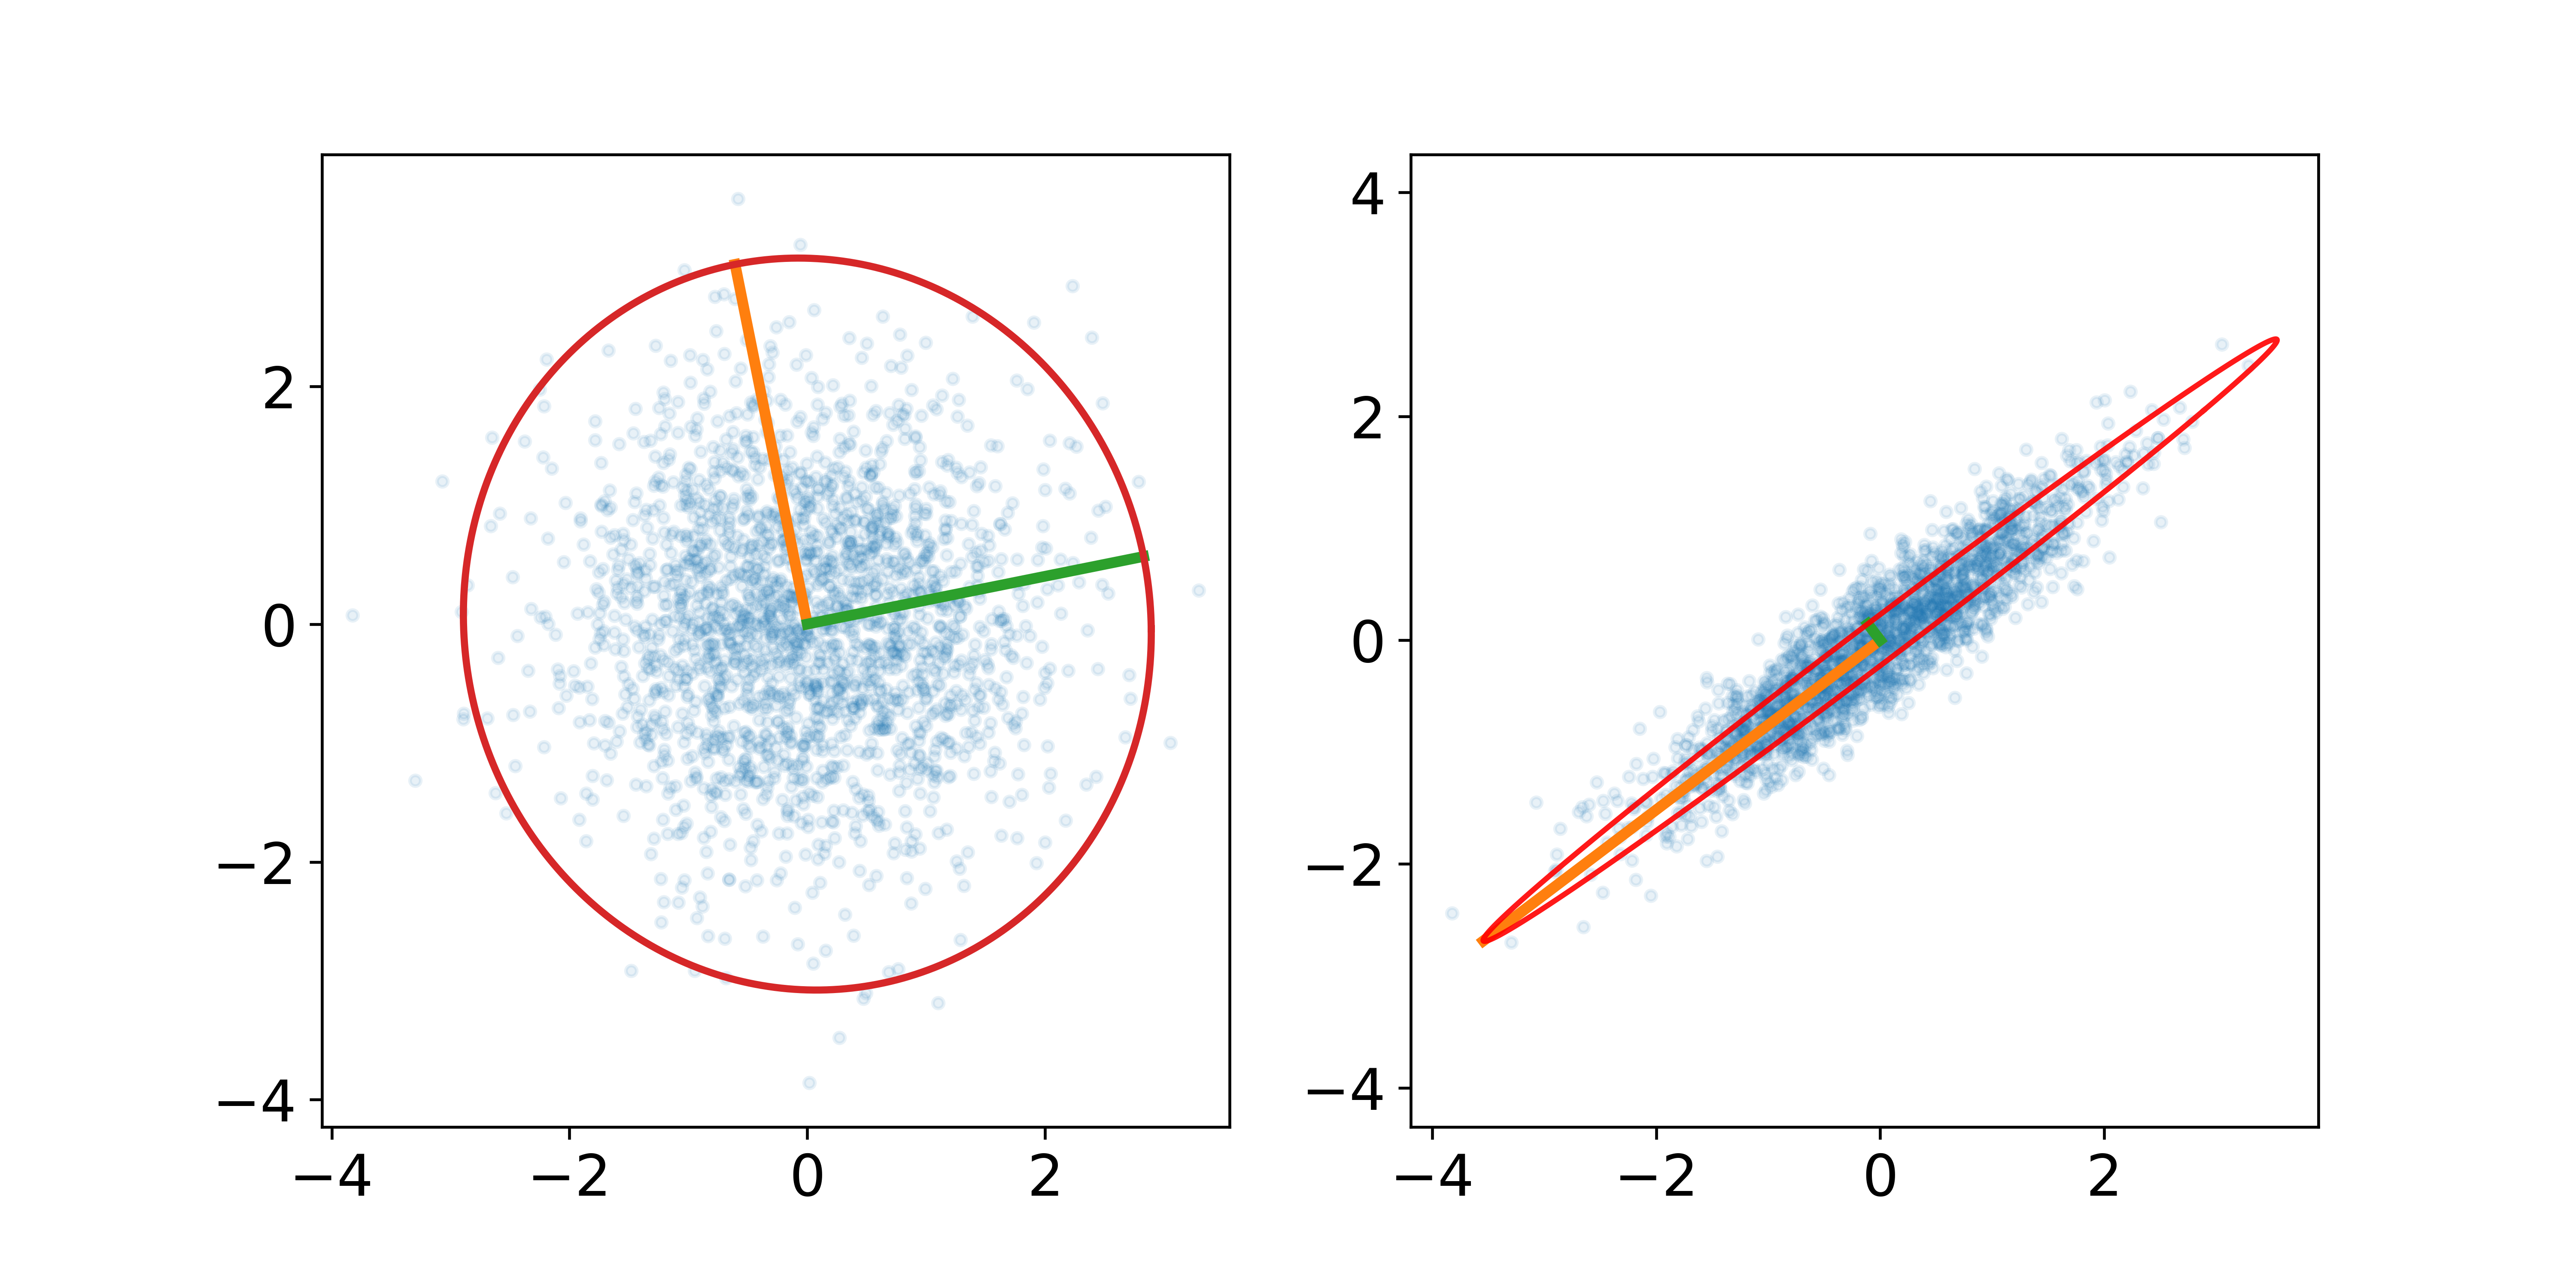
\includegraphics[width = 0.5\textwidth]{pca.png}
% \end{figure}
% \end{frame}

\end{document}
% -*- root: ../assignment.tex -*-
\subsection*{Least Squares}
\begin{enumerate}[resume]
    \item The least square approximate solution to  problem $\mf{Ax} = b, \mf{A} \in \mb{R}^{m \times n}$ is obtained by minimizing the following objective fucntion,
    \[ O\lp\mf{x}\rp = \lV\mf{Ax} - \mf{b}\rV^2 = \sum_{i=1}^{m} \lp\tilde{\mf{a}}_i^T\mf{x} - \mf{b}_i\rp^2 \]
    If the the objective function was defined differently, where the different components were given different weights for the different terms, 
    \[ O_w\lp\mf{x}\rp = \sum_{i=1}^{m} w_i\lp\tilde{\mf{a}}_i^T\mf{x} - \mf{b}_i\rp^2 \]
    This is the \textit{weighted least squares}. Find the expression for the approximate solution of the weighted least squares problem.

    \item Consider a matrix $\mf{A} \in \mb{R}^{m \times n}$ with independent columns. There is no matrix $\mf{X}$, such that $\mf{A}\mf{X} = \mf{I}$. Find an expression for the matrix $\mf{X}$, such that $\lV\mf{A}\mf{X} - \mf{I}\rV^2$ is minimum. Hint: Consider the individual columns of $\mf{X}$ and $\mf{I}$.

    \item Consider the following polynomial equation,
    \[ y = \sum_{i=0}^{n} \beta_ix^i, \,\,\,\, x, y, \beta_i \in \mb{R} \]
    This expression is linear in the polynomial coefficients. Fitting a polynomial to data can be done through a linear least square procedure. Conisder a set of measurements $\lc\lp x_l, y_l \rp\rc_{l=1}^{m}$. We are interested in fitting a polynomial that fits this data, such that the difference between the polynomial and data is as low as possible.
    \[ \bmxc y_1\\ y_2\\ \vdots \\ y_m\emxc = \bmxc 1 & x_1 & x_1^2 & \ldots & x_1^n\\ 1 & x_2 & x_2^2 & \ldots & x_2^n\\ \vdots & \vdots & \vdots & \ddots & \vdots\\ 1 & x_m & x_m^2 & \ldots & x_m^n \emxc \bmxc\beta_0 \\ \beta_1 \\ \beta_2 \\ \vdots \\ \beta_n\emxc \]
    \[ \mf{y} = \mf{X}\mf{\beta} \]

    $\mf{X}$ is called the \textit{Vandermonde} matrix. To estimate $\beta$ through a least squares procedure, $\mf{X}$ must have independent columns. Prove that for a set of different $x_i$s the \textit{Vandermonde} matrix has independent columns.

    You are provided with CSV format data file (polyfit.csv) containing data $\lc\lp x_l, y_l \rp\rc_{l=1}^{m}$, to which you are required to fit a polynomial function. The choice of the order of the polynomial is up to you. This can be come from \textit{a priori} knowledge of the system from which data is collected, or it can be decided based on eyeballing the scatter plot between $x_i$ and $y_i$. 

    \begin{enumerate}
        \item \textbf{Data fitting error}: Fit polynomials of orders 0 to 10 to the given data, and for each order determine the data fitting error.
        \[ e_n = \lV\mf{X}\hat{\beta} - \mf{y}\rV \]
        Plot $e_n$ versus the polynomial model order $n$. You should observe the fitting error to monotonically decrease as a function fo $n$. Why is this? Can $e_n$ ever be zero?

        \item \textbf{Model validation}: Even though increasing the polynomial order decreases the data fitting error, this is not always desirable. Given that noise in ubiquitous in all measurements, increasing model order will result in a polynomial that not only fits the general trend in the data, but also the observed measurement noise. Thus, the optimal choice for the model order is determined through a validation procedure, where the data is split into two sets - \textit{training} set and a \textit{testing} set. In order to understand this, you are required to:
        \begin{enumerate}
            \item Split your data $D$ into two sets of size 80\% and 20\%, corresponding to the \textit{training} $D_{train}$ and \textit{testing} $D_{test}$ sets; these percentages are arbitrary. Split you data randomly, such that each data entry is randomly assigned to $D_{train}$ and $D_{test}$.

            \item Fit the polynomial model of a particular order to $D_{train}$. Let the model parameters obtained be $\hat{\beta}$. The validation error for this model is defined as the following.
            \[ e_n^{val} = \lV\mf{X}\hat{\beta} - \mf{y}\rV \]
            where, $\mf{X}$ and $\mf{y}$ comes from the test data set $D_{test}$. Estimate the validation error for different models order 0 to 10, and plot $e_n^{val}$ versus the polynomial model order $n$. How is this plot different from the plot $e_n$ versus $n$? What is the optimal choice for the model order based on the validation procedure?
        \end{enumerate}

        \item \textbf{Regularized data fitting}: Instead of minimzing $\lV\mf{X}\beta - \mf{y}\rV^2$ of the data, now fit a model that minimizes, $\lV\mf{X}\beta - \mf{y}\rV^2 + \lambda\beta^T\beta$, where $\lambda \geq 0$. In this particular case fit the model order to a high value (e.g. 10) and the entire data set $D$. Perform the data ditting procedure for different values of $\lambda$. Plot $\lV\mf{X}\beta - \mf{y}\rV$ verus $\lambda$. Compare the values of $\hat{\beta}$ for the different values of $\lambda$ and compare these to your optimal choice of model parameters from the previous question.
    \end{enumerate}

    \item Consider a time series $\mf{x} = \lc x_0, x_1,\ldots x_{N-1} \rc$ consisting of $N$ data points, where $n$ indicates time index. The time series is corrupted by noise, and we are interested in filtering the time series to obtain a smooth estimate of the the general trend in the time series. This can be posed a problem of estimating a new time series $\hat{\mf{x}}$, such that the difference $\mf{x} - \hat{\mf{x}}$ is minimized and $\hat{\mf{x}}$ is smooth, i.e. the adjacent values of the signal do not change abruptly. 
    \[ O\lp \hat{x} \rp = \sum_{i = 1}^{N} \lp x_i - \hat{x}_i \rp^2 + \lambda \sum_{i = 2}^{N-1} \lp 2 \hat{x}_i - \hat{x}_{i-1} - \hat{x}_{i+1} \rp^2 \]

    If $\mf{x}$ and $\hat{\mf{x}}$ are considered as $N$-vectors, then this can eb written as 
    \[ O\lp \hat{\mf{x}} \rp = \lV \mf{x} - \hat{\mf{x}} \rV^2 + \lambda \lV \mf{D}\hat{\mf{x}} \rV^2 \]

    You are provided with a CSV data file (timeseries.csv) consisting of a time series. Filter this time series by minimizing $O\lp\hat{\mf{x}}\rp$ for different values of $\lambda$. Plot $\mf{x}$ and $\hat{\mf{x}}$ for different values of $\lambda$. What role does $\lambda$ play in the minimzation problem?

    \item Consider the following resistive network, where the horizontal resistors have resistnce of $R_h = 1\Omega$ and the vertical resistors have a resistance of $R_v = 2\Omega$. You goal is to determine a set of currents in the $\mf{i} = \bmx i_1 & i_2 & \ldots & i_{16}\emx^T$, so as to acheive a particular distribution of potentials at the different nodes of the network. Node that we have control only over the currents at the edge nodes, and in the internal nodes the current is zero, i.e. $i_6 = i_7 = i_{10} = i_{11} = 0$.

    \begin{center}
    \begin{circuitikz}[scale=0.8, transform shape]
        \draw (0,0) to[R,*-*] (0,2) to[R,*-*] (0,4) to[R,*-*] (0,6);
        \draw (2,0) to[R,*-*] (2,2) to[R,*-*] (2,4) to[R,*-*] (2,6);
        \draw (4,0) to[R,*-*] (4,2) to[R,*-*] (4,4) to[R,*-*] (4,6);
        \draw (6,0) to[R,*-*] (6,2) to[R,*-*] (6,4) to[R,*-*] (6,6);

        \draw (0,0) to[R,*-*] (2,0) to[R,*-*] (4,0) to[R,*-*] (6,0);
        \draw (0,2) to[R,*-*] (2,2) to[R,*-*] (4,2) to[R,*-*] (6,2);
        \draw (0,4) to[R,*-*] (2,4) to[R,*-*] (4,4) to[R,*-*] (6,4);
        \draw (0,6) to[R,*-*] (2,6) to[R,*-*] (4,6) to[R,*-*] (6,6);

        \draw (-1,7) node[above]{{\Large $i_1$}} to[short, o-] (0,6);
        \draw (2,7) node[above]{{\Large $i_2$}} to[short, o-] (2,6);
        \draw (4,7) node[above]{{\Large $i_3$}} to[short, o-] (4,6);
        \draw (7,7) node[above]{{\Large $i_4$}} to[short, o-] (6,6);

        \draw (7,2) node[right]{{\Large $i_{12}$}} to[short, o-] (6,2);
        \draw (7,4) node[right]{{\Large $i_{5}$}} to[short, o-] (6,4);

        \draw (-1,-1) node[below]{{\Large $i_{16}$}} to[short, o-] (0,0);
        \draw (2,-1) node[below]{{\Large $i_{15}$}} to[short, o-] (2,0);
        \draw (4,-1) node[below]{{\Large $i_{14}$}} to[short, o-] (4,0);
        \draw (7,-1) node[below]{{\Large $i_{13}$}} to[short, o-] (6,0);

        \draw (-1,2) node[left]{{\Large $i_{9}$}} to[short, o-] (0,2);
        \draw (-1,4) node[left]{{\Large $i_{8}$}} to[short, o-] (0,4);

        \draw (0,6) node[below right]{{\large $v_1$}};
        \draw (2,6) node[below right]{{\large $v_2$}};
        \draw (4,6) node[below right]{{\large $v_3$}};
        \draw (6,6) node[below right]{{\large $v_4$}};

        \draw (0,4) node[below right]{{\large $v_8$}};
        \draw (2,4) node[below right]{{\large $v_7$}};
        \draw (4,4) node[below right]{{\large $v_6$}};
        \draw (6,4) node[below right]{{\large $v_5$}};

        \draw (0,2) node[below right]{{\large $v_9$}};
        \draw (2,2) node[below right]{{\large $v_{10}$}};
        \draw (4,2) node[below right]{{\large $v_{11}$}};
        \draw (6,2) node[below right]{{\large $v_{12}$}};

        \draw (0,0) node[below right]{{\large $v_{16}$}};
        \draw (2,0) node[below right]{{\large $v_{15}$}};
        \draw (4,0) node[below right]{{\large $v_{14}$}};
        \draw (6,0) node[above right]{{\large $v_{13}$}};

        \node at (1, 6.5) {$R_h$};
        \node at (-0.6, 5) {$R_v$};
     \end{circuitikz}
     \end{center}

    Let $\mf{v} = \bmx v_1 & v_2 & \ldots & v_{16}\emx$ represent the vector of potential distributions in the network. Then determine $\mf{i}$ such that $\lV\mf{v}_T - \mf{v}\rV^2$ is minimized for the followingdesired potential distribution (Note that the potentias are arragned in a matrix $\mf{V}_{map} = \bmxc 
    v_{1} & v_{2} & v_{3} & v_{4}\\
    v_{8} & v_{7} & v_{6} & v_{5}\\
    v_{9} & v_{10} & v_{11} & v_{12}\\
    v_{16} & v_{15} & v_{14} & v_{13}
    \emxc$
    \begin{enumerate}
        \item $\mf{V}_{map} = \bmxc 
        1 & 2 & 3 & 4\\
        1 & 2 & 3 & 4\\
        1 & 2 & 3 & 4\\
        1 & 2 & 3 & 4
        \emxc $ 
        \item $\mf{V}_{map} = \bmxc 
        2 & 2 & 2 & 2\\
        2 & 1 & 1 & 2\\
        2 & 1 & 1 & 2\\
        2 & 2 & 2 & 2
        \emxc $
        \item $\mf{V}_{map} = \bmxc 
        1 & 1 & 1 & 1\\
        0 & 0 & 0 & 0\\
        0 & 0 & 0 & 0\\
        1 & 1 & 1 & 1
        \emxc $ 
    \end{enumerate}
    for some desired potential distribution $\mf{v}_T$, subject to the constraint $\sum_{k=1}^{16} i_k = 0$.

    \item Trialteration is a process of determining the position $\mf{x} = \bmx x_1 & x_2\emx^T$ of a point $P$ given the distance of the point from a $N$ control points of known locations $\mf{a}_1, \mf{a}_2, \ldots \mf{a}_N$. At any given point in time $n$, we have $N$ different measurements corresponding to the distance of the point $P$ from the $N$ control points, i.e.
    \[ \mf{d}_n = \bmx d_{n1} & d_{n2} & \ldots & d_{nN}\emx^T \]
    where, $d_{ni}^2 = \lV\mf{x}_n - \mf{a}_i\rV_2^2$ for all $1 \leq i \leq N$.
    \begin{center}
    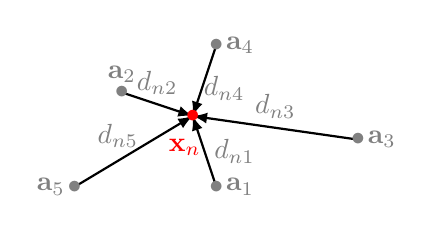
\begin{tikzpicture}[scale=0.6]
        \draw[thick,-latex] (0,0) -- (-0.5, 1.5);
        \node[gray, right] at (-0.25, 0.75) {$d_{n1}$};

        \draw[thick,-latex] (-2,2) -- (-0.5, 1.5);
        \node[gray, above] at (-1.25, 1.75) {$d_{n2}$};

        \draw[thick,-latex] (3,1) -- (-0.5, 1.5);
        \node[gray, above] at (1.25, 1.25) {$d_{n3}$};

        \draw[thick,-latex] (0,3) -- (-0.5, 1.5);
        \node[gray, xshift=0.25cm, yshift=0.2cm] at (-0.25, 1.75) {$d_{n4}$};

        \draw[thick,-latex] (-3,0) -- (-0.5, 1.5);
        \node[gray, xshift=-0.2cm, yshift=0.2cm] at (-1.75, 0.75) {$d_{n5}$};

        \node[gray] at (0,0) {$\bullet$};
        \node[gray, right] at (0,0) {$\mf{a}_1$};
        \node[gray] at (-2,2) {$\bullet$};
        \node[gray, above] at (-2,2) {$\mf{a}_2$};
        \node[gray] at (3,1) {$\bullet$};
        \node[gray, right] at (3,1) {$\mf{a}_3$};
        \node[gray] at (0,3) {$\bullet$};
        \node[gray, right] at (0,3) {$\mf{a}_4$};
        \node[gray] at (-3,0) {$\bullet$};
        \node[gray, left] at (-3,0) {$\mf{a}_5$};
        \node[red] at (-0.5,1.5) {$\bullet$};
        \node[red, xshift=-0.1cm, yshift=-0.1cm] at (-0.5,1) {$\mf{x}_n$};
    \end{tikzpicture}
    \end{center}

    $\mf{x}_n$ are nonlinear functions of the measurements and the control point locations. However, taking the difference between two squared distance measurements $d_j^2$ and $d_i^2$ results in linear equations in the unknown coordinates,
    \[ \lp \mf{a}_i - \mf{a}_j\rp^T\mf{x} = \frac{\lp d_j^2 - \lV\mf{a}_j\rV_2^2 \rp - \lp d_i^2  - \lV\mf{a}_i\rV_2^2 \rp}{2} \]

    Consider the point $P$ that moves with time; $\mf{x}_n \in \mb{R}^{2}$ represents the location of the point at time instant $n$. The distance of this point from a set of 50 different control points is given to you in a CSV data file (trilatdist.csv); the data rows correspond to distance measurements from the different control points at a given point in time, while the colums correpond to the distance of the point from a particular control point for all time. The locations of the 50 control points are available in a separate fileCSV file (trilatctrlpos.csv). Each of these distance measurements is affected by noise. You aim is to use these distance measurements to reconstruct the trajecotry of the point $\mf{x}_n$ as a function of time.
    \begin{enumerate}
        \item What is the minimum number of distance measurements you need to estimate the unknown coordinates of the point $\mf{x}$?
        \item You are provided the actual trajectory of point $P$ in the file trilatactpos.csv. How does you estimate compare with that of the actual trajectory? If we are informed that the point $P$ does not undergo large changes in position between two consecutive time instants $n-1$ and $n$, how would you use this information to improve your estimate?
    \end{enumerate}
\end{enumerate}
% \vfill
% % -*- root: ../assignment.tex -*-
\subsection*{Linear Dynamics Systems -- Transfer function view}
\begin{enumerate}[resume]
    \item Write down the differential equation representing relationship between the loop current $y\ct{t}$ and the input voltage $v\ct{t}$. Assume a initial loop current of $y\ct{0^-} = y_0$.
    \begin{center}
        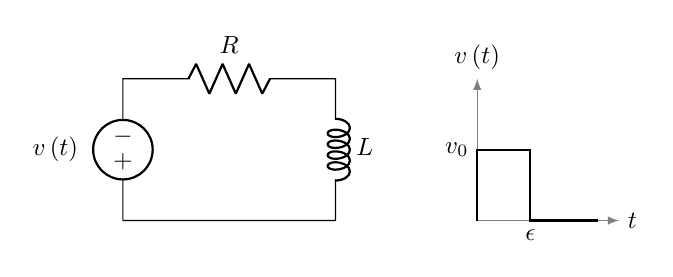
\begin{tikzpicture}[scale=0.9, transform shape]
        \path (0,0) coordinate (ref_gnd);
        \draw
          (ref_gnd) to[american voltage source=$v\lp t\rp$] ++(0,2)
                    to[R=\(R\)] ++(3,0) 
                    to[L=\(L\)] ++(0,-2) 
          -- (ref_gnd);
        
        \draw[-latex, gray] (5, 0) -- (7, 0) node[black, right] {$t$};
        \draw[-latex, gray] (5, 0) -- (5, 2) node[black, above] {$v\ct{t}$};
        \draw[-, black, thick] (5, 0) -- (5, 1) -- (5.75, 1) -- (5.75, 0) -- (6.7, 0);
        \node[black, left] at (5, 1) {$v_0$};
        \node[black, below] at (5.75, 0) {$\epsilon$};
        \end{tikzpicture}
    \end{center}
    \begin{enumerate}
        \item Find the response of the system for the input $v\ct{\bullet}, \forall t \geq 0$ shown in the figure.
        \item Show that for a suitable choice $\epsilon$, $y\ct{t} = 0, \,\, \forall t > \epsilon$.
        \item Assuming $y\ct{0^-} = 0$, what happens to $y\ct{t}$ when, $\epsilon \to 0$ and $v_0 \to \frac{1}{\epsilon}$? Derive the mathematical expression applying this limit. Compare this solution to the input $v\ct{t} = \delta\ct{t}$.
        \item What will happen when $\epsilon \to 0$ and $v_0$ is constant?  
    \end{enumerate}

    \item Derive the differential equation governing the following two mechanical systems. The input to both these systems is the force $f\ct{t}$, and the position $x\ct{t}$ is the output; assume the initial conditions to $x\ct{0^-}, \dot{x}\ct{0^-}$.

    \begin{center}
    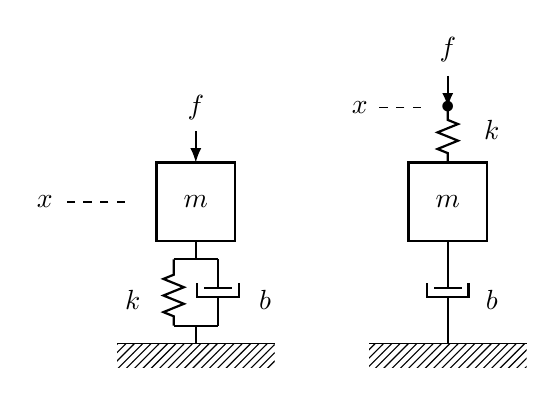
\begin{tikzpicture}[every node/.style={draw,outer sep=0pt,thick}, scale=0.8]
    %define the spring
    \tikzstyle{spring}=[thick,decorate,decoration={zigzag,pre length=0.12cm,post length=0.12cm,amplitude=1.3mm,segment length=6}]

    %define the dashpot
    \tikzstyle{damper}=[thick,decoration={markings,
      mark connection node=dmp,
      mark=at position 0.5 with 
      {
          \node (dmp) [thick,inner sep=0pt,transform shape,rotate=-90,minimum width=15pt,minimum height=3pt,draw=none] {};    
          \draw [thick] ($(dmp.north east)+(2pt,0)$) -- (dmp.south east) -- (dmp.south west) -- ($(dmp.north west)+(2pt,0)$);
          \draw [thick] ($(dmp.north)+(0,-5pt)$) -- ($(dmp.north)+(0,5pt)$);
      }
    }, decorate]

    %define the spring-dashpot
    \tikzstyle{spr-dash}=[thick,decorate,decoration={markings,
      mark connection node=sqr,
      mark=at position 0.5 with
      {
          \node (sqr) [thick,minimum width=16pt,minimum height=24pt,draw=none] {};
          \draw [thick] (sqr.north west) -- (sqr.north east);
          \draw [thick] (sqr.south west) -- (sqr.south east);
          \draw [spring] (sqr.south west) -- (sqr.north west);
          \draw [damper] (sqr.south east) -- (sqr.north east);
      }
      }]

    %define the ground
    \tikzstyle{ground}=[fill,pattern=north east lines,draw=none, minimum width=0.75cm, minimum height=0.3cm]

    %define node stype
    \tikzset{simplenode/.append style={draw=none}}

    \begin{scope}[xshift=0.0cm]
    %draw the frame mass
    \node (M1) [minimum width=1cm,minimum height=1cm] {$m$};
    
    \node (ground-medium) at (M1.south) [ground,yshift=-1.3cm,minimum width=2cm,anchor=north] {};
    \draw (ground-medium.north west) -- (ground-medium.north east);

    \draw [spr-dash] (ground-medium.north) -- (M1.south);
    \node [draw=none] at ($(ground-medium.north)+(-1cm,0.7cm)$) {$k$};
    \node [draw=none] at ($(ground-medium.north)+(1.1cm,0.7cm)$) {$b$};

    \draw [dashed,thin] (M1.west) ++ (-0.5cm, 0) -- +(-1.0cm, 0);
    \node [draw=none, left] at ($(M1.west) + (-1.5cm, 0cm)$) {$x$};

    \draw [-latex,thick] (M1.north) ++ (0, 0.5cm) -- (M1.north);
    \node [draw=none, yshift=0.7cm] at (M1.north) {$f$};
    \end{scope}

    \begin{scope}[xshift=4.0cm]
    %draw the frame mass
    \node (M1) [minimum width=1cm,minimum height=1cm] {$m$};
    \node (ground-medium) at (M1.south) [ground,yshift=-1.3cm,minimum width=2cm,anchor=north] {};
    \draw (ground-medium.north west) -- (ground-medium.north east);

    \draw [damper] (ground-medium.north) -- (M1.south);
    \draw [spring] (M1.north) -- (0, 1.5cm);
    \node [draw=none] at ($(ground-medium.north)+(0.7cm,3.4cm)$) {$k$};
    \node [draw=none] at ($(ground-medium.north)+(0.7cm,0.7cm)$) {$b$};

    \draw [dashed,thin] (M1.west) ++ (0.2cm, 1.5) -- +(-0.75cm, 0);
    \node [draw=none, left] at ($(M1.west) + (-0.5cm, 1.5cm)$) {$x$};

    \draw [-latex,thick] (0, 2.0cm) -- (0, 1.5cm);
    \node[simplenode] at (0, 1.5cm) {$\bullet$};
    \node [draw=none, yshift=0.1cm] at (0, 2.3) {$f$};
    \end{scope}
    \end{tikzpicture}
    \end{center}

    Find the expression for the step response of these two systems. 

    \item Consider a continuous-time LTI system with impulse response, $h\ct{t} = e^{-2t}1\ct{t}$. What is the output of this system to the following inputs using the convolution integral?
    \begin{enumerate*}
        \item $e^{-2t}1\ct{t}$;
        \item $e^{-2t}$;
        \item $e^{-1t}$;
        \item $e^{-4t}$; and 
        \item $\cos\ct{\omega t}$.
    \end{enumerate*}

    Now, obtain the expression for the output of the system for the above inputs using the system's transfer function $H\ct{s}$.

    \item Find the impulse response and transfer functions of the following composition of subsystems with individual impulse response $h_i\ct{t}$.
    \begin{center}
        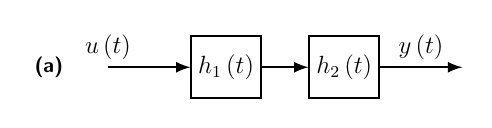
\begin{tikzpicture}[scale=0.75, transform shape, thick, node distance=2cm]
        \draw
            node [input, name=input1] {} 
            node [block, right of=input1] (sys1) {{\large $h_1\ct{t}$}}
            node [block, right of=sys1] (sys2) {{\large $h_2\ct{t}$}}
            node [input, right of=sys2, name=output1] {};
            \draw[-latex] node [above] {{\large $u\ct{t}$}} (input1) -- node {} (sys1);
            \draw[-latex](sys1) -- node {} (sys2);
            \draw[-latex](sys2) -- node[above] {\large $y\ct{t}$} (output1);
            \node[]  at (-1,0) {\textbf{(a)}};
        \end{tikzpicture}

        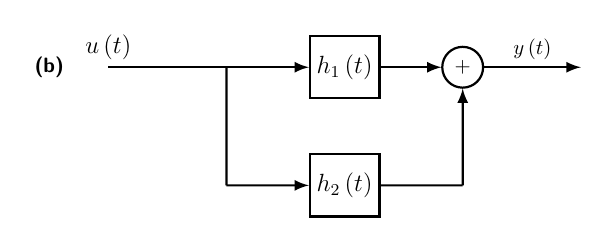
\begin{tikzpicture}[scale=0.75, transform shape, thick, node distance=2cm]
        \draw
            node [input, name=input1] {}
            node [input, right of=input1, name=tempin1] {} 
            node [input, below of=tempin1, name=tempin2] {} 
            node [block, right of=tempin1] (sys1) {{\large $h_1\ct{t}$}}
            node [block, right of=tempin2] (sys2) {{\large $h_2\ct{t}$}}
            node [sum, right of=sys1] (suma1) {$\suma$} 
            node [input, right of=sys2, name=tempout2] {}
            node [input, right of=suma1, name=output1] {};

            \draw[-] node [above] {{\large $u\ct{t}$}} (input1) -- node {} (tempin1);
            \draw[-latex] node {} (tempin1) -- node {} (sys1);
            \draw[-] node {} (tempin1) -- node {} (tempin2);
            \draw[-latex] node {} (tempin2) -- node {} (sys2);
            \draw[-latex](sys1) -- (suma1);
            \draw[-] node {} (sys2) -- node {} (tempout2);
            \draw[-latex] node {} (tempout2) -- node {} (suma1);
            \draw[-latex] node {} (suma1) -- node[above] {$y\ct{t}$} (output1);
            \node[]  at (-1,0) {\textbf{(b)}};
        \end{tikzpicture}

        \begin{tikzpicture}[scale=0.75, transform shape, thick, node distance=2cm]
        \draw
            node [input, name=input1] {}
            node [sum, right of=input1] (suma1) {$\suma$} 
            node [input, below of=suma1, name=tempfb] {} 
            node [block, right of=suma1] (sys1) {{\large $h_1\ct{t}$}}
            node [input, right of=sys1, name=tempout1] {}
            node [input, right of=tempout1, name=output1] {}
            node [input, below of=tempout1, name=tempout2] {}
            node [block, below of=sys1] (sys2) {{\large $h_2\ct{t}$}};

            \draw[-latex] node [above] {{\large $u\ct{t}$}} (input1) -- node {} (suma1);
            \draw[-latex] node {} (suma1) -- node {} (sys1);
            \draw[-] node {} (sys1) -- node {} (tempout1);
            \draw[-latex] node {} (tempout1) -- node {} (output1);
            \draw[-] node {} (tempout1) -- node {} (tempout2);
            \draw[-latex] node {} (tempout2) -- node {} (sys2);
            \draw[-] node {} (sys2) -- node {} (tempin2);
            \draw[-latex] node {} (tempin2) -- node {} (suma1);
            \node[]  at (-1,0) {\textbf{(c)}};
        \end{tikzpicture}
    \end{center}

    \item Consider the second order system, $\ddot{y}\ct{t} + 2\zeta\omega_n\dot{y}\ct{t} + \omega_n^2y\ct{t} = u\ct{t}$. Find the impulse response of this system. Plot the impulse response of the system for $\omega_n = 1$ and the following values of the parameter $\zeta$.
    \begin{enumerate*}
        \item $\zeta = \sqrt{2}$;
        \item $\zeta = 1$;
        \item $\zeta = 0.5$;
        \item $\zeta = 0$;
        \item $\zeta = -0.5$; and 
        \item $\zeta = -1.0$;
    \end{enumerate*}
    For each of these parameter values show the location of the poles of the corresponding transfer function.
\end{enumerate}
% \vfill
% % -*- root: ../assignment.tex -*-
\subsection*{Linear Dynamics Systems -- State space view}
\begin{enumerate}[resume]
    \item Derive the state and measurement equations for the following composite systems, assuming the system $H_i$ to have the parameters $\ct{\mf{A}_i, \mf{B}_i, \mf{C}_i, \mf{D}_i}$.
    \begin{center}
        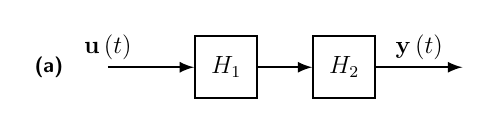
\begin{tikzpicture}[scale=0.75, transform shape, thick, node distance=2cm]
        \draw
            node [input, name=input1] {} 
            node [block, right of=input1] (sys1) {{\large $H_1$}}
            node [block, right of=sys1] (sys2) {{\large $H_2$}}
            node [input, right of=sys2, name=output1] {};
            \draw[-latex] node [above] {{\large $\mf{u}\ct{t}$}} (input1) -- node {} (sys1);
            \draw[-latex](sys1) -- node {} (sys2);
            \draw[-latex](sys2) -- node[above] {\large $\mf{y}\ct{t}$} (output1);
            \node[]  at (-1,0) {\textbf{(a)}};
        \end{tikzpicture}

        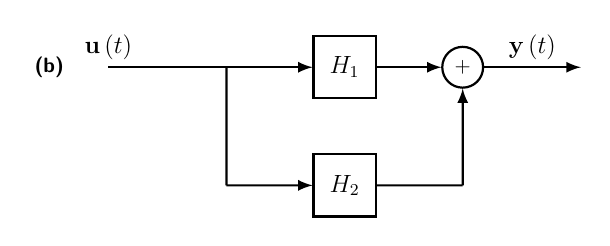
\begin{tikzpicture}[scale=0.75, transform shape, thick, node distance=2cm]
        \draw
            node [input, name=input1] {}
            node [input, right of=input1, name=tempin1] {} 
            node [input, below of=tempin1, name=tempin2] {} 
            node [block, right of=tempin1] (sys1) {{\large $H_1$}}
            node [block, right of=tempin2] (sys2) {{\large $H_2$}}
            node [sum, right of=sys1] (suma1) {$\suma$} 
            node [input, right of=sys2, name=tempout2] {}
            node [input, right of=suma1, name=output1] {};

            \draw[-] node [above] {{\large $\mf{u}\ct{t}$}} (input1) -- node {} (tempin1);
            \draw[-latex] node {} (tempin1) -- node {} (sys1);
            \draw[-] node {} (tempin1) -- node {} (tempin2);
            \draw[-latex] node {} (tempin2) -- node {} (sys2);
            \draw[-latex](sys1) -- (suma1);
            \draw[-] node {} (sys2) -- node {} (tempout2);
            \draw[-latex] node {} (tempout2) -- node {} (suma1);
            \draw[-latex] node {} (suma1) -- node[above] {\large $\mf{y}\ct{t}$} (output1);
            \node[]  at (-1,0) {\textbf{(b)}};
        \end{tikzpicture}

        \begin{tikzpicture}[scale=0.75, transform shape, thick, node distance=2cm]
        \draw
            node [input, name=input1] {}
            node [sum, right of=input1] (suma1) {$\suma$} 
            node [input, below of=suma1, name=tempfb] {} 
            node [block, right of=suma1] (sys1) {{\large $H_1$}}
            node [input, right of=sys1, name=tempout1] {}
            node [input, right of=tempout1, name=output1] {}
            node [input, below of=tempout1, name=tempout2] {}
            node [block, below of=sys1] (sys2) {{\large $H_2$}};

            \draw[-latex] node [above] {{\large $\mf{u}\ct{t}$}} (input1) -- node {} (suma1);
            \draw[-latex] node {} (suma1) -- node {} (sys1);
            \draw[-] node {} (sys1) -- node {} (tempout1);
            \draw[-latex] node {} (tempout1) -- node {} (output1);
            \draw[-] node {} (tempout1) -- node {} (tempout2);
            \draw[-latex] node {} (tempout2) -- node {} (sys2);
            \draw[-] node {} (sys2) -- node {} (tempin2);
            \draw[-latex] node {} (tempin2) -- node {} (suma1);
            \draw[-latex] node {} (tempout1) -- node[above] {\large $\mf{y}\ct{t}$} (output1);
            \node[]  at (-1,0) {\textbf{(c)}};
        \end{tikzpicture}
    \end{center}
    
    \item Derive the state and measurement equation for the following system, where the input is the force $f$ applied to mass $m_2$, and the output is the acceleration of the mass $m_1$ and velocity of mass $m_2$.
    \begin{center}
    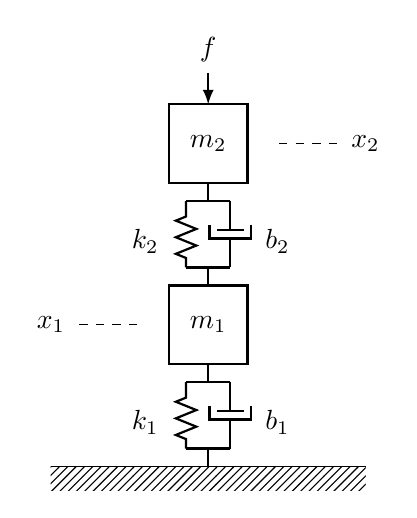
\begin{tikzpicture}[every node/.style={draw,outer sep=0pt,thick}, scale=0.8]
    %define the spring
    \tikzstyle{spring}=[thick,decorate,decoration={zigzag,pre length=0.12cm,post length=0.12cm,amplitude=1.3mm,segment length=6}]

    %define the dashpot
    \tikzstyle{damper}=[thick,decoration={markings,
      mark connection node=dmp,
      mark=at position 0.5 with 
      {
          \node (dmp) [thick,inner sep=0pt,transform shape,rotate=-90,minimum width=15pt,minimum height=3pt,draw=none] {};    
          \draw [thick] ($(dmp.north east)+(2pt,0)$) -- (dmp.south east) -- (dmp.south west) -- ($(dmp.north west)+(2pt,0)$);
          \draw [thick] ($(dmp.north)+(0,-5pt)$) -- ($(dmp.north)+(0,5pt)$);
      }
    }, decorate]

    %define the spring-dashpot
    \tikzstyle{spr-dash}=[thick,decorate,decoration={markings,
      mark connection node=sqr,
      mark=at position 0.5 with
      {
          \node (sqr) [thick,minimum width=16pt,minimum height=24pt,draw=none] {};
          \draw [thick] (sqr.north west) -- (sqr.north east);
          \draw [thick] (sqr.south west) -- (sqr.south east);
          \draw [spring] (sqr.south west) -- (sqr.north west);
          \draw [damper] (sqr.south east) -- (sqr.north east);
      }
      }]

    %define the ground
    \tikzstyle{ground}=[fill,pattern=north east lines,draw=none,minimum width=0.75cm,minimum height=0.3cm]

    \begin{scope}[xshift=5.5cm]
    %draw the frame mass
    \node (M1) [minimum width=1cm,minimum height=1cm] {$m_1$};
     
    %draw the vehicle mass
    \node (M2) at (M1.north) [yshift=+1.8cm, minimum width=1cm, minimum height=1cm] {$m_2$};

    \node (ground-medium) at (M1.south) [ground,yshift=-1.3cm,minimum width=4cm,anchor=north] {};
    \draw (ground-medium.north west) -- (ground-medium.north east);

    \draw [spr-dash] (ground-medium.north) -- (M1.south);
    \node [draw=none] at ($(ground-medium.north)+(-1cm,0.7cm)$) {$k_{1}$};
    \node [draw=none] at ($(ground-medium.north)+(1.1cm,0.7cm)$) {$b_{1}$};
    \draw [spr-dash] (M1.north) -- (M2.south);
    \node [draw=none] at ($(M1.north)+(-1.0cm,0.7cm)$) {$k_{2}$};
    \node [draw=none] at ($(M1.north)+(1.1cm,0.7cm)$) {$b_{2}$};
     
    \draw [-latex,thick] (M2.north) ++ (0, 0.5cm) -- (M2.north);
    \draw [dashed,thin] (M2.east) ++ (0.5cm, 0) -- +(1.0cm, 0);
    \node [draw=none, right] at ($(M2.east) + (1.5cm, 0)$) {$x_{2}$};

    \draw [dashed,thin] (M1.west) ++ (-0.5cm, 0) -- +(-1.0cm, 0);
    \node [draw=none, left] at ($(M1.west) + (-1.5cm, 0cm)$) {$x_{1}$};

    \node [draw=none, yshift=0.7cm] at (M2.north) {$f$};
    \end{scope}
    \end{tikzpicture}
    \end{center}

    Assume now that instead of $f$ the input to this was the position of the mass $m_2$ (i.e. $x_2$) and the output of interest was the acceleration of the mass $m_1$. What would be correspondoing state and measurement equations in this case?

    \item Obtain a state space representation for the following systems:
    \begin{enumerate}
        \item $\sum_{i=0}^n a_iy^{\ct{i}} = \sum_{j=0}^m b_jx^{\ct{j}}$, where $x^{\ct{k}} = \frac{d^k}{dt^k}x\ct{t}$
        \item $\sum_{i=0}^n a_iy\dt{k+i} = \sum_{j=0}^m b_jx\dt{k+j}$
    \end{enumerate}

    \item Write down the state and measurement equations for the following system with the scalar input $u\dt{k}$ and output $\mf{y}\dt{k} = \bmx y_1\dt{k}\\ y_2\dt{k}\emx$. 

    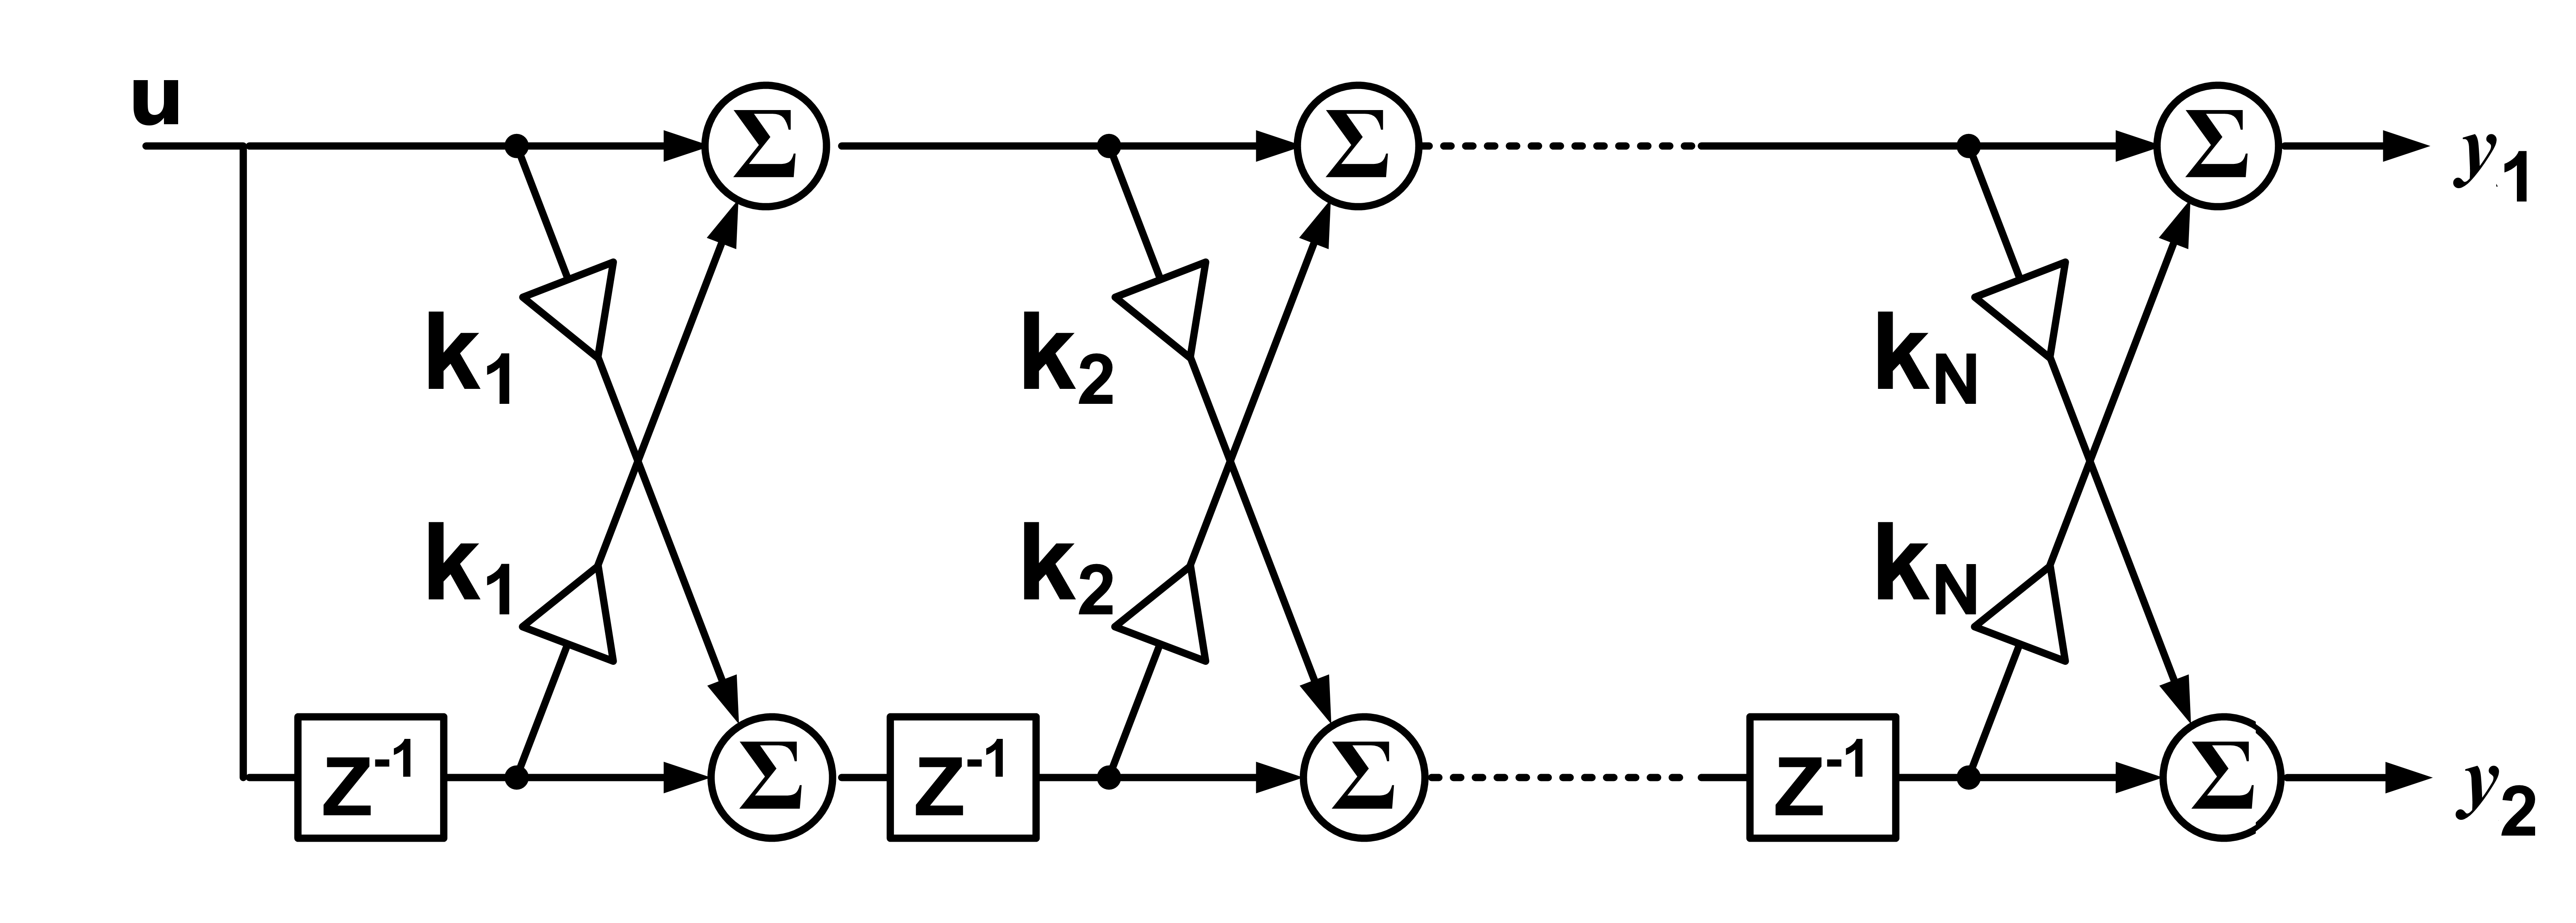
\includegraphics[width=0.45\textwidth]{sections/figs/latticefilt.png}

    \item The following model shows two media and their constituent elements. Medium 1 consists of elements with mass $M_1$ which are interconnected through a spring and damper in parallel with spring constant $k_1$ and damping coefficient $b_1$. Medium 2 consits of elements with mass $M_2$ connected through $k_2$ and $b_2$. At the interface $M_1$ and $M_2$ are connected through $k_3$ nd $b_3$.

    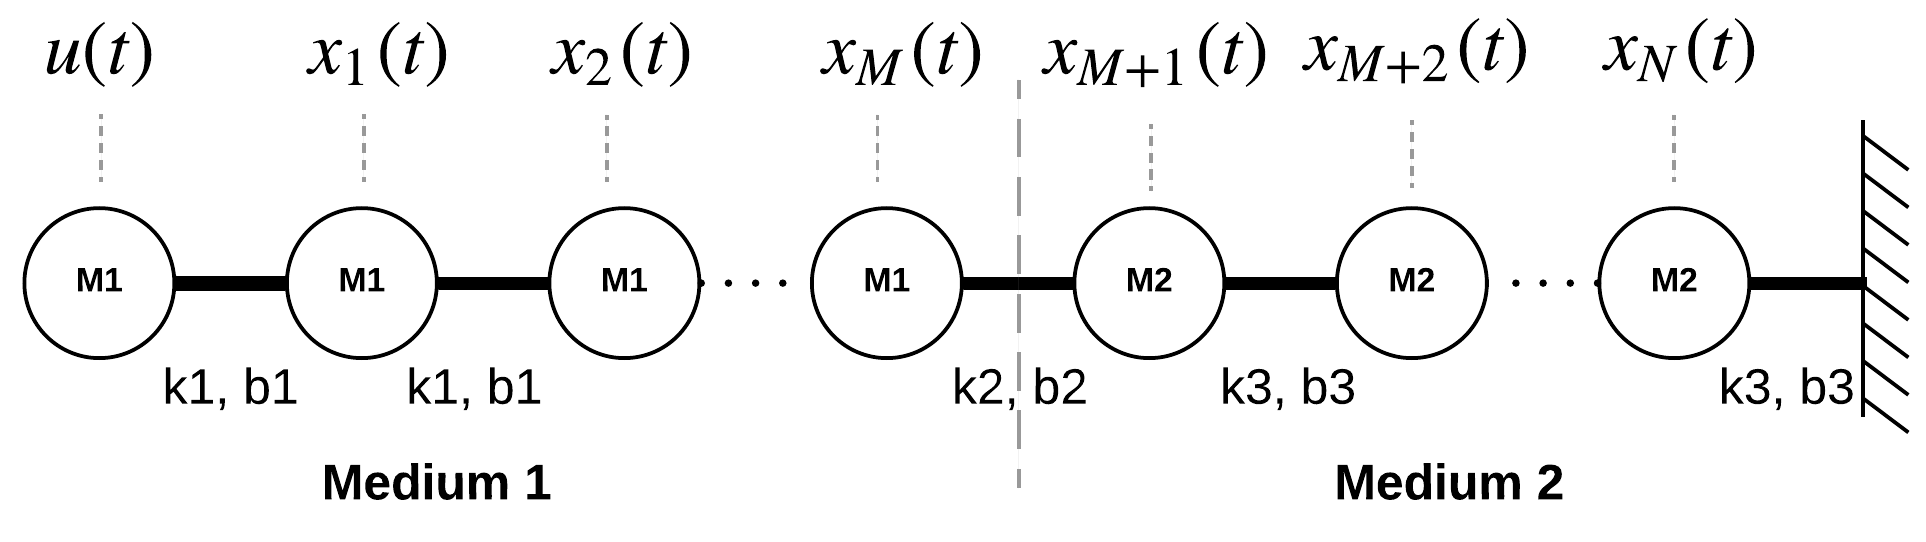
\includegraphics[width=0.45\textwidth]{sections/figs/wavetx.png}    

    The input to this system is $u\ct{t}$ which is the position imposed on the let most element in medium 1. The output of the system are the successive differences in the positions of the massess.
    \[ y_i\ct{t} = x_{i+2}\ct{t} - x_{i+1}\ct{t} \, ,\,\,\, 1 \leq i \leq N-2 \]

    Derive the state and measurement equations for the system.


\end{enumerate}
% \vfill
% % -*- root: ../assignment.tex -*-
% \subsection*{Solution of LDS}
\begin{enumerate}[resume]
    \item Consider $\mf{A} = \bmx 1 & 1 & 0\\ 0 & 0 & 1\\ 0 & 0 & 1\emx$. Compute $\mf{A}^{100}$ and $e^{t\mf{A}}$.

    \item Assuming that $\mf{A} \in \mb{R}^{n \times n}$ is diagonalizable with eigenvalues $\lambda_1, \lambda_2,\ldots \lambda_n$. Prove that the eigenvalues of $e^{\mf{A}}$ are $e^{\lambda_1}, e^{\lambda_2}, \ldots e^{\lambda_n}$

    \item Consider a linear time-variant discrete-time, $\mf{x}\dt{k+1} = \mf{A}\dt{k}\mf{x}\dt{k} + \mf{B}\dt{k}\mf{u}\dt{k}$. Find the general expression for the zero-input solution, and the zero-state solution.

    \item What are the conditions on the individual LTI discrete-time systems $H_1\ct{z}$ and $H_2\ct{z}$ for the following overall system to be:
    \begin{enumerate*}
        \item internally stable;
        \item externally stable;
        \item controllable; and
        \item observable
    \end{enumerate*}
    \begin{center}
        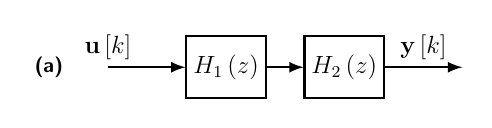
\begin{tikzpicture}[scale=0.75, transform shape, thick, node distance=2cm]
        \draw
            node [input, name=input1] {} 
            node [block, right of=input1] (sys1) {{\large $H_1\ct{z}$}}
            node [block, right of=sys1] (sys2) {{\large $H_2\ct{z}$}}
            node [input, right of=sys2, name=output1] {};
            \draw[-latex] node [above] {{\large $\mf{u}\dt{k}$}} (input1) -- node {} (sys1);
            \draw[-latex](sys1) -- node {} (sys2);
            \draw[-latex](sys2) -- node[above] {\large $\mf{y}\dt{k}$} (output1);
            \node[]  at (-1,0) {\textbf{(a)}};
        \end{tikzpicture}

        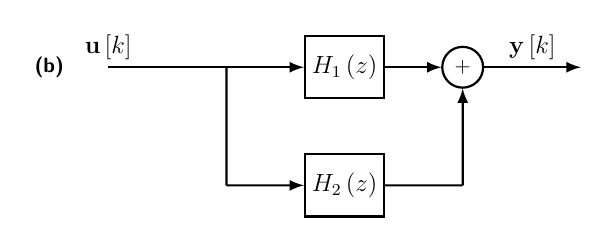
\begin{tikzpicture}[scale=0.75, transform shape, thick, node distance=2cm]
        \draw
            node [input, name=input1] {}
            node [input, right of=input1, name=tempin1] {} 
            node [input, below of=tempin1, name=tempin2] {} 
            node [block, right of=tempin1] (sys1) {{\large $H_1\ct{z}$}}
            node [block, right of=tempin2] (sys2) {{\large $H_2\ct{z}$}}
            node [sum, right of=sys1] (suma1) {$\suma$} 
            node [input, right of=sys2, name=tempout2] {}
            node [input, right of=suma1, name=output1] {};

            \draw[-] node [above] {{\large $\mf{u}\dt{k}$}} (input1) -- node {} (tempin1);
            \draw[-latex] node {} (tempin1) -- node {} (sys1);
            \draw[-] node {} (tempin1) -- node {} (tempin2);
            \draw[-latex] node {} (tempin2) -- node {} (sys2);
            \draw[-latex](sys1) -- (suma1);
            \draw[-] node {} (sys2) -- node {} (tempout2);
            \draw[-latex] node {} (tempout2) -- node {} (suma1);
            \draw[-latex] node {} (suma1) -- node[above] {\large $\mf{y}\dt{k}$} (output1);
            \node[]  at (-1,0) {\textbf{(b)}};
        \end{tikzpicture}

        % \begin{tikzpicture}[scale=0.75, transform shape, thick, node distance=2cm]
        % \draw
        %     node [input, name=input1] {}
        %     node [sum, right of=input1] (suma1) {$\suma$} 
        %     node [input, below of=suma1, name=tempfb] {} 
        %     node [block, right of=suma1] (sys1) {{\large $H_1$}}
        %     node [input, right of=sys1, name=tempout1] {}
        %     node [input, right of=tempout1, name=output1] {}
        %     node [input, below of=tempout1, name=tempout2] {}
        %     node [block, below of=sys1] (sys2) {{\large $H_2$}};

        %     \draw[-latex] node [above] {{\large $\mf{u}\ct{t}$}} (input1) -- node {} (suma1);
        %     \draw[-latex] node {} (suma1) -- node {} (sys1);
        %     \draw[-] node {} (sys1) -- node {} (tempout1);
        %     \draw[-latex] node {} (tempout1) -- node {} (output1);
        %     \draw[-] node {} (tempout1) -- node {} (tempout2);
        %     \draw[-latex] node {} (tempout2) -- node {} (sys2);
        %     \draw[-] node {} (sys2) -- node {} (tempin2);
        %     \draw[-latex] node {} (tempin2) -- node {} (suma1);
        %     \draw[-latex] node {} (tempout1) -- node[above] {\large $\mf{y}\ct{t}$} (output1);
        %     \node[]  at (-1,0) {\textbf{(c)}};
        % \end{tikzpicture}
    \end{center}

    \item Consider a the LTI system, $\dot{\mf{x}}\ct{t} = \mf{A}\mf{x}\ct{t}$, where $\mf{A} \in \mb{R}^{n \times n}$. An experiment was carried out with this system, where the system was started at different initial conditions $\mf{x}_i\ct{0^-}$, and the corresponding state trajectories were recorded to be $\mf{x}_i\ct{t}, \,\, \forall t \geq 0$. Assuming that the set of initial conditions$\lc \mf{x}\ct{0^-} \rc_{i=1}^n$ are linearly independent, find the expression for the $e^{t\mf{A}}$.

    \item Consider the following system, where the input is the force $f$ applied to mass $m_2$, and the output of the system, positions of masses $m_1$ and $m_2$, are measured using a set of position sensors. 
    \begin{enumerate}
        \item Is this system controllable? Is the system still controllable if the input $f$ was acting on the mass $m_1$ instead of $m_2$?
        \item Is this system observable? If instead of measuring both position $x_1$ and $x_2$, if the output of the system was either $x_1$ or $x_2$, is the system still observable?
    \end{enumerate}
    \begin{center}
    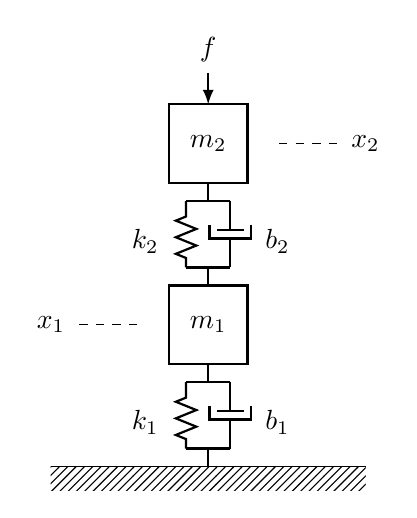
\begin{tikzpicture}[every node/.style={draw,outer sep=0pt,thick}, scale=0.8]
    %define the spring
    \tikzstyle{spring}=[thick,decorate,decoration={zigzag,pre length=0.12cm,post length=0.12cm,amplitude=1.3mm,segment length=6}]

    %define the dashpot
    \tikzstyle{damper}=[thick,decoration={markings,
      mark connection node=dmp,
      mark=at position 0.5 with 
      {
          \node (dmp) [thick,inner sep=0pt,transform shape,rotate=-90,minimum width=15pt,minimum height=3pt,draw=none] {};    
          \draw [thick] ($(dmp.north east)+(2pt,0)$) -- (dmp.south east) -- (dmp.south west) -- ($(dmp.north west)+(2pt,0)$);
          \draw [thick] ($(dmp.north)+(0,-5pt)$) -- ($(dmp.north)+(0,5pt)$);
      }
    }, decorate]

    %define the spring-dashpot
    \tikzstyle{spr-dash}=[thick,decorate,decoration={markings,
      mark connection node=sqr,
      mark=at position 0.5 with
      {
          \node (sqr) [thick,minimum width=16pt,minimum height=24pt,draw=none] {};
          \draw [thick] (sqr.north west) -- (sqr.north east);
          \draw [thick] (sqr.south west) -- (sqr.south east);
          \draw [spring] (sqr.south west) -- (sqr.north west);
          \draw [damper] (sqr.south east) -- (sqr.north east);
      }
      }]

    %define the ground
    \tikzstyle{ground}=[fill,pattern=north east lines,draw=none,minimum width=0.75cm,minimum height=0.3cm]

    \begin{scope}[xshift=5.5cm]
    %draw the frame mass
    \node (M1) [minimum width=1cm,minimum height=1cm] {$m_1$};
     
    %draw the vehicle mass
    \node (M2) at (M1.north) [yshift=+1.8cm, minimum width=1cm, minimum height=1cm] {$m_2$};

    \node (ground-medium) at (M1.south) [ground,yshift=-1.3cm,minimum width=4cm,anchor=north] {};
    \draw (ground-medium.north west) -- (ground-medium.north east);

    \draw [spr-dash] (ground-medium.north) -- (M1.south);
    \node [draw=none] at ($(ground-medium.north)+(-1cm,0.7cm)$) {$k_{1}$};
    \node [draw=none] at ($(ground-medium.north)+(1.1cm,0.7cm)$) {$b_{1}$};
    \draw [spr-dash] (M1.north) -- (M2.south);
    \node [draw=none] at ($(M1.north)+(-1.0cm,0.7cm)$) {$k_{2}$};
    \node [draw=none] at ($(M1.north)+(1.1cm,0.7cm)$) {$b_{2}$};
     
    \draw [-latex,thick] (M2.north) ++ (0, 0.5cm) -- (M2.north);
    \draw [dashed,thin] (M2.east) ++ (0.5cm, 0) -- +(1.0cm, 0);
    \node [draw=none, right] at ($(M2.east) + (1.5cm, 0)$) {$x_{2}$};

    \draw [dashed,thin] (M1.west) ++ (-0.5cm, 0) -- +(-1.0cm, 0);
    \node [draw=none, left] at ($(M1.west) + (-1.5cm, 0cm)$) {$x_{1}$};

    \node [draw=none, yshift=0.7cm] at (M2.north) {$f$};
    \end{scope}
    \end{tikzpicture}
    \end{center}

    % Assume now that instead of $f$ the input to this was the position of the mass $m_2$ (i.e. $x_2$) and the output of interest was the acceleration of the mass $m_1$. What would be correspondoing state and measurement equations in this case?

    % \item Obtain a state space representation for the following systems:
    % \begin{enumerate}
    %     \item $\sum_{i=0}^n a_iy^{\ct{i}} = \sum_{j=0}^m b_jx^{\ct{j}}$, where $x^{\ct{k}} = \frac{d^k}{dt^k}x\ct{t}$
    %     \item $\sum_{i=0}^n a_iy\dt{k+i} = \sum_{j=0}^m b_jx\dt{k+j}$
    % \end{enumerate}

    % \item Write down the state and measurement equations for the following system with the scalar input $u\dt{k}$ and output $\mf{y}\dt{k} = \bmx y_1\dt{k}\\ y_2\dt{k}\emx$. 

    % 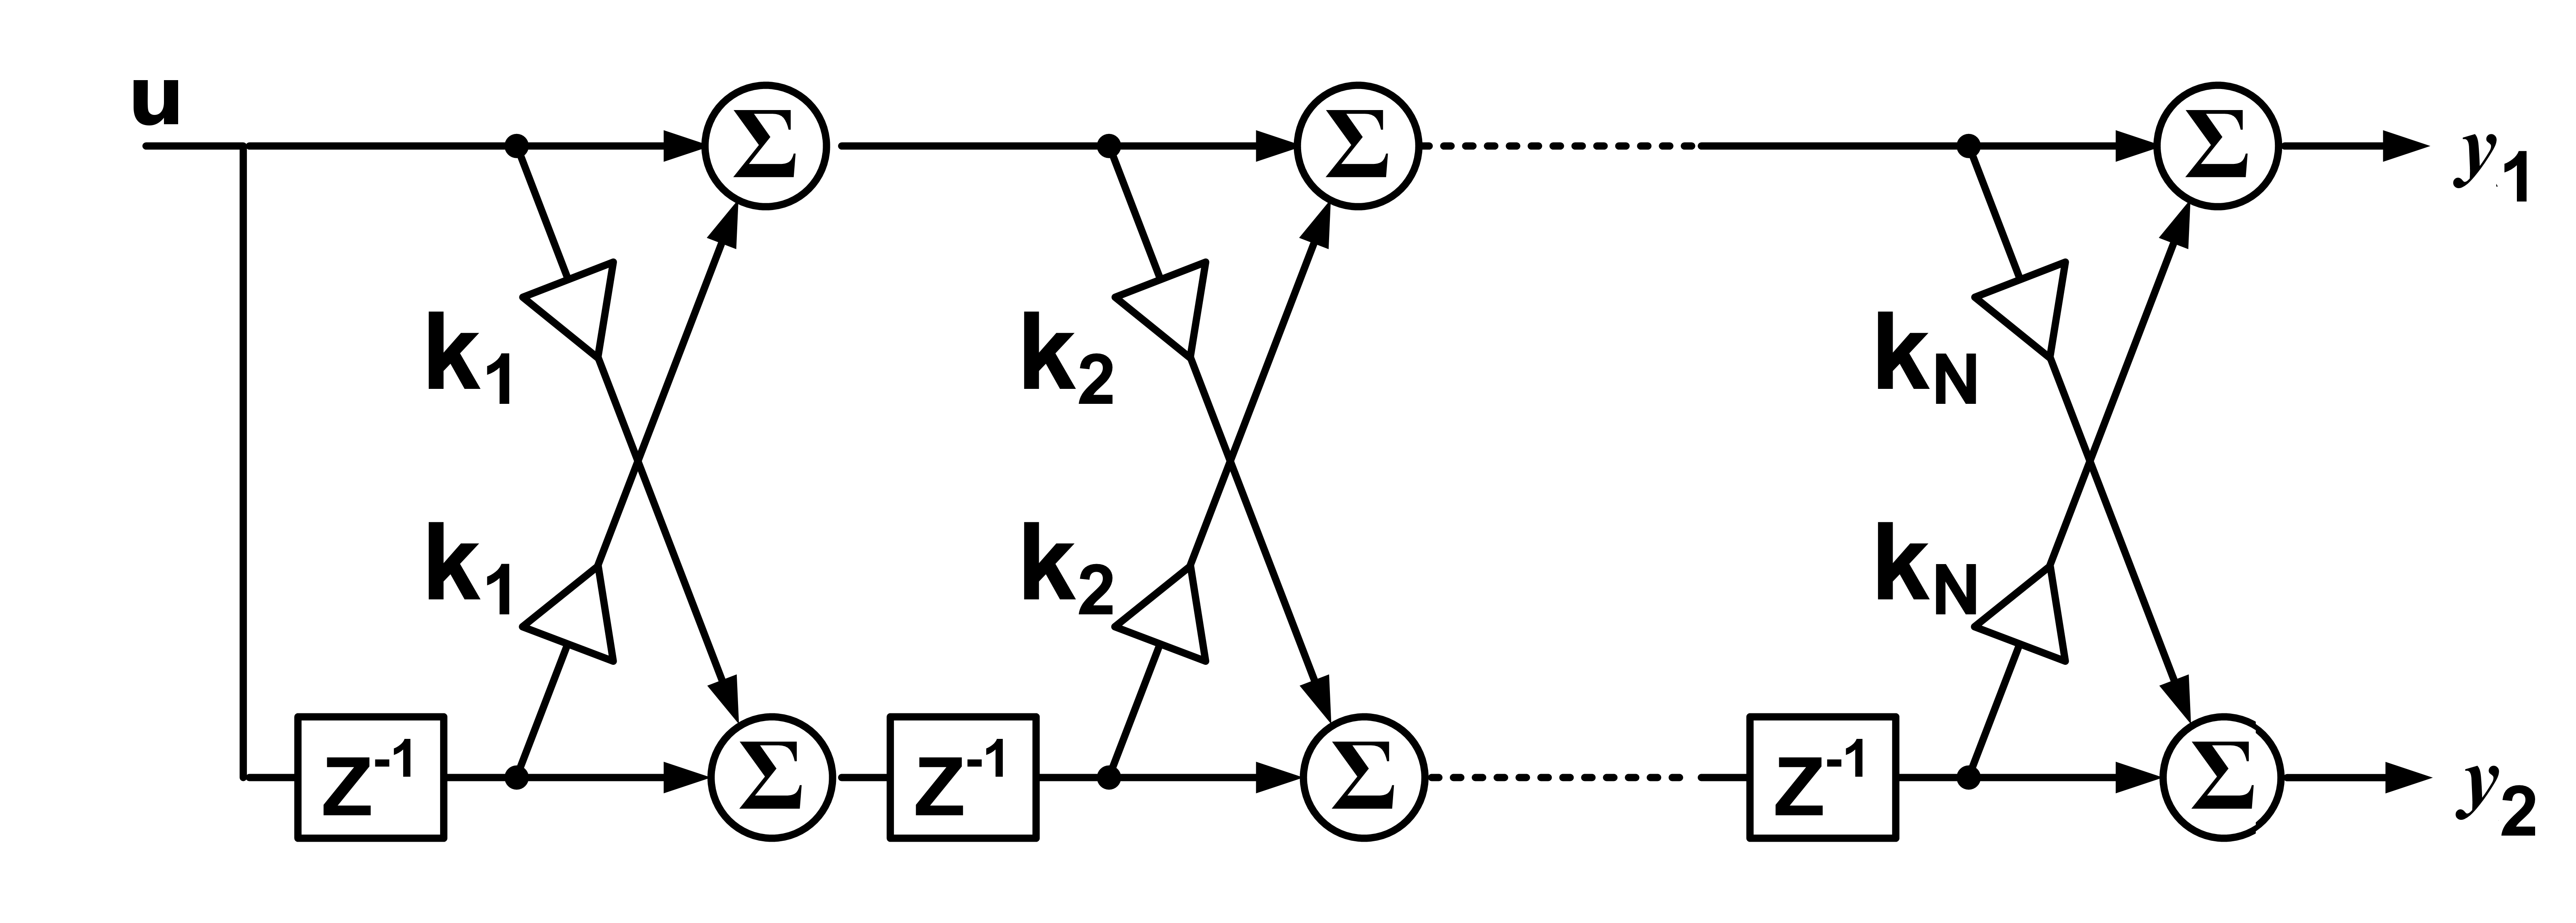
\includegraphics[width=0.45\textwidth]{sections/figs/latticefilt.png}

    % \item The following model shows two media and their constituent elements. Medium 1 consists of elements with mass $M_1$ which are interconnected through a spring and damper in parallel with spring constant $k_1$ and damping coefficient $b_1$. Medium 2 consits of elements with mass $M_2$ connected through $k_2$ and $b_2$. At the interface $M_1$ and $M_2$ are connected through $k_3$ nd $b_3$.

    % 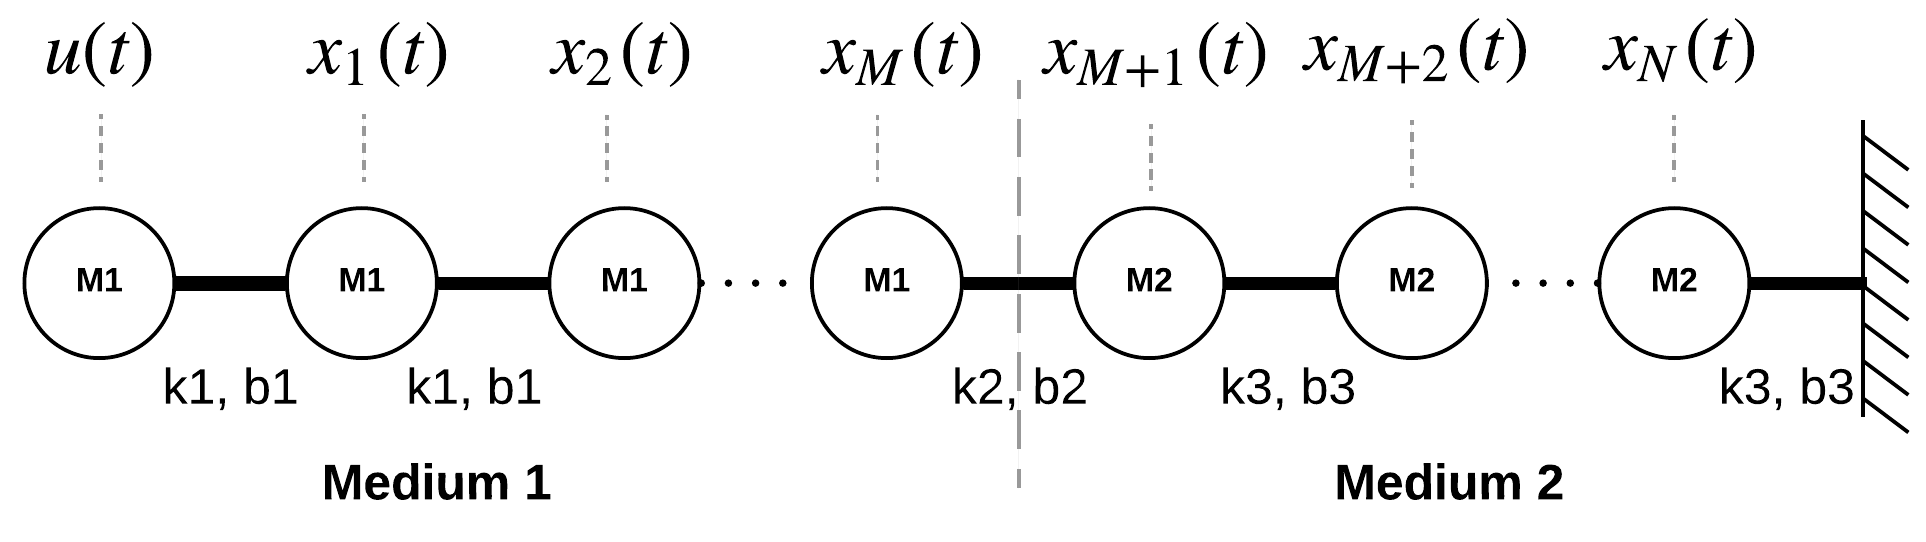
\includegraphics[width=0.45\textwidth]{sections/figs/wavetx.png}    

    % The input to this system is $u\ct{t}$ which is the position imposed on the let most element in medium 1. The output of the system are the successive differences in the positions of the massess.
    % \[ y_i\ct{t} = x_{i+2}\ct{t} - x_{i+1}\ct{t} \, ,\,\,\, 1 \leq i \leq N-2 \]

    % Derive the state and measurement equations for the system.


\end{enumerate}
% \vfill

\newpage
\begin{thebibliography}{50}
\bibitem{strang} G. Strang \textsl{Introduction to linear algebra}.
Wellesley-Cambridge Press Wellesley, MA, USA, 1993
\end{thebibliography}

\end{multicols}
\end{document}